%%%%%%%%%%%%%%%%%%%%%%%%%%%%%%%%%%%%%%%%%
%  My documentation report
%  Objetive: Explain what I did and how, so someone can continue with the investigation
%
% Important note:
% Chapter heading images should have a 2:1 width:height ratio,
% Note, chapter headings were sized incorrectly. Structure.tex has been edited
% accordingly.
% e.g. 920px width and 460px height.
%
%%%%%%%%%%%%%%%%%%%%%%%%%%%%%%%%%%%%%%%%%

%----------------------------------------------------------------------------------------
%	PACKAGES AND OTHER DOCUMENT CONFIGURATIONS
%----------------------------------------------------------------------------------------

\documentclass[11pt]{book} % Default font size

\usepackage[paperwidth=6in,paperheight=9in,top=.5in,bottom=.5in,outer=.75in,inner=.5in,headsep=10pt]{geometry} % Page margins

\usepackage{graphicx}

\usepackage{amssymb}

\usepackage{amsmath}

\usepackage[]{nomencl}

\usepackage{float} 

\usepackage{enumitem}

\usepackage{lipsum}

\usepackage{listings}

\usepackage{wrapfig}

\lstset{
    language=R,
    basicstyle=\footnotesize\ttfamily,
    numbers=left,
    numberstyle=\tiny\color{gray},
    stepnumber=1,
    numbersep=5pt,
    backgroundcolor=\color{white},
    showspaces=false,
    showstringspaces=false,
    showtabs=false,
    frame=tb,
    rulecolor=\color{black},
    tabsize=2,
    captionpos=b,
    breaklines=true,
    breakatwhitespace=false,
    title=\lstname,
    keywordstyle=\color{blue},
    commentstyle=\color{dkgreen},
    stringstyle=\color{mauve},
    escapeinside={\%*}{*)},
    morekeywords={*,...},
    deletekeywords = {data}
}
\usepackage{setspace}

\usepackage{xcolor} % Required for specifying colors by name
\definecolor{ocre}{RGB}{52,177,201} % Define the orange color used for highlighting throughout the book
\definecolor{dkgreen}{rgb}{0, 0.6, 0}
\definecolor{gray}{rgb}{0.5, 0.5, 0.5}
\definecolor{mauve}{rgb}{0.58, 0, 0.82}

% Font Settings
\usepackage{avant} % Use the Avantgarde font for headings
\renewcommand{\familydefault}{\sfdefault}

\usepackage{microtype} % Slightly tweak font spacing for aesthetics
%\usepackage[utf8]{inputenc} % Required for including letters with accents
\usepackage[T1]{fontenc} % Use 8-bit encoding that has 256 glyphs

\usepackage{csquotes}

% Bibliography
\usepackage[style=numeric,sorting=nyt,sortcites=true,autopunct=true,autolang=hyphen,hyperref=true,abbreviate=false,backref=true,backend=bibtex]{biblatex}
\addbibresource{bibliography.bib} % BibTeX bibliography file
\defbibheading{bibempty}{}

%----------------------------------------------------------------------------------------
%	VARIOUS REQUIRED PACKAGES
%----------------------------------------------------------------------------------------

\usepackage{titlesec} % Allows customization of titles

\usepackage{graphicx} % Required for including pictures
\graphicspath{{Pictures/}} % Specifies the directory where pictures are stored

\usepackage{lipsum} % Inserts dummy text

\usepackage{tikz} % Required for drawing custom shapes

\usepackage[english]{babel} % English language/hyphenation

\usepackage{enumitem} % Customize lists
\setlist{nolistsep} % Reduce spacing between bullet points and numbered lists

\usepackage{booktabs} % Required for nicer horizontal rules in tables

\usepackage{eso-pic} % Required for specifying an image background in the title page

%----------------------------------------------------------------------------------------
%	MAIN TABLE OF CONTENTS
%----------------------------------------------------------------------------------------

\usepackage{titletoc} % Required for manipulating the table of contents

\contentsmargin{0cm} % Removes the default margin
% Chapter text styling
\titlecontents{chapter}[1.25cm] % Indentation
{\addvspace{15pt}\large\sffamily\bfseries} % Spacing and font options for chapters
{\color{ocre!60}\contentslabel[\Large\thecontentslabel]{1.25cm}\color{ocre}} % Chapter number
{}  
{\color{ocre!60}\normalsize\sffamily\bfseries\;\titlerule*[.5pc]{.}\;\thecontentspage} % Page number
% Section text styling
\titlecontents{section}[1.25cm] % Indentation
{\addvspace{5pt}\sffamily\bfseries} % Spacing and font options for sections
{\contentslabel[\thecontentslabel]{1.25cm}} % Section number
{}
{\color{black}\sffamily\;\titlerule*[.5pc]{.}\;\thecontentspage} % Page number
[]
% Subsection text styling
\titlecontents{subsection}[1.25cm] % Indentation
{\addvspace{1pt}\sffamily\small} % Spacing and font options for subsections
{\contentslabel[\thecontentslabel]{1.25cm}} % Subsection number
{}
{\sffamily\;\titlerule*[.5pc]{.}\;\thecontentspage} % Page number
[] 

%----------------------------------------------------------------------------------------
%	MINI TABLE OF CONTENTS IN CHAPTER HEADS
%----------------------------------------------------------------------------------------

% Section text styling
\titlecontents{lsection}[0em] % Indendating
{\footnotesize\sffamily} % Font settings
{}
{}
{}

% Subsection text styling
\titlecontents{lsubsection}[.5em] % Indentation
{\normalfont\footnotesize\sffamily} % Font settings
{}
{}
{}
 
%----------------------------------------------------------------------------------------
%	PAGE HEADERS
%----------------------------------------------------------------------------------------

\usepackage{fancyhdr} % Required for header and footer configuration

\pagestyle{fancy}
\renewcommand{\chaptermark}[1]{\markboth{\sffamily\normalsize\bfseries\chaptername\ \thechapter.\ #1}{}} % Chapter text font settings
\renewcommand{\sectionmark}[1]{\markright{\sffamily\normalsize\thesection\hspace{5pt}#1}{}} % Section text font settings
\fancyhf{} \fancyhead[LE,RO]{\sffamily\normalsize\thepage} % Font setting for the page number in the header
\fancyhead[LO]{\rightmark} % Print the nearest section name on the left side of odd pages
\fancyhead[RE]{\leftmark} % Print the current chapter name on the right side of even pages
\renewcommand{\headrulewidth}{0.5pt} % Width of the rule under the header
\addtolength{\headheight}{2.5pt} % Increase the spacing around the header slightly
\renewcommand{\footrulewidth}{0pt} % Removes the rule in the footer
\fancypagestyle{plain}{\fancyhead{}\renewcommand{\headrulewidth}{0pt}} % Style for when a plain pagestyle is specified

% Removes the header from odd empty pages at the end of chapters
\makeatletter
\renewcommand{\cleardoublepage}{
\clearpage\ifodd\c@page\else
\hbox{}
\vspace*{\fill}
\thispagestyle{empty}
\newpage
\fi}

%----------------------------------------------------------------------------------------
%	THEOREM STYLES
%----------------------------------------------------------------------------------------

\usepackage{amsmath,amsfonts,amssymb,amsthm} % For math equations, theorems, symbols, etc

\newcommand{\intoo}[2]{\mathopen{]}#1\,;#2\mathclose{[}}
\newcommand{\ud}{\mathop{\mathrm{{}d}}\mathopen{}}
\newcommand{\intff}[2]{\mathopen{[}#1\,;#2\mathclose{]}}
\newtheorem{notation}{Notation}[chapter]

%%%%%%%%%%%%%%%%%%%%%%%%%%%%%%%%%%%%%%%%%%%%%%%%%%%%%%%%%%%%%%%%%%%%%%%%%%%
%%%%%%%%%%%%%%%%%%%% dedicated to boxed/framed environements %%%%%%%%%%%%%%
%%%%%%%%%%%%%%%%%%%%%%%%%%%%%%%%%%%%%%%%%%%%%%%%%%%%%%%%%%%%%%%%%%%%%%%%%%%
\newtheoremstyle{ocrenumbox}% % Theorem style name
{0pt}% Space above
{0pt}% Space below
{\normalfont}% % Body font
{}% Indent amount
{\small\bf\sffamily\color{ocre}}% % Theorem head font
{\;}% Punctuation after theorem head
{0.25em}% Space after theorem head
{\small\sffamily\color{ocre}\thmname{#1}\nobreakspace\thmnumber{\@ifnotempty{#1}{}\@upn{#2}}% Theorem text (e.g. Theorem 2.1)
\thmnote{\nobreakspace\the\thm@notefont\sffamily\bfseries\color{black}---\nobreakspace#3.}} % Optional theorem note
\renewcommand{\qedsymbol}{$\blacksquare$}% Optional qed square

\newtheoremstyle{blacknumex}% Theorem style name
{5pt}% Space above
{5pt}% Space below
{\normalfont}% Body font
{} % Indent amount
{\small\bf\sffamily}% Theorem head font
{\;}% Punctuation after theorem head
{0.25em}% Space after theorem head
{\small\sffamily{\tiny\ensuremath{\blacksquare}}\nobreakspace\thmname{#1}\nobreakspace\thmnumber{\@ifnotempty{#1}{}\@upn{#2}}% Theorem text (e.g. Theorem 2.1)
\thmnote{\nobreakspace\the\thm@notefont\sffamily\bfseries---\nobreakspace#3.}}% Optional theorem note

\newtheoremstyle{blacknumbox} % Theorem style name
{0pt}% Space above
{0pt}% Space below
{\normalfont}% Body font
{}% Indent amount
{\small\bf\sffamily}% Theorem head font
{\;}% Punctuation after theorem head
{0.25em}% Space after theorem head
{\small\sffamily\thmname{#1}\nobreakspace\thmnumber{\@ifnotempty{#1}{}\@upn{#2}}% Theorem text (e.g. Theorem 2.1)
\thmnote{\nobreakspace\the\thm@notefont\sffamily\bfseries---\nobreakspace#3.}}% Optional theorem note

%%%%%%%%%%%%%%%%%%%%%%%%%%%%%%%%%%%%%%%%%%%%%%%%%%%%%%%%%%%%%%%%%%%%%%%%%%%
%%%%%%%%%%%%% dedicated to non-boxed/non-framed environements %%%%%%%%%%%%%
%%%%%%%%%%%%%%%%%%%%%%%%%%%%%%%%%%%%%%%%%%%%%%%%%%%%%%%%%%%%%%%%%%%%%%%%%%%
\newtheoremstyle{ocrenum}% % Theorem style name
{5pt}% Space above
{5pt}% Space below
{\normalfont}% % Body font
{}% Indent amount
{\small\bf\sffamily\color{ocre}}% % Theorem head font
{\;}% Punctuation after theorem head
{0.25em}% Space after theorem head
{\small\sffamily\color{ocre}\thmname{#1}\nobreakspace\thmnumber{\@ifnotempty{#1}{}\@upn{#2}}% Theorem text (e.g. Theorem 2.1)
\thmnote{\nobreakspace\the\thm@notefont\sffamily\bfseries\color{black}---\nobreakspace#3.}} % Optional theorem note
\renewcommand{\qedsymbol}{$\blacksquare$}% Optional qed square
\makeatother

% Defines the theorem text style for each type of theorem to one of the three styles above
\newcounter{dummy} 
\numberwithin{dummy}{section}
\theoremstyle{ocrenumbox}
\newtheorem{theoremeT}[dummy]{Theorem}
\newtheorem{problem}{Problem}[chapter]
\newtheorem{exerciseT}{Exercise}[chapter]
\theoremstyle{blacknumex}
\newtheorem{exampleT}{Example}[chapter]
\theoremstyle{blacknumbox}
\newtheorem{vocabulary}{Vocabulary}[chapter]
\newtheorem{definitionT}{Definition}[section]
\newtheorem{corollaryT}[dummy]{Corollary}
\theoremstyle{ocrenum}
\newtheorem{proposition}[dummy]{Proposition}

%----------------------------------------------------------------------------------------
%	DEFINITION OF COLORED BOXES
%----------------------------------------------------------------------------------------

\RequirePackage[framemethod=default]{mdframed} % Required for creating the theorem, definition, exercise and corollary boxes

% Theorem box
\newmdenv[skipabove=7pt,
skipbelow=7pt,
backgroundcolor=black!5,
linecolor=ocre,
innerleftmargin=5pt,
innerrightmargin=5pt,
innertopmargin=5pt,
leftmargin=0cm,
rightmargin=0cm,
innerbottommargin=5pt]{tBox}

% Exercise box	  
\newmdenv[skipabove=7pt,
skipbelow=7pt,
rightline=false,
leftline=true,
topline=false,
bottomline=false,
backgroundcolor=ocre!10,
linecolor=ocre,
innerleftmargin=5pt,
innerrightmargin=5pt,
innertopmargin=5pt,
innerbottommargin=5pt,
leftmargin=0cm,
rightmargin=0cm,
linewidth=4pt]{eBox}	

% Definition box
\newmdenv[skipabove=7pt,
skipbelow=7pt,
rightline=false,
leftline=true,
topline=false,
bottomline=false,
linecolor=ocre,
innerleftmargin=5pt,
innerrightmargin=5pt,
innertopmargin=0pt,
leftmargin=0cm,
rightmargin=0cm,
linewidth=4pt,
innerbottommargin=0pt]{dBox}	

% Corollary box
\newmdenv[skipabove=7pt,
skipbelow=7pt,
rightline=false,
leftline=true,
topline=false,
bottomline=false,
linecolor=gray,
backgroundcolor=black!5,
innerleftmargin=5pt,
innerrightmargin=5pt,
innertopmargin=5pt,
leftmargin=0cm,
rightmargin=0cm,
linewidth=4pt,
innerbottommargin=5pt]{cBox}

% Creates an environment for each type of theorem and assigns it a theorem text style from the "Theorem Styles" section above and a colored box from above
\newenvironment{theorem}{\begin{tBox}\begin{theoremeT}}{\end{theoremeT}\end{tBox}}
\newenvironment{exercise}{\begin{eBox}\begin{exerciseT}}{\hfill{\color{ocre}\tiny\ensuremath{\blacksquare}}\end{exerciseT}\end{eBox}}				  
\newenvironment{definition}{\begin{dBox}\begin{definitionT}}{\end{definitionT}\end{dBox}}	
\newenvironment{example}{\begin{exampleT}}{\hfill{\tiny\ensuremath{\blacksquare}}\end{exampleT}}		
\newenvironment{corollary}{\begin{cBox}\begin{corollaryT}}{\end{corollaryT}\end{cBox}}	

%----------------------------------------------------------------------------------------
%	REMARK ENVIRONMENT
%----------------------------------------------------------------------------------------

\newenvironment{remark}{\par\vspace{10pt}\small % Vertical white space above the remark and smaller font size
\begin{list}{}{
\leftmargin=35pt % Indentation on the left
\rightmargin=25pt}\item\ignorespaces % Indentation on the right
\makebox[-2.5pt]{\begin{tikzpicture}[overlay]
\node[draw=ocre!60,line width=1pt,circle,fill=ocre!25,font=\sffamily\bfseries,inner sep=2pt,outer sep=0pt] at (-15pt,0pt){\textcolor{ocre}{R}};\end{tikzpicture}} % Orange R in a circle
\advance\baselineskip -1pt}{\end{list}\vskip5pt} % Tighter line spacing and white space after remark

%----------------------------------------------------------------------------------------
%	SECTION NUMBERING IN THE MARGIN
%----------------------------------------------------------------------------------------

\makeatletter
\renewcommand{\@seccntformat}[1]{\llap{\textcolor{ocre}{\csname the#1\endcsname}\hspace{1em}}}                    
\renewcommand{\section}{\@startsection{section}{1}{\z@}
{-4ex \@plus -1ex \@minus -.4ex}
{1ex \@plus.2ex }
{\normalfont\large\sffamily\bfseries}}
\renewcommand{\subsection}{\@startsection {subsection}{2}{\z@}
{-3ex \@plus -0.1ex \@minus -.4ex}
{0.5ex \@plus.2ex }
{\normalfont\sffamily\bfseries}}
\renewcommand{\subsubsection}{\@startsection {subsubsection}{3}{\z@}
{-2ex \@plus -0.1ex \@minus -.2ex}
{.2ex \@plus.2ex }
{\normalfont\small\sffamily\bfseries}}                        
\renewcommand\paragraph{\@startsection{paragraph}{4}{\z@}
{-2ex \@plus-.2ex \@minus .2ex}
{.1ex}
{\normalfont\small\sffamily\bfseries}}

%----------------------------------------------------------------------------------------
%	HYPERLINKS IN THE DOCUMENTS
%----------------------------------------------------------------------------------------

% For an unclear reason, the package should be loaded now and not later
\usepackage{hyperref}
%\hypersetup{hidelinks,backref=true,pagebackref=true,hyperindex=true,colorlinks=false,breaklinks=true,urlcolor= ocre,bookmarks=true,bookmarksopen=false,pdftitle={Title},pdfauthor={Author}}

%----------------------------------------------------------------------------------------
%	CHAPTER HEADINGS
%----------------------------------------------------------------------------------------

% The set-up below should be (sadly) manually adapted to the overall margin page septup controlled by the geometry package loaded in the main.tex document.
%It is possible to implement below the dimensions used in the goemetry package (top,bottom,left,right)... TO BE DONE

\newcommand{\thechapterimage}{}
\newcommand{\chapterimage}[1]{\renewcommand{\thechapterimage}{#1}}

% Numbered chapters with mini tableofcontents
\def\thechapter{\arabic{chapter}}
\def\@makechapterhead#1{
\thispagestyle{empty}
{\centering \normalfont\sffamily
\ifnum \c@secnumdepth >\m@ne
\if@mainmatter
\startcontents
\begin{tikzpicture}[remember picture,overlay]
\node at (current page.north west)
{\begin{tikzpicture}[remember picture,overlay]
\node[anchor=north west,inner sep=0pt] at (0,0) {\includegraphics[width=\paperwidth]{\thechapterimage}};
%%%%%%%%%%%%%%%%%%%%%%%%%%%%%%%%%%%%%%%%%%%%%%%%%%%%%%%%%%%%%%%%%%%%%%%%%%%%%%%%%%%%%
% Commenting the 3 lines below removes the small contents box in the chapter heading
%\fill[color=ocre!10!white,opacity=.6] (1cm,0) rectangle (8cm,-7cm);
%\node[anchor=north west] at (1.1cm,.35cm) {\parbox[t][8cm][t]{6.5cm}{\huge\bfseries\flushleft \printcontents{l}{1}{\setcounter{tocdepth}{2}}}};
\draw[anchor=west] (6cm,-6.5cm) node [rounded corners=20pt,fill=ocre!10!white,text opacity=1,draw=ocre,draw opacity=1,line width=1.5pt,fill opacity=.6,inner sep=12pt]{\huge\sffamily\bfseries\textcolor{black}{\thechapter. #1\strut\makebox[22cm]{}}};
%%%%%%%%%%%%%%%%%%%%%%%%%%%%%%%%%%%%%%%%%%%%%%%%%%%%%%%%%%%%%%%%%%%%%%%%%%%%%%%%%%%%%
\end{tikzpicture}};
\end{tikzpicture}}
\par\vspace*{200\p@}%Edited vertical spacing within TikZ picture to account for incorrect image Size -GY
\fi
\fi}

% Unnumbered chapters without mini tableofcontents (could be added though) 
\def\@makeschapterhead#1{
\thispagestyle{empty}
{\centering \normalfont\sffamily
\ifnum \c@secnumdepth >\m@ne
\if@mainmatter
\begin{tikzpicture}[remember picture,overlay]
\node at (current page.north west)
{\begin{tikzpicture}[remember picture,overlay]
\node[anchor=north west,inner sep=0pt] at (0,0) {\includegraphics[width=\paperwidth]{\thechapterimage}};
\draw[anchor=west] (6cm,-6.5cm) node [rounded corners=20pt,fill=ocre!10!white,fill opacity=.6,inner sep=12pt,text opacity=1,draw=ocre,draw opacity=1,line width=1.5pt]{\huge\sffamily\bfseries\textcolor{black}{#1\strut\makebox[22cm]{}}};
\end{tikzpicture}};
\end{tikzpicture}}
\par\vspace*{200\p@}%edited vertical spacing here as well to account for unnumbered chapters
\fi
\fi
}
\makeatother
 % Insert the commands.tex file which contains the majority of the structure behind the template

\begin{document}

%----------------------------------------------------------------------------------------
%	TITLE PAGE
%----------------------------------------------------------------------------------------

\begingroup
\thispagestyle{empty}
\AddToShipoutPicture*{\put(0,0){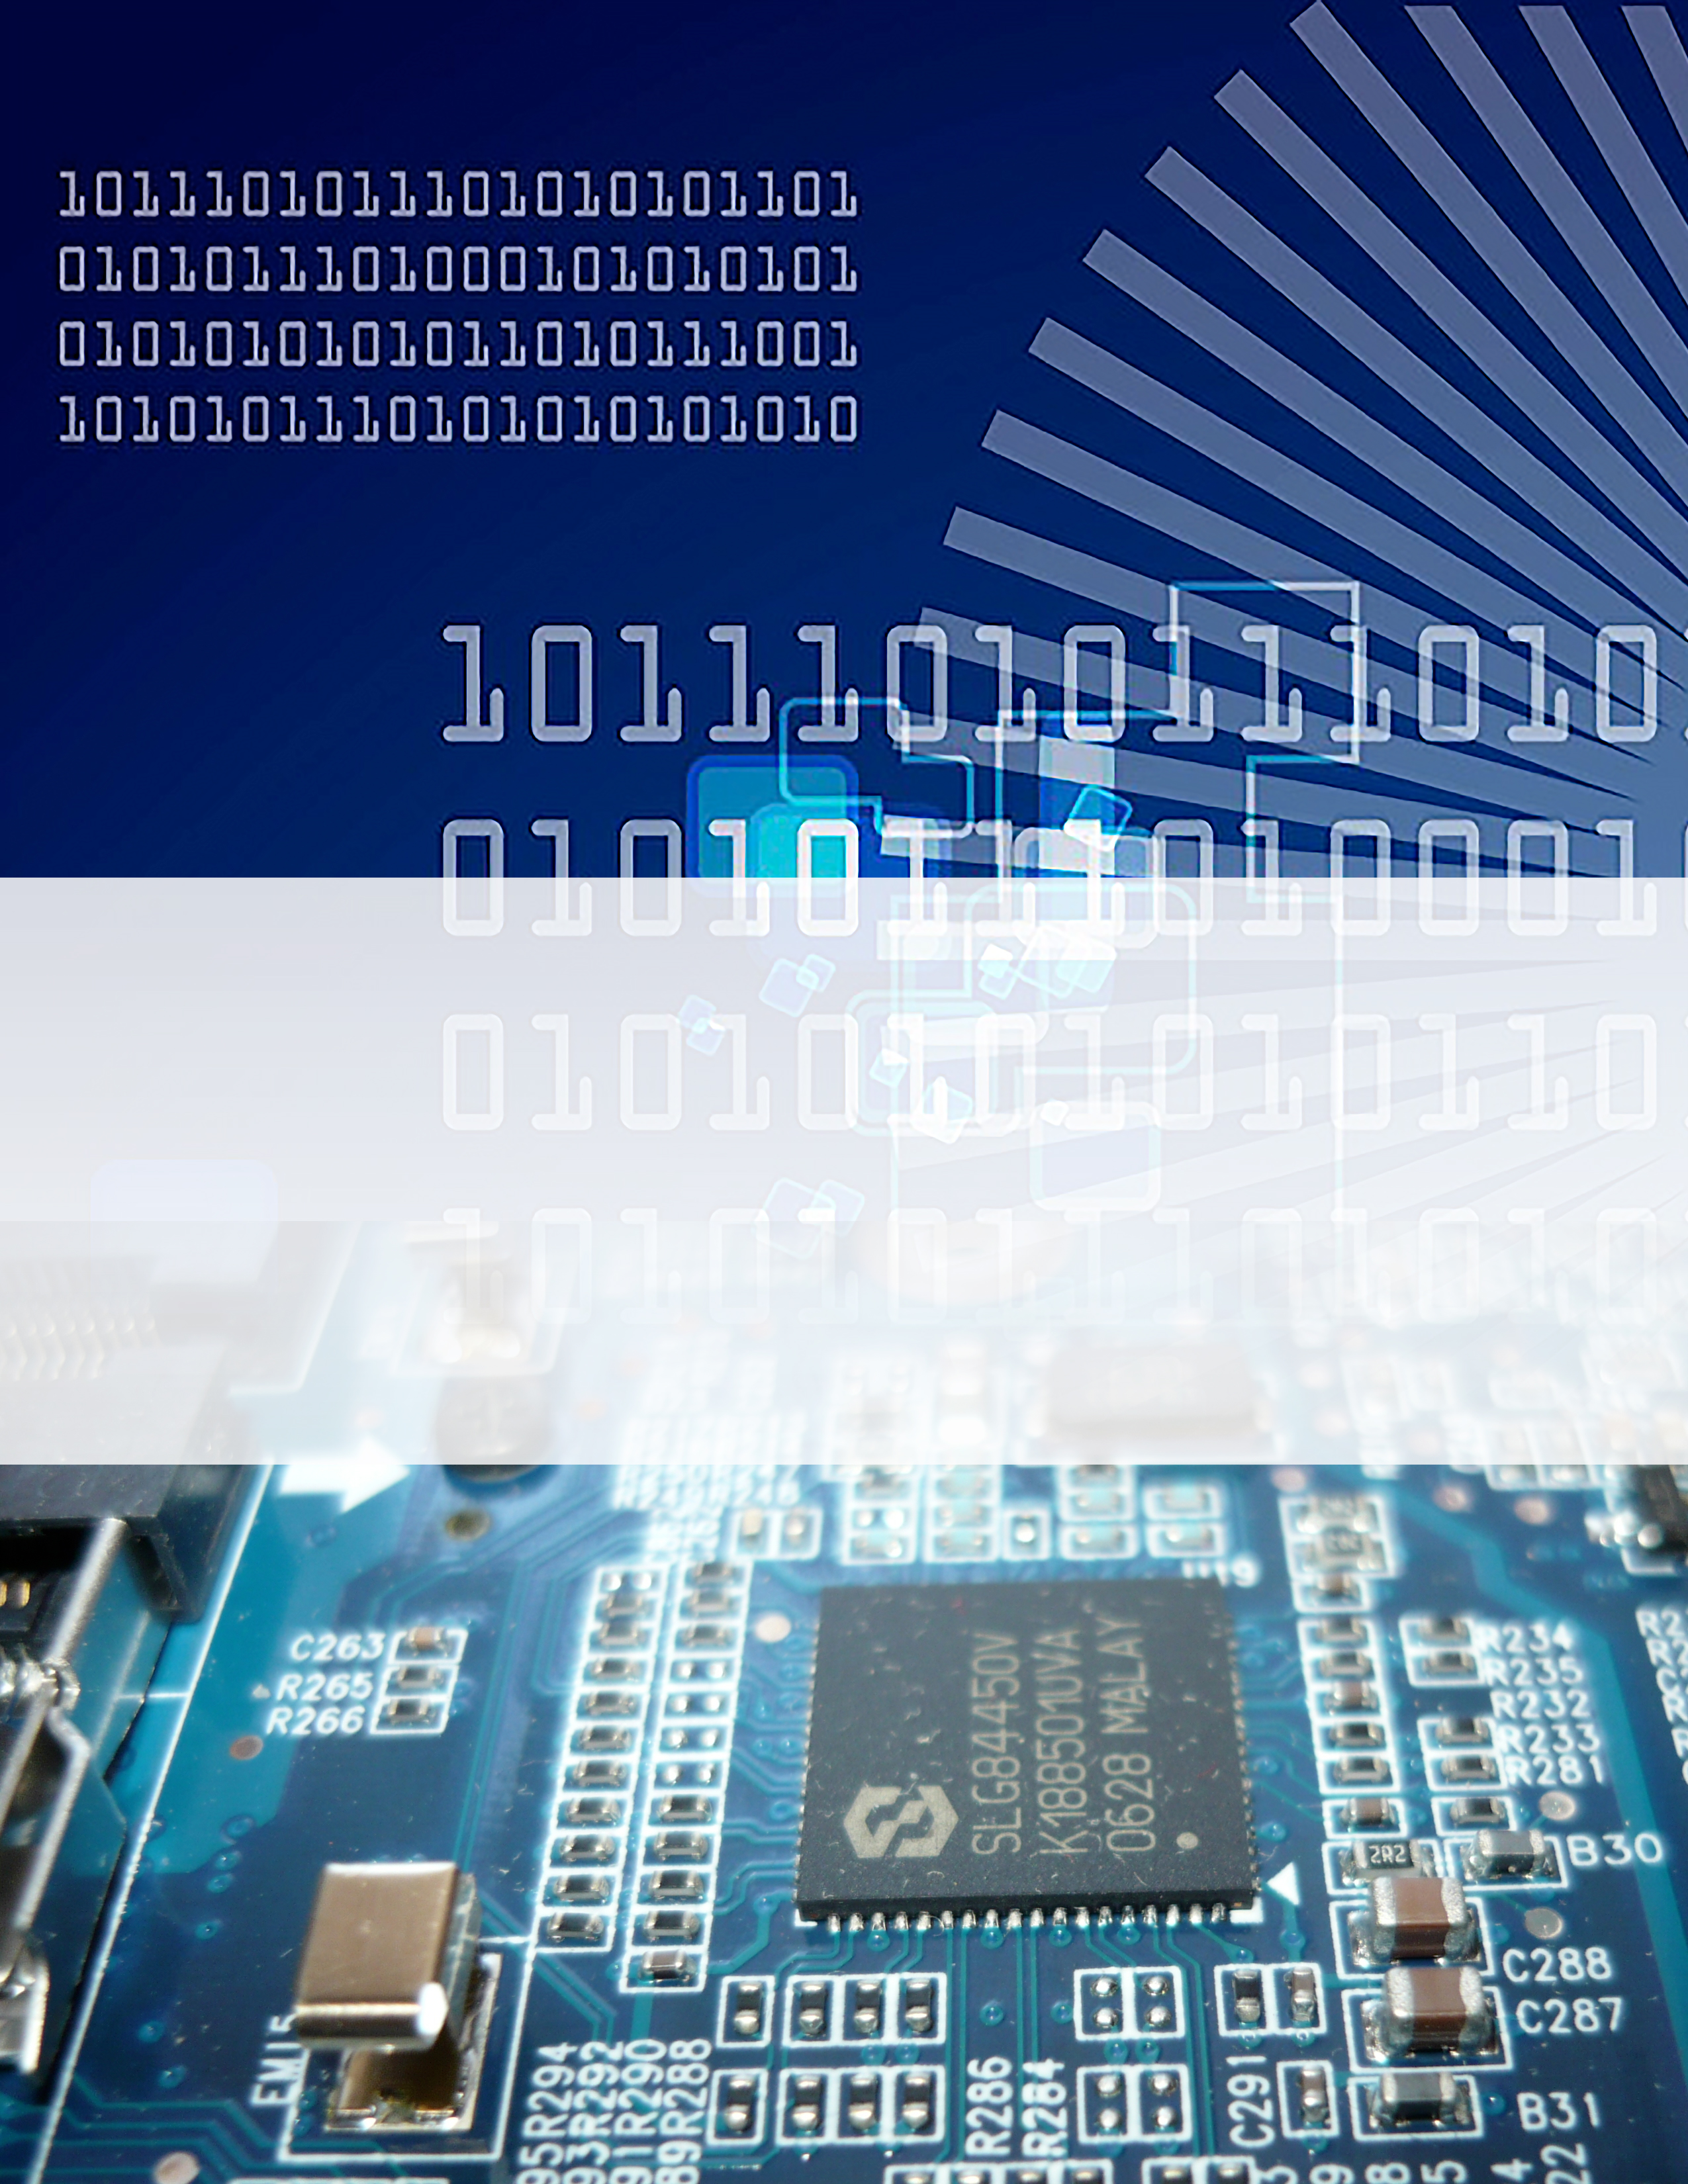
\includegraphics[height=\paperheight]{pictures/technology-backdrop.jpg}}} % Image background
%\AddToShipoutPicture*{\put(0,0){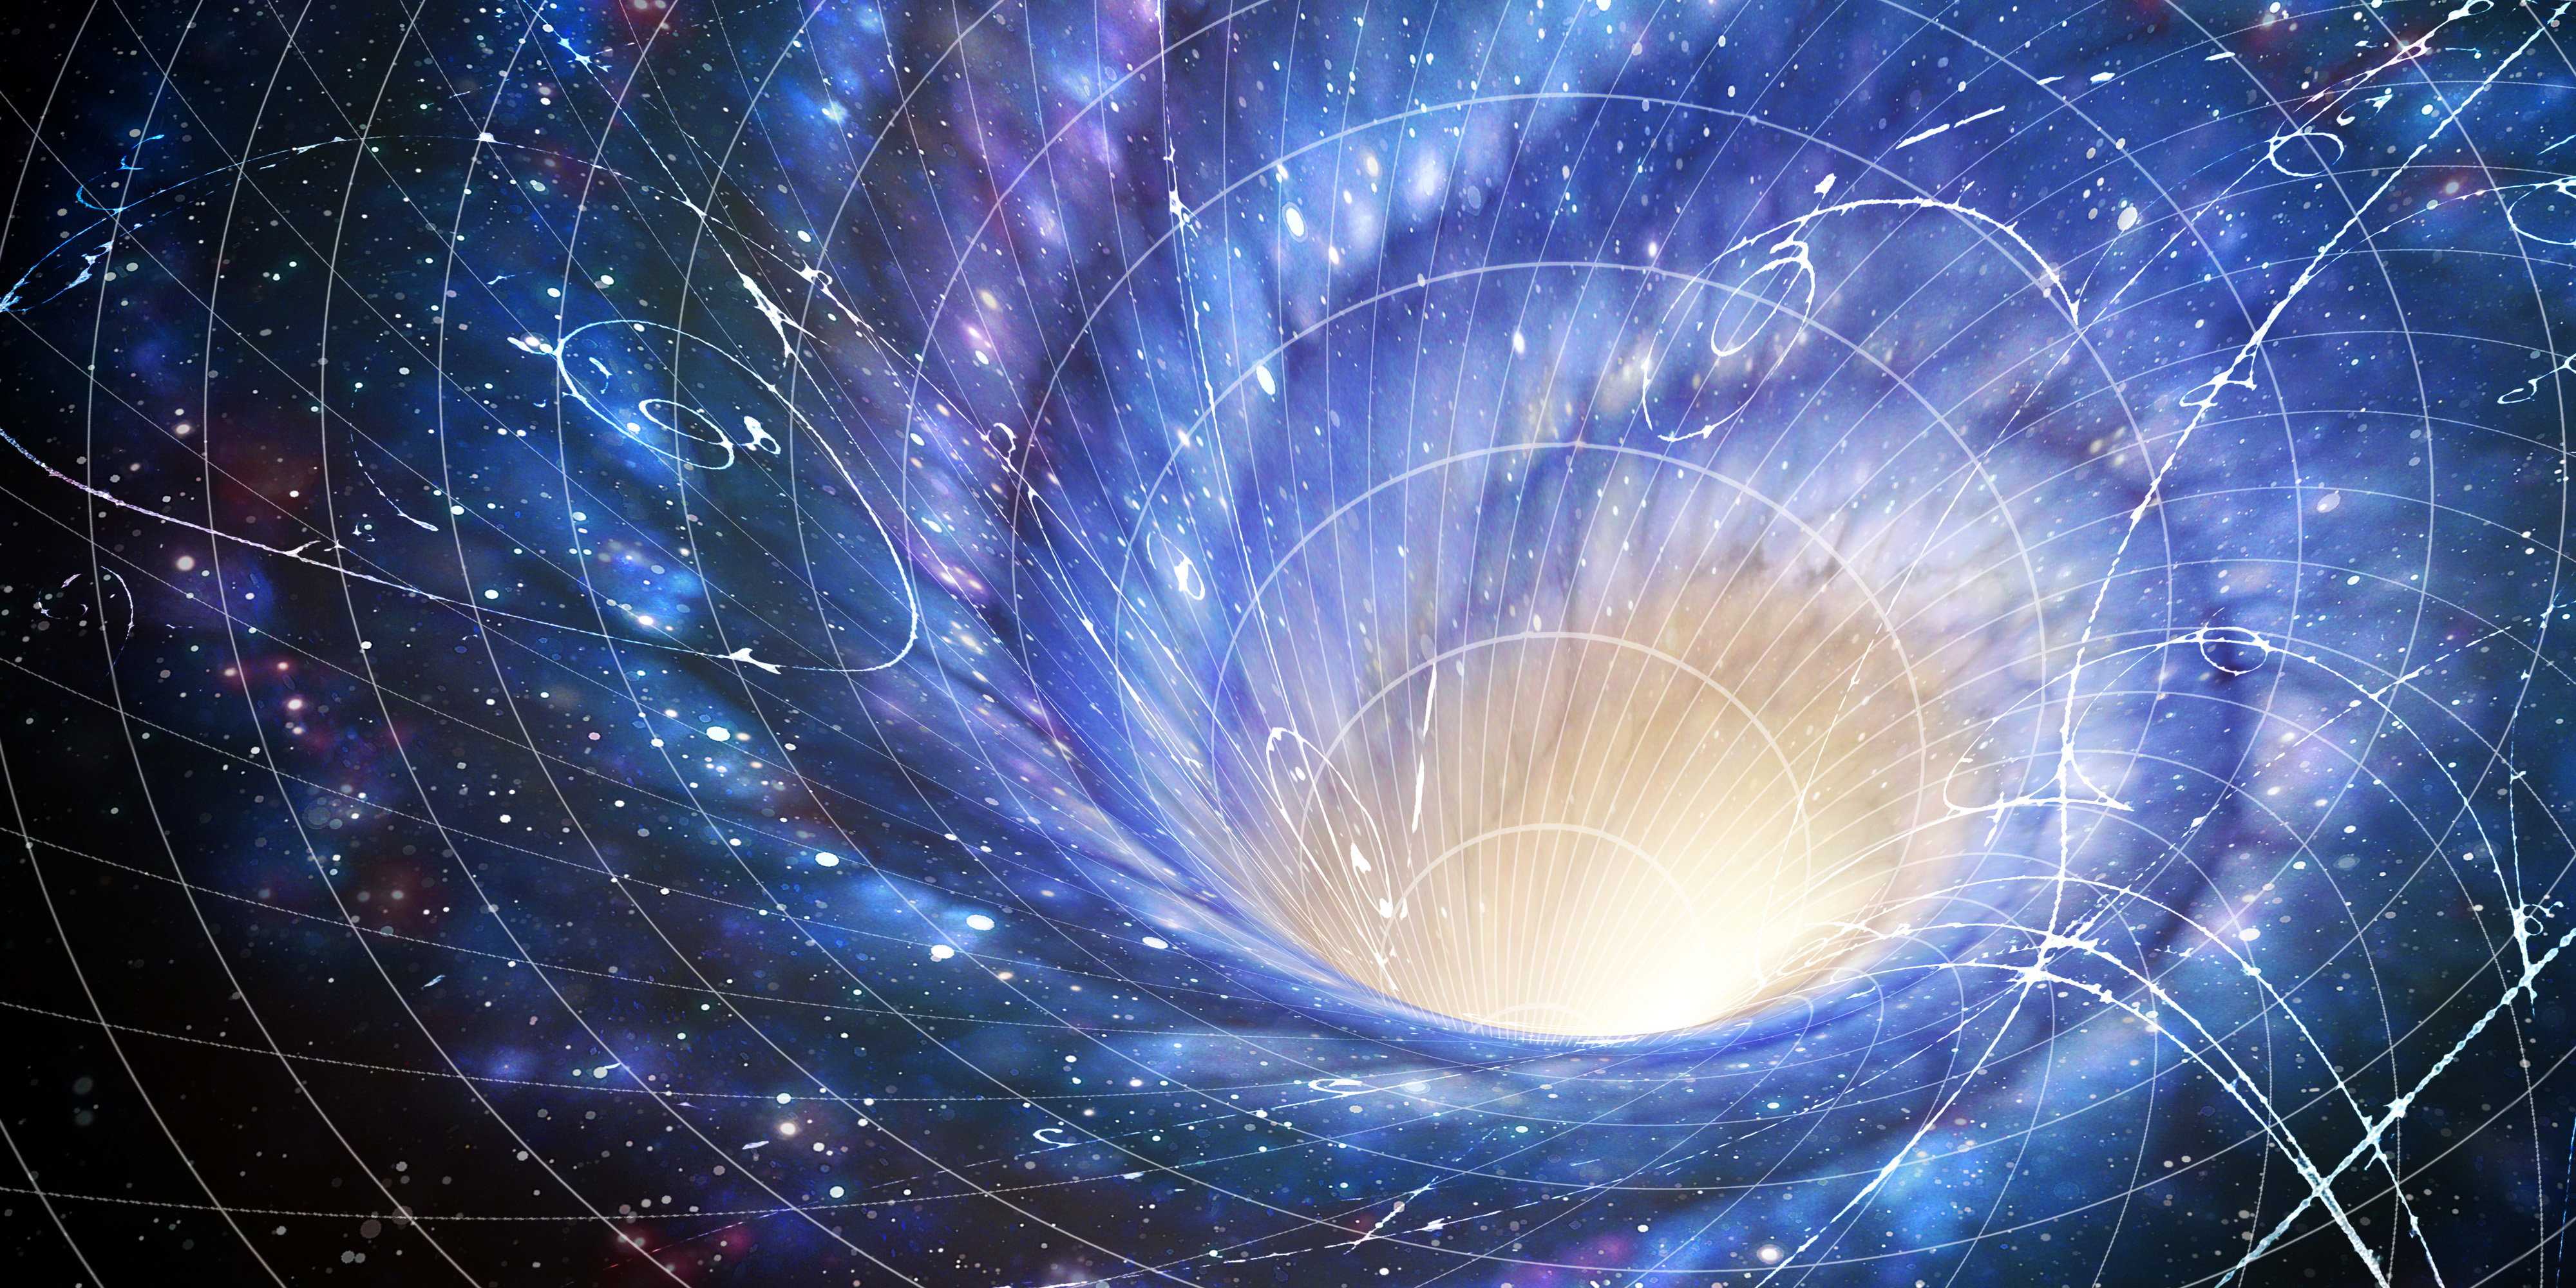
\includegraphics[scale=1.0]{galaxy_spacewarp.jpg}}}
\centering
\vspace*{7.5cm}
\par\normalfont\Huge\sffamily\selectfont
\textbf{\textcolor{black}{Case Studies Using the R Programming Language}}\\
{\normalsize \textcolor{black}{ Katherine~Bennett, Miguel~de~los~Reyes, Hannah~Gahagan, Raymond~Gao, Sophia~Hurr, Nikhil~Milind, Mridu~Nanda, Christa~Parrish, Ishaan~Rao, Margaux~Winter, Grayson~York}}\par % Author name
\endgroup

%----------------------------------------------------------------------------------------
%	COPYRIGHT PAGE
%----------------------------------------------------------------------------------------

\newpage
~\vfill
\thispagestyle{empty}

\noindent \textsc{Research in Computational Science}\medskip

\noindent \textsc{North Carolina School of Science and Mathematics, Durham, NC}\medskip % URL

\noindent This case studies manual was prepared under the direction of Mr. Robert Gotwals, faculty mentor, The North Carolina School of Science and Mathematics, Durham NC.\\
Editing and typesetting performed by Grayson~York using Tex Live 2015. \\
Code template provided by Nikhil~Milind\\
Graphics designed by Tracy Telenko, Creative Services Group, The North Carolina School of Science and Mathematics.\\
Template created by Mathias Legrand.\medskip   % License information

\noindent \textit{First release, November 2016} % Printing/edition date

\chapterimage{Pictures/ChapterHeadings/header_01.jpg} % Table of contents heading image
\pagestyle{empty} % No headers
\tableofcontents % Print the table of contents itself

%\cleardoublepage % Forces the first chapter to start on an odd page so it's on the right

\pagestyle{fancy} % Print headers again

\chapterimage{Pictures/ChapterHeadings/header_02.jpg} % Chapter heading image

\chapter*{Introduction}
\vspace{1cm}

Gotwals will write an Intro.

\chapterimage{Pictures/ChapterHeadings/header_03.jpg}

%  CONTINUING MODIFIABLE STUFF
\chapter{ANOVA}
\section{Introductory Reading}

\nomenclature{Glossary term:}{Definition}

The most common type of linear models are analysis of variance (ANOVA) and linear regression models. 
R is built to handle linear models, and as such it is easy to work with ANOVA. 
ANOVA is a statistical method used to compare two or more means. 
These values can be used to determine whether a significant correlation exists between variables. 
We will be using one-way ANOVA, which compares the means between the groups of interest, and determines whether those means are significantly different from each other. 
If one-way ANOVA returns a significant result, there are at least two group means that are significantly different from each other. 
It is important to note that ANOVA is an omnibus test statistic, meaning that although ANOVA tells the user is there is a significant difference in means, it is unable to show which means in particular differ.
ANOVA can only be used with certain types of data configurations. 
To perform ANOVA, data must have a continuous response variable and at least one categorical factor with two or more levels, in lay terms, ANOVA can only be used with numeric values that can be ordered sequentially, with a certain number of possible responses. 
(i.e. data comparing object's weights, and each new weight is a level) 
ANOVA is easier to use if data is from from approximately normally distributed populations with equal variances between factor levels, however, as R is built to work with statistics, ANOVA procedures will generally work without incident unless one or more of the distributions or variances are highly skewed.
A basic understanding of statistics how to use R is recommended before performing ANOVA. The ANOVA user will create and order factors, make box plots, and combine and stack data. 
\cite{CRANR}
The following functions will be useful in using ANOVA.
\begin{enumerate}
        \item \texttt{aov}
        \item \texttt{as.factor}
        \item \texttt{ls.str}
        \item \texttt{data.frame}
        \item \texttt{stack}
        \item \texttt{TukeyHSD}
\item \texttt{levels}
\end{enumerate}

\section{Objectives}

In this assignment, we will use ANOVA to analyze data from ELISA HIV Optical Density Readings.
ANOVA identifies the causes of variation, and sorts out the corresponding components of variation with associated degrees of freedom. 
In this case, we are interested in seeing how HIV Optical Density Readings are related to their lot. 
The type of ANOVA we are using is one-way between groups, as we are comparing one grouping (the optical density readings) to define the groups (lots). 
\setlist{before=\singlespacing,after=\singlespacing}
\singlespacing
By the end of this lesson, the reader should be able to:
\begin{enumerate}
        \item Understand the logic behind one-way analysis of variance.
        \item Perform one-way analysis of variance in R for any data. 
        \item Appropriately interpret results of analysis of variance tests.
\end{enumerate}

\subsection{ANOVA}

We will look at variances in data using R's ANOVA functions.

\subsection{Visualization}

We will also use our fitted models and our ANOVA data to create box plots and line plots.
Much of the information gleaned from ANOVA is presented via numeric such as the sum of square, degrees of freedom, and the mean.
ANOVA presents the null hypothesis that there is no difference in means of the treatments, and once this hypothesis is proven incorrect, the question arises of how the treatments differ.
The post-hoc test also allows the user to find the differences in means, and specifically categorizes the lower and upper means of the data.

Figure \ref{fig:BoxPlotOpticalDensity} shows a box plot of the data before running ANOVA or TukeyHSD.
Constructing a box plot before analyzing the data may prove helpful in deciding what kind of analysis would be preferable.

\begin{figure}%  the "H" means put it where you put this code....but that doesn't always work!
        \centering
                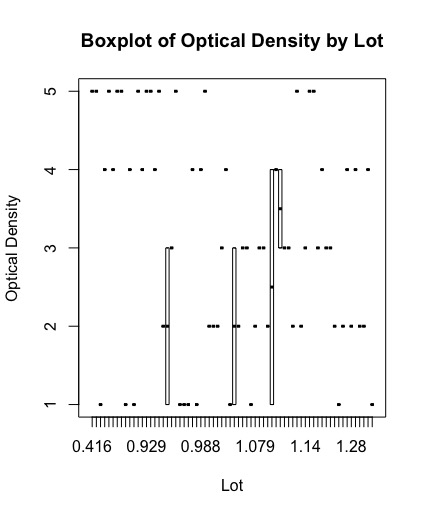
\includegraphics[width = .5\textwidth]{pictures/ANOVA/BoxPlotOpticalDensity.jpg} 
        \caption{Boxplot}
        \label{fig:BoxPlotOpticalDensity}
\end{figure}

 

\section{Building the Model}

Looking at the data set of interest for ANOVA, note that that data may be in numeric form. Use the function is.numeric to review the data. If this function prints TRUE, use the function as.factor to change data from numeric to factor. In order to make it easier to manipulate data later on, it is recommended that the factored data is renamed. 
\begin{lstlisting}
lot = as.factor(elisa$Lot)
summary(lot)
levels(as.factor(elisaOptical))
optical = (as.factor(elisa$Optical))
levels(as.factor(elisa$Run))
run = (as.factor(elisa$Run))
\end{lstlisting}
Now your factor data type is in non-numerical variables.
Each different variable of the factor is called a level.
For example, our factor type data for the lots of various ELISA HIV Optical Density Readings has five levels, 1, 2, 3, 4 and 5.
Moving on, we can make a box plot of our data, so that we can visually compare data.
Making a summary of this data allows us to look at the residuals and standard error of the plot.
As mentioned before, this type of comparison will work better with data that has a relatively normal distribution. 
Factors can also be created within factors.
We used our factor Optical to categorize and label by the density.
For each level within the main factor, create labels.
These labels will designate unordered factors.
To make this data easier to read, unordered factors should be ordered.
Choose ways to order the data that is relative to the averages in the data.
For example, some levels were Low density(below 1) and some were High density,(above 1.5) so we ordered the data starting at 0, then continuing with 1, 1.5, 2. Choose labels that reflect the data, noting that the first label will relate to the lower numbers.
Next, classify this newly ordered factor, and now label the data in lay terms. 
\begin{lstlisting}
elisa$Optical.type<-ordered(cut(elisa$Optical, c(0,1,1.5,2), labels = c("Low","M
class(elisa$Optical.type)
elisa$Optical.type
\end{lstlisting}
Note, that if you wish to remove one group of subjects (i.e. Lot 1) R will keep this removed group as a level, possibly skewing your data. Use the function drop levels to remove a selected group as a level. Rename this reconfigured data as to not overwrite your previous data. 
In order to use ANOVA, the data must be in a specific format. To properly configure data, combine the data from the two factors intended to be compared with the function data.frame. Next, stack these combined groups. Finally use this stacked data and the function aov to perform ANOVA. Make a summary of these results.
\begin{lstlisting}
finalelisa <- droplevels(newelisa)
summary(finalelisa$Lot)
Combined_Groups <- data.frame(cbind(lot,optical))
Combined_Groups
Stacked_Groups <- stack(Combined_Groups)
Stacked_Groups
Anova_Results <- aov(values ~ ind, data = Stacked_Groups)
\end{lstlisting}
This method can me used for a simple one-way ANOVA. However some data can compare multiple sets of data against each other. To do this, we can use a post-hoc test. Post-hoc tests compare outcome measurements between multiple groups. With post-hoc analysis the reader can examine differences between pairs of groups after global analysis. Use the function TukeyHSD to perform a pairwise post-hoc analysis on the ANOVA results.
\begin{lstlisting}
summary(Anova_Results)
TukeyHSD(Anova_Results)
summary(TukeyHSD(Anova_Results))
\end{lstlisting}
 \subsection{Programming Hints}
It is recommended to look at data before analysis in order to better understand the levels and attributes of data.
In addition, we recommend the use of \texttt{summary()} and the console to view the attributes of objects.
 
\section{Deliverable}

Using ANOVA, students should be able to take data with sequentially ordered number data, make a box plot, factor the data as unordered and ordered factors, configure the data such that the function aov can be performed, and perform TukeyHSD.
Using the box plot, students should be able to identify residuals, coefficients of the linear regression, and residual standard error. 
Using aov, students should be able to identify degrees of freedom, the sum of the squares, the mean of the squares, and the F ratio (the ratio of two mean square values) for their data. 

\section{Teaching Code}

Begin ANOVA by formatting the data in a \texttt{.csv} file, then uploading it to RStudio.
This script is set up to analyze publicly available data about HIV Optical density readings, but can be adapted for any properly set up data. 
As the reader works his or her way through the script, be sure to liberally comment the purpose of each command. 

\begin{lstlisting}
# Your name here
# Date
# ANOVA - ELISA HIV Optical density readings data

# Clean up and read in data
rm(list=ls())
setwd("C:/Your/Directory")
elisa = read.csv("ELISAHIV.csv")

# Create levels for lot, optical, and run
# Make sure to view/check your data
levels(as.factor(elisa$Lot))
lot=as.factor(elisa$Lot)
# etc.


# Create a boxplot showing optical density by lot
# Make sure to label your axes!
boxplot(..., ...)


# Perform a linear regression of optical density by lot
summary(lm(..., data=elisa))

# Create an ordered factor using Optical.type and verify its type
elisa$Optical.type<-ordered(...)
class(elisa$Optical.type)

# Remove 1 as a possible level
# Note: even if you eliminate a group of subjects (ex. 1),
# because it's a factor, R keeps 1 as a possible level for lot

# Use droplevels() to remove 1

# Create stacked results to run aov()

# Run TukeyHSD on the ANOVA results

\end{lstlisting}

\section{Example Student Code}
\begin{lstlisting}
# KEY
# ANOVA - ELISA HIV Optical density readings data

# Clean up and read in data
rm(list=ls())
setwd("C:/Example/Code")
elisa = read.csv("ELISAHIV.csv")

# Look at variables and create levels
ls.str(elisa)
levels(as.factor(elisa$Lot))
lot=as.factor(elisa$Lot)
summary(lot)
levels(as.factor(elisa$Optical))
optical = (as.factor(elisa$Optical))
levels(as.factor(elisa$Run))
run = (as.factor(elisa$Run))

# Create a boxplot
boxplot(elisa$Lot~elisa$Optical, xlab="Lot", ylab="Optical Density", 
    main="Boxplot of Optical Density by Lot")
summary(lm(elisa$Optical~elisa$Lot, data=elisa))

# Perform regression
summary(optical)
elisa$Optical.type<-ordered(cut(elisa$Optical, c(0,1,1.5,2),
    labels=c("Low","Medium","High")))
class(elisa$Optical.type)
elisa$Optical.type

# Remove 1 as a level
# We've verified that optical is an ordered factor
# Note: even if you eliminate a group of subjects (ex. 1),
# because it's a factor, R keeps 1 as a possible level for lot
newelisa <- elisa[1:2,]
summary(newelisa$Lot)
# We remove 1 as a possible level using droplevels()
finalelisa <-droplevels(newelisa)

# We create stacked results to run aov()
summary(finalelisa$Lot)
Combined_Groups <- data.frame(cbind(lot,optical))
Combined_Groups
Stacked_Groups <- stack(Combined_Groups)
Stacked_Groups
Anova_Results <- aov(values ~ ind, data = Stacked_Groups)
summary(Anova_Results)

# We also run TukeyHSD on the ANOVA results
TukeyHSD(Anova_Results)
summary(TukeyHSD(Anova_Results))
\end{lstlisting}

\section{Further Readings}

\begin{enumerate}
        \item Seefeld, Kim and Linder, Ernst. \emph{Statistics Using R with Biological Examples}, University of New Hampshire, Durham, NH Department of Mathematics and Statistics(2007)
        \item Julian J. Faraway. \emph{Practical Regression and Anova using R}, University of Michigan, (2002)
\end{enumerate}


\chapterimage{Pictures/ChapterHeadings/header_04.jpg}

\chapter{Neural Networks}
\section{Introduction to Neural Networks}

In the field of computational research, the use of computers is generally restricted to discreet, exact commands that are meant to be executed in a certain manner, which  provide the computational power required for complex calculations.
In contrast, neural networks are an example of machine learning (ML), wherein the machine is capable of learning behavior or interpreting patterns from a given data set.
The field of predictive analysis uses this paradigm of computational interpretation.
For example, it is extremely challenging to develop a system that is purely programmed to recognize handwriting.
Yet, computers at the United States Postal Service are able to decipher human words and reroute letters and packages without the need for humans.
These computers contain a neural network that has been trained to recognize handwriting and predict characters as they appear on mail. \cite{nielsen} 

\begin{figure}[htbp!]
   \centering
   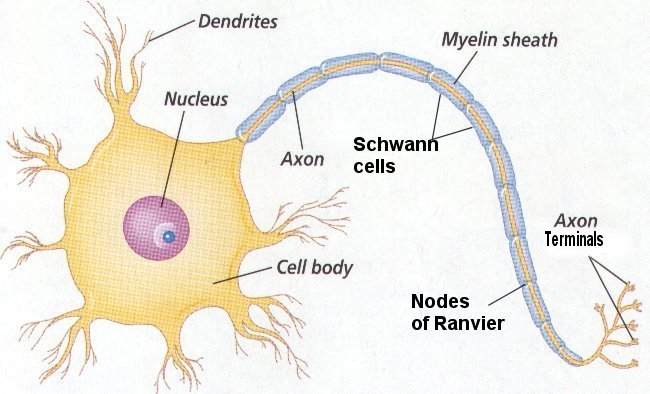
\includegraphics[scale=0.75]{pictures/NeuralNetworks/neuron.jpg} 
   \caption{The Parts of an Anatomical Neuron}
   \label{fig:neuron}
\end{figure}

Neural networks were designed using the human brain as an inspiration.
The neural network is composed of perceptrons, which are similar to the smallest functional units of the brain: the neuron.
Neurons act as the wiring of the brain by passing along signals that they receive to other neurons.
When a neuron communicates with another neuron, it uses neurotransmitters to either increase or decrease the probability of the next neuron firing.
Thus, a neuron can be excitatory (increases the chance of the next neuron firing) or inhibitory (decreases the chance of the next neuron firing).
Similarly, neural networks utilize perceptrons that can receive multiple inputs and produce a single output.
The inputs are binary values ($0$ or $1$), and affect the perceptron differently depending on their excitatory or inhibitory ability.
The amount of excitation or inhibition is captured by weights, or values that the inputs are multiplied by.
Finally, the aggregate sum of these inputs and their weights is used to calculate if the perceptron in question will fire an output to the next layer of perceptrons. 

\begin{figure}[htbp!]
    \centering
    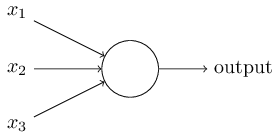
\includegraphics[scale=1.0]{pictures/NeuralNetworks/sigmoidNeuron.png}
        \caption{A neuron in a neural network, with binary inputs $x_1$, $x_2$, and $x_3$.}
    \label{fig:sigmoidNeuron}
\end{figure}

Neurons that only utilize binary inputs, however, are not efficient in learning.
For example, neurons in the brain release different amount of neurotransmitters to indicate different levels of excitation.
Similarly, most modern neural networks generate an output that is between $0$ and $1$, inclusive.
This type of function is known as the sigmoid function, and the resulting neuron is known as the sigmoid neuron. 

\subsection{Neural Networks with Sigmoid Neurons}

With practice, humans can arrange sigmoid neurons to generate a functional unit that can take inputs and produce a certain computational output.
Functionally, sigmoid neurons act as NAND gates, which are universal to computational procedures.
However, the true value of the neural network lies in data and input values that do not have any discernible pattern.
In such cases, neural networks are capable of learning patterns by themselves.
Therefore, neural networks can be trained with an initial data set, after which they can predict the output values of new information.
Although a single sigmoid neurons can be trained, it is not adequate to use such a unit to capture the entirety of complex patterns found in data sets.
Rather, a network of sigmoid neurons is created to assess input values and generate proper outputs.
Neural networks are most often arranged in layers.
The first layer is known as the input layer, whilst the last layer is known as the output layer.
All the neural layers in the middle are known as hidden layers. 
\begin{figure}[htbp!]
    \centering
    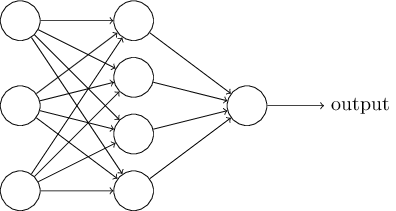
\includegraphics[scale=0.75]{pictures/NeuralNetworks/neuralNetwork.png}
        \caption{A neural network with three layers: an input layer, a hidden layer, and an output layer.}
    \label{fig:neuralNetwork}
\end{figure}
The sample neural network shown in figure \ref{fig:neuralNetwork} takes four inputs in the first layer and produces a singular output.
Since all the components involved are sigmoid neurons, the value of the output of the neural network can take any value between 0 and 1. 

\subsection{Training in a Neural Network}

In general, every sigmoid neuron has a certain set of inputs $X=\{x_1, x_2, \hdots , x_n\}$.
Each input is associated with a weight, or the amount of excitation or inhibition each input causes, which are expressed as the weight set $W=\{w_1, w_2, \hdots , w_n\}$.
The value of the previous inputs is also influenced by a neuron-specific bias $b$, which acts as a value of how reactive the neuron is to the inputs.
Finally, the sigmoid neuron produces an output $O$ between $0$ and $1$ depending on the influence of previous inputs as follows:

\begin{gather*}
    \sigma (x)=\frac{1}{1+e^{-x}}\\
    O(W, X)=\sigma \left(\sum_{i}^{n} w_{i}x_{i} + b\right)\\
    O(W, X)=\sigma \left(W\cdot X + b\right)\\
    O(W, X)=\frac{1}{1+e^{-W\cdot X - b}}
\end{gather*}

Therefore, by computing the dot product of set $W$ and set $X$, offsetting the dot product by the neural bias, and then passing that value through the sigmoid function, we generate an output between 0 and 1.
If the sigmoid neuron in question is part of a hidden layer, it will pass on its output to other neurons in the next lay. 

To train a network, we begin with a neural network that is set up with well-chosen (but random) weights and begin sending input values through it.
The output is then compared to the value we were expecting, and computational corrections are made in increments to the weights and biases in the neural network using gradient descent algorithms.
Over time, the neural network becomes more accurate and has the ability to predict future output values from input values.

\subsection{Measuring Predictive Error}

To train our neural network computationally, we need to develop a cost function, that quantifies the amount of training our neural network has undergone.
That is, this function has to return a value that quanitifies the difference between prediction and reality.
During training, every predicted value is compared to the actual value of the data through subtraction and squared.
Thus, for a prediction $y$ and actual value $\hat y$.

\[
C(y,\hat y)=(\hat y - y)^2
\]

The cost function is computed for every data point used to train the neural network.
The overall error of the neural network is simply the average of all the cost function values for every data point that was used to train the network.
However, since we are squaring the cost function, we divide the average by 2 to decrease the severity of predictive error.
This error function is most commonly known as the Mean-Squared Error function, and is predominantly used to train neural networks.
For a set of predictions $Y=\{y_1,y_2,\hdots,y_n\}$ and a set of actual values $\hat Y=\{\hat y_1,\hat y_2,\hdots,\hat y_n\}$:

\begin{gather*}
J(Y,\hat Y)=\sum_{i=0}^{n} \frac{C(y_i,\hat y_i)}{2n} \\
J(Y,\hat Y)=\sum_{i=0}^{n} \frac{(\hat y_i - y_i)^2}{2n}
\end{gather*}

\section{Installation}

The neuralnet package can be found at \url{https://cran.r-project.org/web/packages/neuralnet/index.html}.
Download the package that works for your operating system and CPU architecture.
The following code can be used to install the package from the R command line.
This example illustrates the installation of a windows system binary file.
However, all other installations will also be the same, with \texttt{FILE\_PATH} leading to the package downloads.
Alternatively, a script file can be generated to install the neuralnet package. 
\begin{figure}[htbp!]
\caption{Code for Windows}
\begin{lstlisting}
install.packages("FILE_PATH.zip", repos=NULL)
package 'neuralnet' successfully unpacked with MD5 sums checked
library(neuralnet)
\end{lstlisting}
\end{figure}

\begin{figure}[htbp!]
\caption{Code for Mac / OSX}
\begin{lstlisting}
install.packages("FILE_PATH.tgz")
package 'neuralnet' successfully unpacked with MD5 sums checked
library(neuralnet)
\end{lstlisting}
\end{figure}

Note that safari automatically decompresses \texttt{.tgz} files to tar files, and this will cause errors when running the above code.
The installation may throw a warning reminding the user that the package may be out-of-date when compared to the R version being used. 

\section{Objectives of Case Study}

There are multiple objectives that the student must accomplish over the course of this neural networks case study.
\begin{enumerate}
\item Understand neural networks, their functional units, and their overall purpose in Machine Learning.
It is important to understand how neural networks work, beginning from an understanding of sigmoid neurons and culminating in an overall appreciation for the function of neural networks in predictive analysis.
\item Have the ability to prepare data for use in neural networks in R.
This objective includes the ability to identify and remove rows with empty data, normalizing the data to allow for learning over a smaller number of iterations, and fitting data curves to create the predictive function.
\item Be able to implement the neuralnet package in R.
An understanding of the functionality that the neuralnet package provides, including creating the neural network, training it with a data set, and using it for predictive analysis, is imperative to this objective.
\item Perform cross-validation on the neural network to confirm understand its learning progress.
This involves using statistical measures to see how the neural network is functioning during training and prediction.
\end{enumerate}
\section{Case Study - Boston Housing Database}

The Boston Housing Database is a databaase that contains the housing data from the boston area.
It contains data on housing sales, including the area of the house sold, the location of the house, and other price-determining factors.

\subsection{Loading and Separating the Data}

Create a R script file and enter the following code. This code will set up the environment for the neural network. We load the data into our scripting environment, modify it to fit the neuralnet package, and split it into a training and testing dataset. 
\begin{lstlisting}
# Name:     neural.R
# Author:   First Last
# Date:     Month Date Year

# Load necessary libraries into R
library(neuralnet) # Contains the neuralnet package
library(MASS)      # Contains the database we will use

# Clear the current environmental variables
rm(list=ls())

# We set the seed for the random generator
# We use random data values for training and for testing
# Use this seed to replicate the results in this chapter
set.seed(500)

# Import the database into R from the MASS library
data <- Boston

# Define the number of neurons in each hidden layer
# The input layer depends on the number of columns in the data frame
# The output layer depends on variables we ask the network to predict
hiddenLayers = c(5, 3)
\end{lstlisting}

Unfortunately, the neuralnet package cannot handle NULL values in the data.
Therefore, we must remove such extraneous data from the dataset.

\begin{lstlisting}
# Unlike most R libraries, neuralnet is unable to parse NA values
# We check for NA values in the data set and print their amount
# If we have rows with missing data, we will have to remove them
apply(data, 2, function(x) sum(is.na(x)))
\end{lstlisting}

We will use 75\% of the data to train the network and 25\% to test the efficacy of the neural network.
We split the dataset using the following code.

\begin{lstlisting}
# Generate a list of indices that are randomly sampled
# The indices point to rows in the data
# 75 percent of the data set indices is selected in this list
index <- sample(1:nrow(data), round(0.75 * nrow(data)))

# The training data set is composed of 75 percent of the test data
train <- data[index,]

# The testing data set is composed of 25 percent of the test data
test <- data[-index,]
\end{lstlisting}

\subsection{Linear Model for Comparison}

First, we run the data through a simple linear model to see how well a linearly scaled system can predict the value of interest in the data set.
Our data frame is constructed so that the last column, named \verb|data$medv|, is what is predicted. Every other column is the value of a pixel in the image.

\begin{lstlisting}
# Create a regression line using prog as the prognostic variable
lm.fit <- glm(medv~., data=train)
# Print the summary of our fit
summary(lm.fit)
# Predict values using the fit and the testing data set
lm.pr <- predict(lm.fit, test)
# Calculate the Mean-Square Error of the linear model
lm.MSE <- sum((lm.pr - test$medv)^2) / nrow(test)
\end{lstlisting}

\subsection{Neural Network Setup and Execution}

We will compare the linear model to the neural network graphically after generating results from the neural network.
We now work to set up the data for the neural network.
Neural networks generally do not work well with non-uniform distributions of data.
Therefore, we will scale every column to distribute the values correctly.
When we scale the data set, we will lose the true values.
Therefore, it is important to ''unscale'' the data once we generate output from the network.

\begin{lstlisting}
# Create a list of maximums from each data column
maxs <- apply(data, 2, max)
# Create a list of minimums from each data column
mins <- apply(data, 2, min)

# Scale the values in each column to its respective limits
scaled <- as.data.frame(scale(data, center=mins, scale=maxs - mins))

# Redefine a training data set using the scaled values
train_ <- scaled[index,]
# Redefine a testing data set using the scaled values
test_ <- scaled[-index,]
\end{lstlisting}

At this point, we can generate a neural network and execute it.
We begin by constructing a rule for the neural network to follow.
This rule simply describes the output variables and the input variables that are thought to influence the output. 

\begin{lstlisting}
# Every column affects the prognostic variable
# We extract the name of every column in the data set
n <- names(train_)

# Using the normal fit construct (prog ~) does not work in this package
# Instead, we generate the command using the following code
# Will generate something like this: prog ~ c1 + c2 + c3 + ...
f <- as.formula(paste("medv ~", paste(n[!n %in% "medv"], collapse=" + ")))

# The following code will generate the neural network
# This step can take some time
nn <- neuralnet(f, data=train_, hidden=hiddenLayers, linear.output=T)

# We can plot the neural network to view its structure
plot(nn)
\end{lstlisting}

Just like the linear model that we use to compare, we will calculate the Mean-Squared Error of the neural network.
For this, we extract the predictions of the neural network and ''unscale'' them. 

\begin{lstlisting}
# Compute predictions from our neural network
nn.pr_ <- compute(nn, test_[,1:13])

# Unscale the data output from the neural network
nn.pr <- nn.pr_$net.result * (max(data$medv) - min(data$medv)) + min(data$medv)
test.r <- (test_$medv) * (max(data$medv) - min(data$medv)) + min(data$medv)

# Root Mean Square Error computation for the neural network
nn.MSE <- sum((test.r - nn.pr)^2) / nrow(test_)
\end{lstlisting}

\subsection{Graphical Representation}

Now, we simply use descriptive and graphical methods to highlight the difference between a linear fit model and the neural network.

\begin{lstlisting}
# A higher number will suggest a lower correlation between the prediction and reality
print(paste(lm.MSE, nn.MSE))

# Set up a plot to hold two graphs
par(mfrow=c(1, 2))

# Plot the neural network's real vs. predicted values
plot(test$medv, nn.pr, col="red", main="Real vs. Predicted NN", pch=18, cex=0.7, xlab="Actual Value", ylab="Neural Network")
# Generate a line and legend for the plot
abline(0, 1, lwd=2)
legend("bottomright", legend="LM", pch=18, col="red", bty="n", cex=0.95)

# Plot the linear model's real vs. predicted values
plot(test$prog, lm.pr, col="blue", main="Real vs. Predicted LM", pch=18, cex=0.7, xlab="Actual Value", ylab="Linear Fit")
# Generate a line and legend for the plot
abline(0, 1, lwd=2)
legend("bottomright", legend="LM", pch=18, col="blue", bty="n", cex=0.95)

# Generate a plot with both scatter plots for better comparison
par(mfrow=c(1, 1))
plot(test$medv, nn.pr, col="red", main="Real vs. Predicted", pch=18, cex=0.7, xlab="Actual Value", ylab="Predicted Value")
points(test$medv, lm.pr, col="blue", pch=18, cex=0.7)
abline(0, 1, lwd=2)
legend("bottomright", legend=c("NN", "LM"), pch=18, col=c("red", "blue"))
\end{lstlisting}

A proper execution of the neural network should show that the Mean-Squared Error of the generalized linear fit model is much higher than that of the neural network. Furthermore, the graphs should portray a tighter clustering of the neural network data points around the linear fit. 

\section{Student Assignment - Temperature Dataset} 

The student is tasked with creating a neural network that interprets a dataset that contains the monthly temperatures from January to November over multiple years. The goal of the network is to predict the temperatures of the month of December. The following code should be used to parse the data:

\begin{lstlisting}
# Name:         neuralStudent.R
# Author:       First Last
# Date:         Month Date Year

### PARSING ###

monthlyavg <- c(-4.07, -1.75, 2.17, 8.06, 13.90, 18.77, 21.50, 20.50, 16.27, 9.74, 2.79, -2.36)
rawdata <- read.csv("berkeleyusdata.txt", header = FALSE)
tempdevs <- rawdata$V4
temps <- rawdata$V4 + monthlyavg
months <- rawdata$V3
mat <- matrix(temps,ncol=12)
datafornnet <- data.frame(mat)
colnames(datafornnet) <- c("Jan","Feb","Mar","Apr","May","Jun","Jul","Aug","Sep","Oct","Nov","Prog")
data <- datafornnet
rm(monthlyavg, rawdata, tempdevs, temps, months, mat, datafornnet)
\end{lstlisting}

Thus, the data set is stored in a variable called \verb|data|. The neural network can now be built by the students. The name of the variable being predicted is \verb|Prog|. 

\begin{lstlisting}
# Clear environment variables
rm(list = ls())

# Import the appropriate libraries
library(neuralnet)

# We do not need to set a seed
# We can if the pseudo-random system creates better results
# set.seed(500)

# Vary the number of neurons in the hidden layers to get better results
# This is an example a student may use
hiddenLayers = c(5, 3)

# Ensure that the data has no NaN values
apply(data, 2, function(x) sum(is.na(x)))

# Split the data into 75% and 25%
# One dataset is for training and the other is for testing
index <- sample(1:nrow(data), round(0.75 * nrow(data)))
train <- data[index,]
test <- data[-index,]

# Create a generalized linear fit to compare with the neural network
lm.fit <- glm(Prog~., data=train)
# Print the summary of the fit
summary(lm.fit)
# Predict values using the fit
lm.pr <- predict(lm.fit, test)
# Calculate the Mean-Squared Error of the model
lm.MSE <- sum((lm.pr - test$Prog)^2) / nrow(test)

# Calculate mins and maxes for scaling
maxs <- apply(data, 2, max)
mins <- apply(data, 2, min)
# Scale using the range of the data
scaled <- as.data.frame(scale(data, center=mins, scale=maxs-mins))
# Create the scaled training and test data sets
train_ <- scaled[index,]
test_ <- scaled[-index,]

# Create the neural network
n <- names(train_)
f <- as.formula(paste("Prog ~", paste(n[!n %in% "Prog"], collapse=" + ")))
nn <- neuralnet(f, data=train_, hidden=hiddenLayers, liner.output=T)
plot(nn)

# Calculate the scaled predictions and errors
nn.pr_ <- compute(nn, test_[,1:11])
nn.pr <- nn.pr_$net.result * (max(data$Prog) - min(data$Prog)) + min(data$Prog)
test.r <- (test_$Prog) * (max(data$Prog) - min(data$Prog)) + min(data$Prog)
nn.MSE <- sum((test.r - nn.pr)^2) / nrow(test_)

# Print the resulting mean-squared errors
print(paste(lm.MSE, nn.MSE))

# Generate the graphics for displaying data
par(mfrow=c(1,2))
plot(test$Prog, nn.pr, col="red", main="Real vs. Predicted NN", pch=18, cex=0.7, xlab="Actual Value", ylab="Neural Network")
abline(0, 1, lwd=2)
legend("bottomright", legend="LM", pch=18, col="red", bty="n", cex=0.95)
plot(test$Prog, lm.pr, col="blue", main="Real vs. Predicted LM", pch=18, cex=0.7, xlab="Actual Value", ylab="Linear Fit")
abline(0, 1, lwd=2)
legend("bottomright", legend="LM", pch=18, col="blue", bty="n", cex=0.95)
par(mfrow=c(1,1))
plot(test$Prog, nn.pr, col="red", main="Real vs. Predicted", pch=18, cex=0.7, xlab="Actual Value", ylab="Predicted Value")
points(test$Prog, lm.pr, col="blue", pch=18, cex=0.7)
abline(0, 1, lwd=2)
legend("bottomright", legend=c("NN", "LM"), pch=18, col=c("red", "blue"))
\end{lstlisting}

\section{Downloading The Dataset}

Download the file located at \url{https://github.com/nosyarg/textbookdata/blob/master/berkeleyusdata.txt}.
This data comes from the Berkeley Earth Project.


\chapterimage{Pictures/ChapterHeadings/header_05.jpg}

\chapter{Shiny Package Tutorial}
\section{Introductory Reading}

Shiny is a package used in R, that enables the user to easily create interactive applications.
Shiny can be used to create both simple histograms of disease data or interactive maps of the crime rate in different cities.
With Shiny the possibilities are endless.
In this lab, you will learn how to create a basic Shiny application. 
\begin{figure}
   \centering
   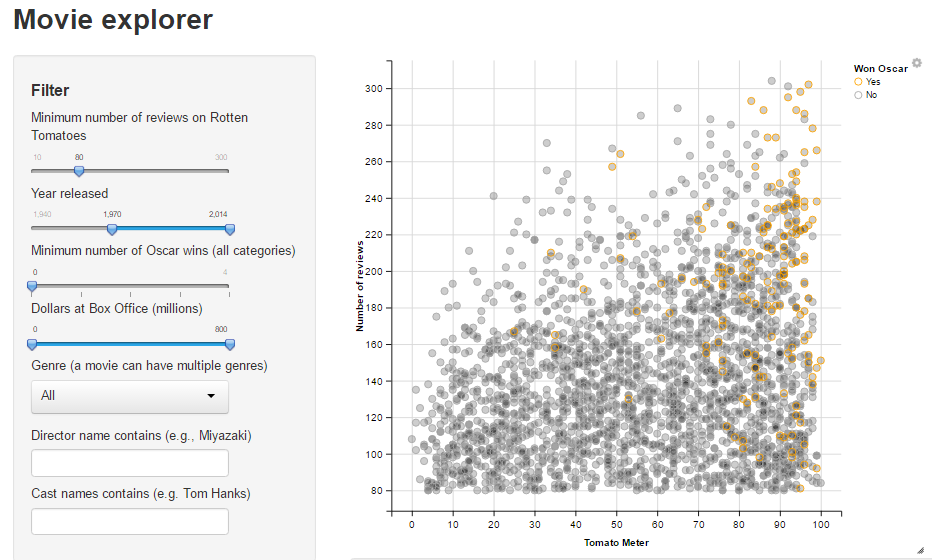
\includegraphics[width = 0.5\textwidth]{pictures/shiny/shiny.PNG} 
   \caption{Sample Shiny app}
   \label{fig:sampleapp}
\end{figure}
\noindent Look at the picture in Figure \ref{fig:sampleapp}.
\cite{gallery} This is a sample Shiny app depicting a graph of many famous movies.
The graph plots movies based on their rating and the number of reviews it has on Rotten Tomatoes.
On the left of the graph you find various inputs, such as Oscars and genres, that can customize the output of the graph.
These are the basic components of a Shiny app: inputs and outputs.     
Here are some examples of Shiny input functions:
\begin{itemize}
    \item \texttt{checkboxInput}: a single check box
    \item \texttt{dateInput}: a calendar
    \item \texttt{fileInput}: file upload
    \item \texttt{numericInput}: enter number
    \item \texttt{radioButtons}: set of radio buttons
    \item \texttt{selectInput}: box with multiple choices
    \item \texttt{sliderInput}: a slider bar
    \item \texttt{textInput}: enter text
\end{itemize}
\noindent The users of a Shiny app will interact solely with the inputs that you, the developer, will allow them to.
The above inputs can collect various types of data input from the user, to determine many different types of outputs.
Here are some of the output functions in Shiny:
\begin{itemize}
    \item \texttt{imageOutput}: creates image
    \item \texttt{plotOutput}: creates a plot
    \item \texttt{tableOutput}: creates a table
    \item \texttt{textOutput}: creates text
\end{itemize}

Understanding how inputs and outputs relate to each other is a key requirement for developing a Shiny app.
In the model students will create today, the inputs will be dropdown boxes (\texttt{selectInput}) and the output will be a simple scatterplot (\texttt{plotOutput}). 

\section{Objectives}
Students will be expected to learn the basic components of a Shiny App.
Students will create their own application after learning the fundamentals of the package.
This application will illustrate the progression of Olympic swimming medalists' times since the modern Olympics began. 
\begin{itemize}
\item By the end of this lesson the student will understand the various parts of a Shiny app, while building a simple population prediction application.
\item Students will also be able to create their own Shiny apps from scratch, and will be expected to create a Shiny app displaying Olympic swimming times over various events and years.
\end{itemize}
\section{Building the Model}

Shiny applications have a wide variety of uses. Today students will learn how to create a basic population prediction model. 

\noindent To begin the application, open a new R script file in RStudio, clear the environment, set a working directory, and import the libraries necessary for this project.
To clear the environment and set a directory use the following functions.
Make sure you set a directory on your computer that the dataset is located in. 

\begin{lstlisting}[language = R]
rm(list=ls())
setwd("C:/Users/Ishaan/Documents/NCSSM 2015-2016")
\end{lstlisting}

\noindent The libraries are as follows:

\begin{lstlisting}[language = R]
library(ggplot2)
library(scales)
library(ggmap)
library(dplyr)
library(car)
library(gcookbook)
library(shiny)
\end{lstlisting}


\noindent If you don't have one of these libraries installed on your computer, you can simply type 
\begin{lstlisting}[language = R]
install.packages("insertlibraryname") 
\end{lstlisting}
in the console to download them. 

\noindent Next, we need to import the dataset of all the population data in NC for the next five years into a variable of your choice (I used \texttt{popData}).
This can be done with the read \texttt{.csv} function.
Make sure the data file is in directory you specified above. 

\begin{lstlisting}[language = R]
popData <- read.csv("Population.csv")
\end{lstlisting}
Shiny applications have two components: a user-interface definition and a server script.
The user-interface is used to control the design and layouts of the Shiny application.
The server script for the Shiny application controls the algorithms and code that tell the Shiny app how to manipulate the inputs to produce outputs.\cite{shiny} 
Three functions --- \texttt{headerPanel}, \texttt{sidebarPanel}, and \texttt{mainPanel} --- define the various regions of the user-interface.
The application will be called ``Population Statistics'' so we specify that as the title when we create the header panel.
The other panels are empty for now.
We create a UI function with the aforementioned components, like this:
\begin{lstlisting}[language = R]
ui <- shinyUI(fluidPage(
  headerPanel("Population Statistics"),
  sidebarPanel(),
  mainPanel()
))
\end{lstlisting}
Next, define a skeletal server implementation.
This can be done by creating a function called server with two parameters: \texttt{input} and \texttt{output}.
\begin{lstlisting}[language = R]
server <- function(input, output) {

}
\end{lstlisting}
The server function will be empty to begin with, but it will eventually be used to set relationships between the inputs and outputs of the application.
At the end of your code, we need to call the shiny function so the application will run.
To do that use the following syntax: 
\begin{lstlisting}[language = R]
shinyApp(ui = ui, server = server)
\end{lstlisting}
The skeletal structure of the simplest Shiny application possible is shown in figure \ref{fig:blank}. 
Run the Shiny application by selecting all of your code and clicking the run button in the top right corner of RStudio.
The blank Shiny application should open in a new window as shown in figure \ref{fig:blank}.
\begin{figure}[htbp!]
   \centering
   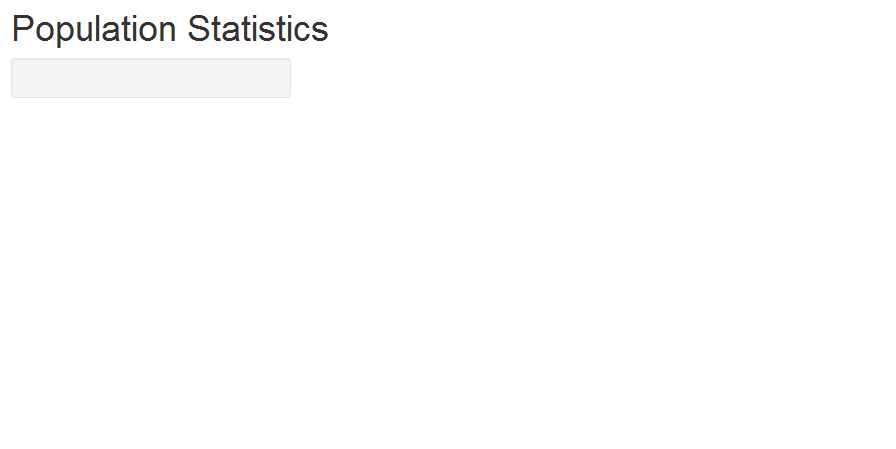
\includegraphics[width=0.5\textwidth]{pictures/shiny/blank.PNG} 
   \caption{Blank Shiny App}
   \label{fig:blank}
\end{figure}
To begin the model, we need to display the inputs of our program in the sidebar panel of the application.
Our program is taking age group as an input and displaying a plot showing the predicted populations of that age group in North Carolina over the next five years.
To do this, we will create a selectInput with all of the age groups as choices, like so:
\begin{lstlisting}[language = R]
sidebarPanel(
    selectInput(
        inputId = "age", 
        label = "Age:", 
        choices = c(
            "Total", "0-4 years", "5-9 years", 
            "10-14 years", "15-19 years", "20-24 years", 
            "25-29 years", "30-34 years", "35-39 years", 
            "40-44 years", "45-49 years", "50-54 years", 
            "55-59 years", "60-64 years", "65-69 years", 
            "70-74 years", "75-79 years", "80-84 years", 
            "85+ years")
    )
  )
\end{lstlisting}
The \texttt{inputId} is simply a name that we give to each input, so we can access them in the server function.
The label is the text that will appear on the application above the input box.

We also need to tell the application that our plot will be displayed in the main panel of the UI.
This involves creating a \texttt{plotOuput}, like so: 
\begin{lstlisting}[language = R]
 mainPanel(
    plotOutput(outputId = "myPlot")
 )
\end{lstlisting}
Just like in \texttt{selectInput}, we need to give the output an ID, so we can use that name to access it in the \texttt{server} function.
Once the model is run, the application should look like figure \ref{fig:drop}. 
\begin{figure}[htbp!]
   \centering
   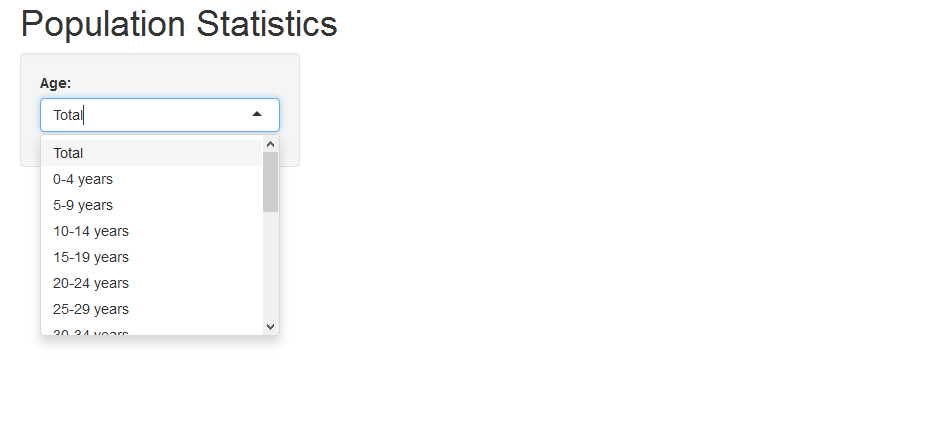
\includegraphics[width=0.5\textwidth]{pictures/shiny/dropdown.PNG} 
   \caption{Adding Inputs}
   \label{fig:drop}
\end{figure}
Next we need to define the server-side of the application which will accept inputs and compute outputs.
Our \texttt{server} function will contain the code necessary to do this.
We first tell the function that we are creating a plot as an output, and we can create the plot using the \texttt{renderPlot} command.
The command \texttt{renderPlot} is what makes the application react.
This means when a user changes the input, the output will instantly change.
This is what makes Shiny so interactive.

Within the renderPlot function we first select what data we will use and then plot that data using the ggplot function.
To select our data, create a variable called \texttt{dataInput}, and take a subset of the \texttt{.csv} file we imported into R.
We want to take only the data that the user specified, so instead of importing all the age group data, we only import the age group that the user selected.
We can access that specific age group using \texttt{input\$age}.
The \texttt{ggplot} function takes in various inputs, such as the data, the variables, and the title.
The \texttt{aes} function within \texttt{ggplot} indicates which axis is given to which variable, while the \texttt{geom\_point} function draws the points on the graph.
The \texttt{ggtitle} function creates a title over the plot.
The completed \texttt{server} function should look like this: 
\begin{lstlisting}[language = R]
server <- function(input, output) {
  output\$myPlot <- renderPlot({
    dataInput <- subset(popData, (Age==input\$age), select=c(Year, Population, State))
    
    ggplot(
        data = dataInput, 
        aes(x=Year, y=Population)
    ) + geom_point() + ggtitle("Population")
    
 })
  
}
\end{lstlisting}
Finally, run the entire code including the \texttt{shinyApp} command.
Your screen should look like the screen displayed in Figure \ref{fig:example}.
The application should have a working select box, a title, and a plot displaying the population data.
\begin{figure}[htbp!]
   \centering
   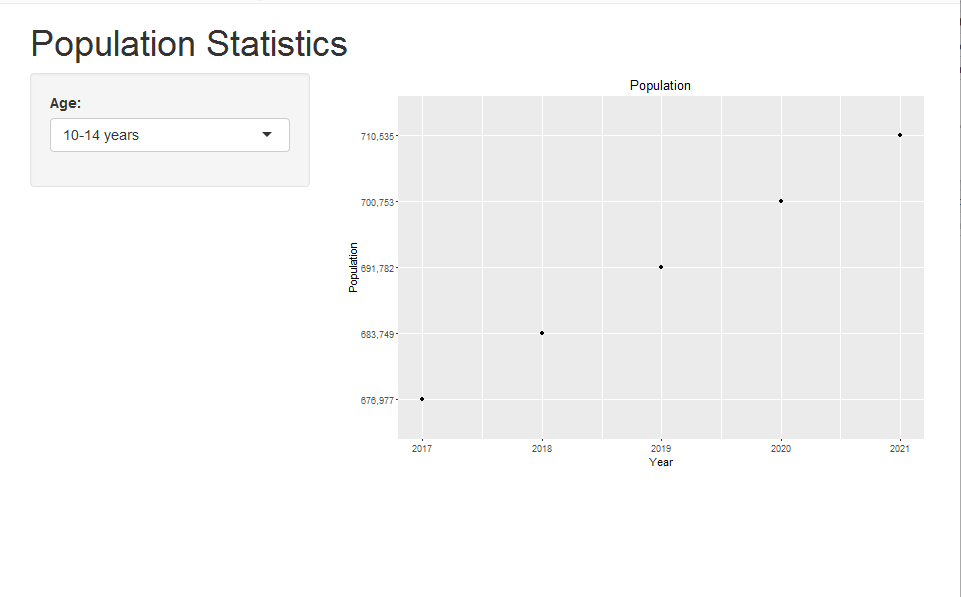
\includegraphics[width = .5\textwidth]{pictures/shiny/pop.PNG} 
   \caption{Final Model}
   \label{fig:example}
\end{figure}

\section{Deliverable}

You are expected to deliver properly formatted code written in the R language, using the Shiny package.
Additionally, you will need to provide screenshots of various input combinations to demonstrate that your application is fully functional.
This model will display Olympic swimming times over the modern Olympics.
The variables for this model include time, year, and medal.
The inputs are the event and gender of the swimmer.
The graph should display the medaling times for each event and gender for each year of the modern Olympics.
The data for this project is found within the \texttt{SwimmingExampleM} dataset provided. 
\subsection{Programming Hints}
In the deliverable you will need to be able to add color to the model.
It is quite simple.
In the previous section we explained that the \texttt{ggplot} command makes the actual plot.
In order to create color we just add \texttt{color = variablename}, inside the \texttt{aes()} function.

\begin{lstlisting}[language = R]
aes(x=Time, y=Year, color=Medal)
\end{lstlisting}
The final shiny app screen should look like figure \ref{fig:olympic}
\begin{figure}[htbp!]
   \centering
   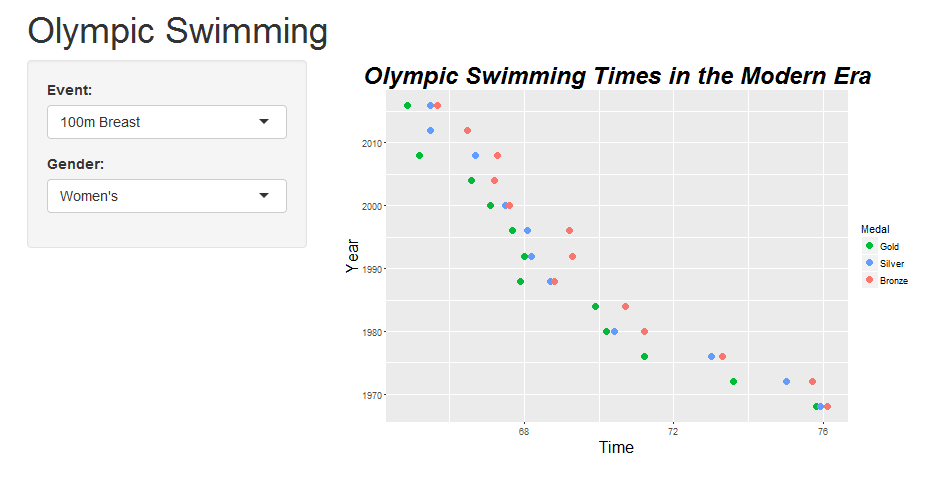
\includegraphics[width = .5\textwidth]{pictures/shiny/olympic.PNG} 
   \caption{Deliverable}
   \label{fig:olympic}
\end{figure}

\section{Teaching Code}
\begin{lstlisting}[language = R]
#Ishaan Rao
#September 1, 2016
#pop.R

#clean up and set the directory
rm(list=ls())
setwd("C:/Users/Ishaan/Documents/NCSSM 2015-2016")

#load libraries
library(ggplot2)
library(scales)
library(ggmap)
library(dplyr)
library(car)
library(gcookbook)
library(shiny)

#read data file
popData <- read.csv("Population.csv")

#setting the server, code instructing R what to do with inputs
#output\$my plot is what will be created when the app is run
#renderPlot allows Shiny to adjust when the user changes an option
#By defining the subset we indicate which inputs we want to be selected by the user
#select are the values in the dataset that are going to be plotted
#ggplot give direction to create plot, aes() defines the axes, ggtitle creates 
title and geom_point creates the scatter plot
server <- function(input, output) {
  output\$myPlot <- renderPlot({
    dataInput <- subset(popData, (Age==input\$age), select=c(Year, Population, State))
    
    ggplot(data = dataInput, aes(x=Year, y=Population)) 
    + geom_point() + ggtitle("Population")
    
  })
  
}
# Define UI for application that draws a scatterplot
#headerPanel creates the title
#sidebarPanel creates the user entered section
#selectInputs is where you insert the options that the user can select
#mainPanel outputs the app using all of the previous code we inputed
ui <- shinyUI(fluidPage(
  headerPanel("Population Statistics"),
  sidebarPanel(
    selectInput(
        inputId = "age", 
        label = "Age:", 
        choices = c(
            "Total", "0-4 years", "5-9 years", 
            "10-14 years", "15-19 years", "20-24 years", 
            "25-29 years", "30-34 years", "35-39 years", 
            "40-44 years", "45-49 years", "50-54 years", 
            "55-59 years", "60-64 years", "65-69 years", 
            "70-74 years", "75-79 years", "80-84 years", 
            "85+ years")
    )
  ),
  mainPanel(
    plotOutput(outputId = "myPlot")
  )
))
#this runs the Shiny App
shinyApp(ui = ui, server = server)

\end{lstlisting}

\section{Example Student Code}

\begin{lstlisting}[language = R]
#Ishaan Rao
#September 1, 2016
#olympic.R

#load libraries
library(ggplot2)
library(scales)
library(ggmap)
library(dplyr)
library(car)
library(gcookbook)
library(shiny)

rm(list=ls())
setwd("C:/Users/Ishaan/Documents/NCSSM 2015-2016")

swimData <- read.csv("SwimExampleM.csv")
#setting the server, code instructing R what to do with inputs
#output\$my plot is what will be created when the app is run
#renderPlot allows Shiny to adjust when the user changes an option
#By defining the subset we indicate which inputs we want to be selected by the user
#select are the values in the dataset that are going to be plotted
#ggplot give direction to create plot, aes() defines the axes, ggtitle creates 
title and geom_point creates the scatter plot
#scale_color_hue creates different colors for each of the three models\\
server <- function(input, output) {

  output\$myPlot <- renderPlot({
  
    dataInput <- subset(swimData,
             (Event==input\$event & Gender==input\$gender), 
                select=c(Time, Year, Medal, Name))
    
    ggplot(data = dataInput, aes(x=Time, y=Year, color=Medal)) + 
        geom_point(size=3) + 
        ggtitle("Olympic Swimming Times in the Modern Era") + 
        theme(
            plot.title = element_text(color="black", size=24, 
            family="Times", face="bold.italic"), axis.title = element_text(size=16)
        ) + 
        scale_color_hue(breaks=c("Gold","Silver","Bronze"))
  })
} 
# Define UI for application that draws a scatterplot
#headerPanel creates the title
#sidebarPanel creates the user entered section
#selectInputs is where you insert the options that the user can select
#In the model we have two different inputs one for event and one for gender, we 
create two different selectInput commands to account for the options
#mainPanel outputs the app using all of the previous code we inputted
ui <- shinyUI(fluidPage(
  headerPanel("Olympic Swimming"),
  sidebarPanel(
    selectInput(
        inputId = "event", 
        label = "Event:", 
        choices = c(
            "50m Free", "100m Free", "100m Back", "100m Breast", 
            "100m Butterfly", "200m Free", "200m Back", "200m Breast",
            "200m Butterfly", "200m IM", "400m IM"
        ), 
        selected = "50m Free"
    ),
    selectInput(
        inputId = "gender", 
        label = "Gender:", 
        choices = c("Men's", "Women's"),
        selected = "Women's"
    )
  ),
  mainPanel(
    plotOutput("myPlot")
  )
))
#runs application
shinyApp(ui = ui, server = server)
\end{lstlisting}


\section{Further Readings}
\begin{itemize}
\item For a full tutorial on creating a Shiny app, visit this tutorial on the Shiny website: \url{http://shiny.rstudio.com/tutorial/}.
\item To learn more advanced Shiny topics, functions, and capabilities visit: \url{http://shiny.rstudio.com/articles/}.
\item To see sample Shiny apps in action visit Shiny's gallery: \url{http://shiny.rstudio.com/gallery/}
\end{itemize}


\chapterimage{Pictures/ChapterHeadings/header_06.jpg}

\chapter{deSolve}
\section{Introduction to Computational Differential Solutions}

Many of the systems studied in life sciences, environmental sciences, and physical sciences can be modeled with differential equations.
Differential equations serve to model rates of change, which are often easier to measure than every interaction in the system.
A differential equation is an equation for a function that relates the values of the function to the values of its derivatives.
An ordinary differential equation (ODE) is a differential equation for a function of a single variable (such as $x(t)$), while a partial differential equation (PDE) is a differential equation for a function of several variables (such as $v(x,y,z,t)$).
An ODE contains ordinary derivatives and a PDE contains partial derivatives. Typically,PDE's are much harder to solve than ODE's \cite{chasnov}.

Initial Value Problems (IVPs) involve differential equations where certain initial values in the model are known.
The \texttt{deSolve} package uses computational means to analyze and compute the values of states in such models.
In a differential equation, the state is the variable that is varied with respect to the independent variable in the system.
Parameters, on the other hand, are values that signify some characteristic or attribute of the system.
For example, in the given system of equations:

\begin{equation*}
    \frac{dY}{dt}=aY
\end{equation*}

The state of the differential equation is $Y$.
The independent variable in this system is $t$.
Finally, $a$ is a parameter that can be varied to vary the solution.
In this lab, we will analyze systems of ordinary first-order differential equations, which relate the first derivative to states and parameters.

\subsection{Examples of Differential Equations}

The \textit{Malthusian law of population growth} is used to model the populations of certain kinds of organisms living in ideal environments for limited lengths of time $t$.
It gives the rate at which a population $p$ changes with respect to $t$.
The value of the constant $r$ depends on the organism.

\begin{gather*}
    \frac{dp}{dt}=rp
\end{gather*}

This \textit{second-order reaction rate} law gives the rate at which a single chemical species combines to produce a new species, such as methyl radicals combining in a gas to form ethane molecules.

\begin{gather*}
    \frac{dx}{dt}=k(A-x)^2
\end{gather*}

This equation models the motion of a damped mass-spring system subjected to a time-dependent force $F(t)$.

\begin{gather*}
    m\frac{d^2 x}{dt^2}+b\frac{dx}{dt}+kx=F(t)
\end{gather*}

\section{Installation}

To install the \texttt{deSolve} package in R, enter the following code into the command line.
Installation may produce warnings that are generally inconsequential to the overall usage of the package.
However, if the package does not install correctly, contact the package developers.

\begin{lstlisting}
 > install.packages(``deSolve'')
 > library(deSolve)
\end{lstlisting}

\section{Objectives of Case Study}

There are certain objectives that students should focus to accomplish while completing this activity. 

\begin{itemize}
\item Know what ordinary differential equations and partial differential equations are.
For the case studies that follow, it is inconsequential for students to understand the structure and function of ordinary differential equations.

\item Understand how initial value problems arise in ordinary differential equation systems in the natural sciences.
That is, use initial values found in nature and differential equation models to produce valid solutions.

\item Know how to set up a differential equation given a system and the relationship between rates.
This is important for modeling a given system.

\item Know how to use \texttt{deSolve} to computationally solve systems of ordinary first-order differential equations.
This R package allows for computational solutions that effectively model the changes in the dependent variables of the system.
\end{itemize}

\section{Case Study - Dampened Mass-Spring System}

As discussed in the examples section, a well-known second-order differential equation is used to analyze the motion of an oscillating mass-spring. 

\begin{figure}[H]
    \centering
    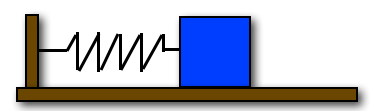
\includegraphics[width=15cm]{pictures/diffeq/mass-spring.jpeg}
    \caption{A mass-spring system}
\end{figure}

A mass-spring system is often called a harmonic oscillator.
In an idealized system where no heat loss occurs, the mass-spring oscillator will continue oscillating forever. 

The nature of a spring can be described using a single parameter, often noted as $k$.
The spring constant $k$ is used primarily in Hooke's Law, which relates the amount a spring stretches from rest, $x$, to the amount of force $F$ that is applied on the mass $m$.
Hooke's Law states that:

\begin{gather*}
    F=-kx
\end{gather*}

By Newton's Second Law, we also know that:

\begin{gather*}
    F=m\frac{d^2 x}{dt^2}
\end{gather*}

Therefore, we can create a second-order differential equation for the idealized mass-spring oscillator:

\begin{gather*}
    m\frac{d^2 x}{dt^2}=-kx\\
    \boxed{m\frac{d^2 x}{dt^2}+kx=0}
\end{gather*}

Unfortunately, due to the complexity of behaviors and solutions in second-order differential equations, it is computationally easier to create a system of differential equations $x_1', x_2', \hdots, x_n'$ that model the system.

We begin with a few basic states that will represent the differential equations in our system.

\begin{gather*}
    x_1 = x\\
    x_2 = \frac{dx}{dt}
\end{gather*}

We compute the derivatives of these states:

\begin{gather*}
    x_1' = x' = x_2\\
    x_2' = x''
\end{gather*}

By solving the second-order differential equation in terms of the second derivative $x''$:

\begin{gather*}
    m\frac{d^2 x}{dt^2}+kx=0\\
    mx''+kx=0\\
    x''=-\frac{k}{m}x=-\frac{k}{m}x_1
\end{gather*}

Therefore, the system of ordinary first-order differential equations that we are trying to solve is:

\begin{gather*}
    \frac{dx_1}{dt}=x_2\\
    \frac{dx_2}{dt}=-\frac{k}{m}x_1
\end{gather*}

\subsection{Computational Solutions}

We begin by setting up the environment to begin using the \texttt{deSolve} package. We import the library and clear the environment variables.

\begin{lstlisting}
# Author:       First Last
# Date:         Month Date Year
# Name:         DiffEq.R

# Import the library into R
library(deSolve)

# Clear variables from environment
rm(list = ls())
\end{lstlisting}

As stated in the introduction, we are solving an initial value problem.
In this case, we use arbitrary values for states and parameters.
We initialize $x_1=100$ to suggest that the spring is stretched 100 meters past it's rest phase.
Furthermore, $x_2=0$ to suggest that the motion begins from rest, when the rate of change is 0.

\begin{lstlisting}
# m is the mass of the object (1 kg)
# k is the spring constant (50 kg / s^2)
parameters <- c(m = 1, k = 50)

# X is the first differential equation (100 m)
# Y is the second differential equation (0 m/s)
state <- c(X = 100, Y = 0)
\end{lstlisting}

We can define a function that represents the system of differential equations we have defined.
Such a function will effectively relate the state and parameters to the derivatives in question. 

\begin{lstlisting}
# Function that defines the system
system <- function(t, state, parameters) {
    with(as.list(c(state, parameters)), {
        dX <- Y
        dY <- -1*(k/m)X
        
        list(c(dX, dY))
    })
}
\end{lstlisting}

We run the simulation over a certain time interval with discreet differences between every time value.
Finally, we run the \texttt{ode()} function to produce the discreet values.

\begin{lstlisting}
# The sequence of time run in the simulation
times <- seq(0, 10, by=0.01)

# Generate curves that are solutions to the system of differential equations
out <- ode(y=state, times=times,func=system, parms=parameters)
\end{lstlisting}

Running the command above will generate data that is stored in \texttt{out}.
We can plot this data out.
From our derivation, we know that the value of $x_1=x$.
Therefore, the solution to $x_1$ is equal to the solution of the second-order differential equation.
We also plot how the two variables, $x_1$ and $x_2$, vary in comparison to each other.
We plot the following:

\begin{lstlisting}
plot(out[,"time"], out[,"X"], xlab="time", ylab="displacement", pch=19)
plot(out[,"X"], out[,"Y"], xlab="displacement", ylab="velocity", pch=19)
\end{lstlisting}

\begin{figure}[H]
    \centering
    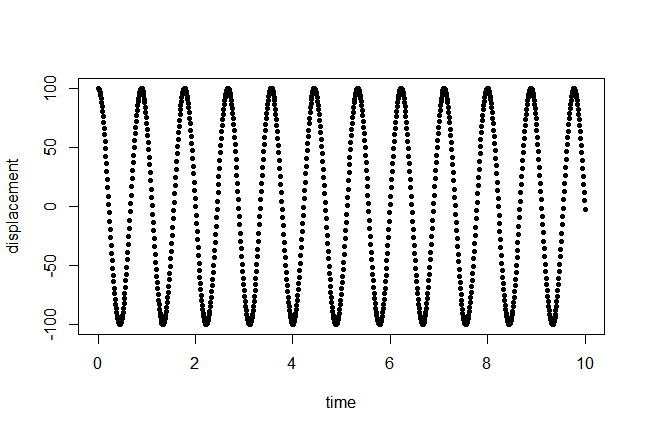
\includegraphics[width=12cm]{pictures/diffeq/plot1.png}
    \caption{The displacement of the spring over time}
\end{figure}

\begin{figure}[H]
    \centering
    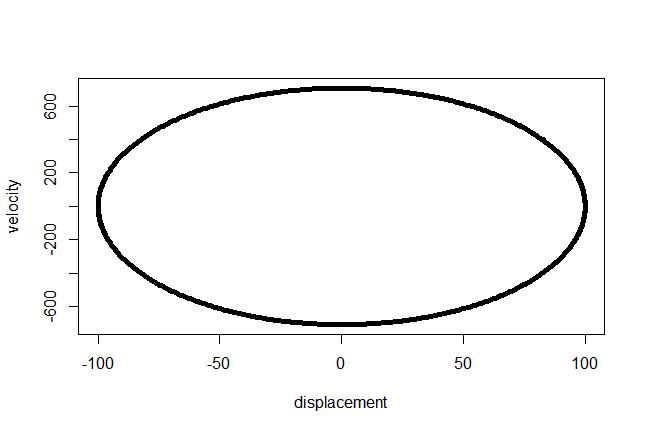
\includegraphics[width=12cm]{pictures/diffeq/plot2.png}
    \caption{The relationship between $x_1$ and $x_2$}
\end{figure}

\subsection{Improving the System}

However, this idealized system does not capture the motion of a spring that is dampened by other factors, such as heat loss by friction.
Such a system is known as a \textbf{Dampened Mass-Spring Oscillator}.
The spring looses momentum with relation to its velocity, which is the derivative of the position $x$.
Therefore, we can add a new parameter to the second-order differential equation, $b$, that accounts for the dampening of the motion of the spring.

\begin{gather*}
    m\frac{d^2 x}{dt^2}+b\frac{dx}{dt}+kx=0
\end{gather*}

Using the method described above to convert the second-order differential equation into a system of first-order differential equations, we get:

\begin{gather*}
\frac{dx_1}{dt}=x_2\\
\frac{dx_2}{dt}=-\frac{k}{m}x_1 - \frac{b}{m}x_2
\end{gather*}

We modify our systems function in R to account for the velocity-dependent dampening of the spring as follows:

\begin{lstlisting}
# m is the mass of the object (1 kg)
# b is the dampening of the object (0.25)
# k is the spring constant (50 kg / s^2)
parameters <- c(m = 1, b = 0.25, k = 50)

# Function that defines the system
system <- function(t, state, parameters) {
    with(as.list(c(state, parameters)), {
        dX <- Y
        dY <- -1*(k/m)X - (b/m)Y
    })
}
\end{lstlisting}

Running the simulation again, we get the following graphs.
Notice that the range of the motion of the spring-mass system continually decreases as time passes.
This accounts for much of the heat loss that a dampened spring experiences. 

\begin{figure}[H]
    \centering
    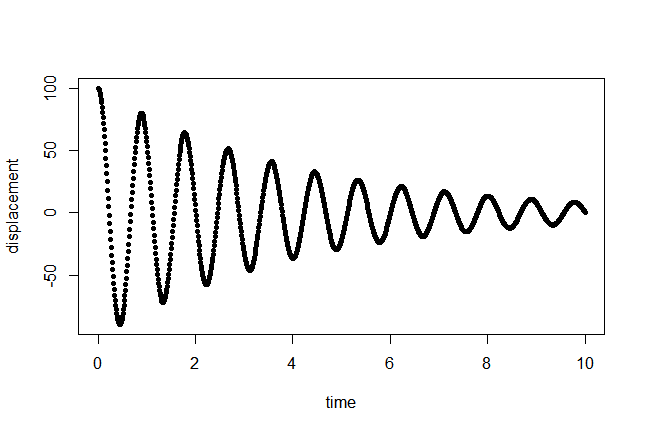
\includegraphics[width=12cm]{pictures/diffeq/plot3.png}
    \caption{The displacement of the spring over time}
\end{figure}

\begin{figure}[H]
    \centering
    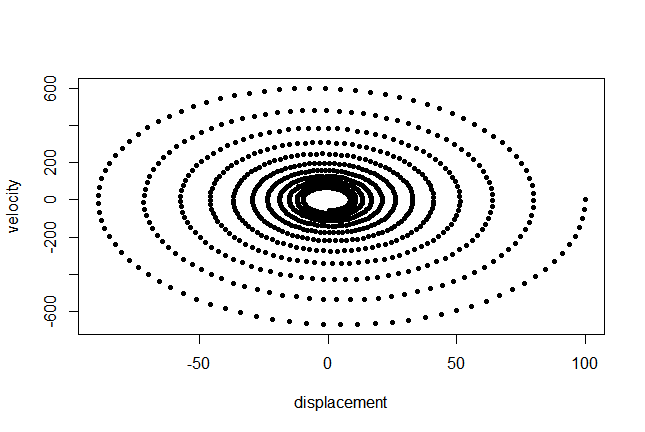
\includegraphics[width=12cm]{pictures/diffeq/plot4.png}
    \caption{The relationship between $x_1$ and $x_2$}
\end{figure}

\section{Student Assignment - Modelling of Genetic Processes}

Many of the genetic processes that are studied in the field of molecular biology can be modeled using systems of differential equations.
The student is tasked with understanding many of theses systems and modeling them.
It is important for us to go over the \textit{central dogma of molecular biology} before proceeding any further.

The three main components of this dogma are DNA, mRNA, and proteins.
Proteins are generally the effectors in our cells, responsible for life-critical tasks, enzymatic processes, and regulation.
Every protein has its own function and specificity.
Ribosomal subunits, responsible for synthesizing proteins, get instructions for synthesis from polymer strands made of nucleotides known as mRNA.
mRNA strands, in turn, are synthesized using instructions from another polymer known as DNA, which is the only heritable molecule present in the cell (as long as we ignore mitochondrial DNA that is passed down from a maternal lineage).
We will also quickly review the processes of transcription and translation in depth.
However, a strong foundation in biology is not necessary for modelling the problems that will follow. 

\begin{itemize}
    \item \textbf{Transcription: } Transcription is the process by which the information contained in a section of DNA (most often a gene) is transferred to a newly assembled piece of messenger RNA (mRNA).
    Transcription is triggered by the binding of RNA Polymerase to specific regions on the DNA called promoters, and is enabled/facilitated or impeded by a range fo promoter-specific proteins called transcription factors \cite{stan}.
    \item \textbf{Translation: } During translation, proteins are produced by ribosomes that bind to a specific site of the mRNA (the ribosome binding site - RBS) and then move along the mRNA chain converting triplets of bases or ``codons'' on the mRNA into the appropriate peptide chain of amino acids defining the desired protein.
    The mRNA is read by the ribosome as triplet of bases, usually beginning with an AUG, or an initiator methionine codon downstream of the ribosome binding site.
    Complexes of initiation factors and elongation factors bring aminoacylated transfer RNAs (tRNAs) into the riboosome-mRNA complex, matching the codon in the mRNA to the anti-codon in the tRNA, thereby adding the correct amino acid in the growing peptide sequence encoding the emerging protein.
    As the amino acids are linked together into the growing peptide chain, they begin folding into the correct conformation.
    This folding continues until the nascent polypeptide chain is released from the ribosome as a mature protein \cite{stan}.
\end{itemize}

\begin{figure}[H]
    \centering
    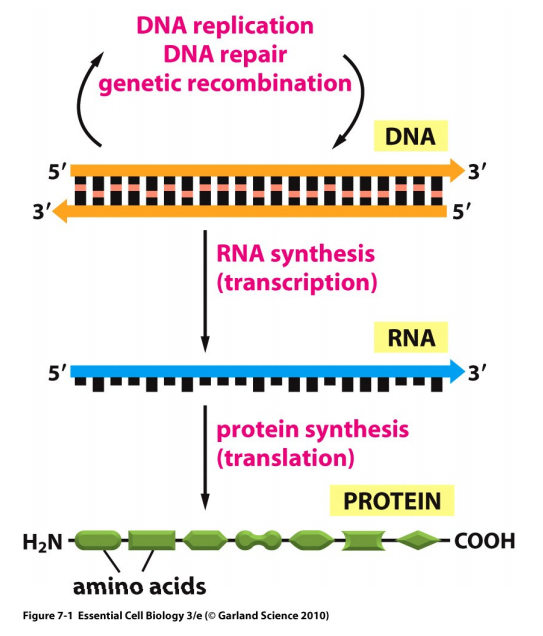
\includegraphics[width=10cm]{pictures/diffeq/img1.png}
    \caption{The Central Dogma of Molecular Biology}
\end{figure}

\subsection{Constitutive Gene Expression}

\textbf{Problem Statement: } Model the system of constitutive gene expression in terms of the central dogma of molecular biology, mRNA degradation, and protein degradation.

Constitutive gene expression is the process that occurs when a gene is always on.
That is, the gene is not regulated in any manner and simply follows the central dogma of biology.
In such a case, we have to consider a few rates that occur in the system. 

\begin{itemize}
    \item $\frac{dm}{dt}$ is the rate at which mRNA is synthesized from DNA.
    It will be one of the differential equations students will use in their system.
    \item $\frac{dp}{dt}$ is the rate at which the protein in question is synthesized from DNA.
    It will be the other differential equation students will consider in their system.
    \item $k_{m}$ is the constitutive transcription rate.
    It is considered to be constant, and it represents the number of mRNA molecules produced per gene, per unit of time.
    We assume that there is only one copy of the gene in the cell.
    In the case of bacterial cells, where plasmid-located genes occur in multiple copies in different plasmids, we would multiply the rate $k_1$ by the number of copies $N$ in the cell to obtain a proper rate.
    \item $k_{p}$ is the translation rate.
    It is considered to be constant, and it represents the number or protein molecules produced per mRNA molecule, per unit of time.
    \item $d_{m}$ is the mRNA degradation rate, measured as the frequency at which mRNA molecules degrade.
    \item $d_{p}$ is the protein degradation rate, measured as the frequency at which protein molecules degrade.
\end{itemize}

\noindent \textbf{Sample Student Solution}

The student should be capable of modeling the system using the rates provided above.
The system we are considering should account for transcription, translation, and the degradation of components in the process.

\begin{figure}[H]
    \centering
    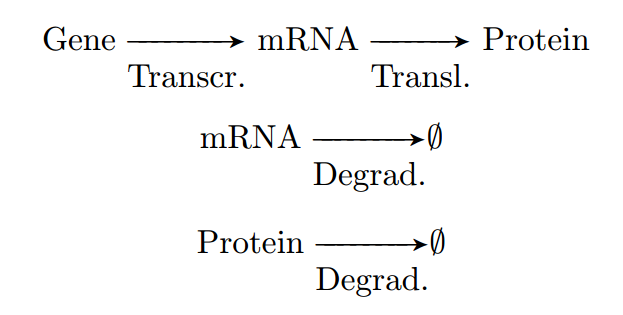
\includegraphics[width=8cm]{pictures/diffeq/img2.png}
    \caption{The constitutive gene expression system}
\end{figure}

The rate at which mRNA is transcribed is equal to the rate provided to us, $k_{m}$.
Furthermore, we account for the rate of degradation by multiplying the frequency rate $d_{m}$ by the number of mRNA molecules in the system.
The rate at which protein molecules are translated is equal to the rate $k_{p}$.
Similar to the mRNA system, the degradation occurs as a product of $d_{p}$ and the amount of protein produced. 

\begin{gather*}
    \frac{dm}{dt}=k_{m}-d_{m}m\\
    \frac{dp}{dt}=k_{p}m-d_{p}p
\end{gather*}

The student simply has to change certain aspects of the program written by the instructor.
In this case, the student must define a new set of states, parameters, and a new system function.

\begin{lstlisting}
library(deSolve)

parameters <- c(km = 10, kp = 5, dm = 1, dp = 3)
state <- c(M = 0, P = 0)

system <- function(t, state, parameters) {
    with(as.list(c(state, parameters)), {
        dM <- km - dm*M
        dP <- dp*M - dp*P
        
        list(c(dM, dP))
    })
}

times <- seq(0, 10, by=0.01)

out <- ode(y = state, times = times, func = system, parms = parameters)

# Plotting Functions
xaxis.range <- range(times)
yaxis.range <- range(min(range(out[,"M"]), range(out[,"P"])), max(range(out[,"M"]), range(out[,"P"])))
plot(out[,"time"], out[,"M"], xlim=xaxis.range, ylim=yaxis.range, col="red", xlab="Time", ylab="Concentration", main="System", pch=19)
points(out[,"time"], out[,"P"], col="blue", pch=19)
legend("bottomright", c("mRNA", "Protein"), pch=c(19, 19), col=c("red", "blue"))
\end{lstlisting}

\begin{figure}[H]
    \centering
    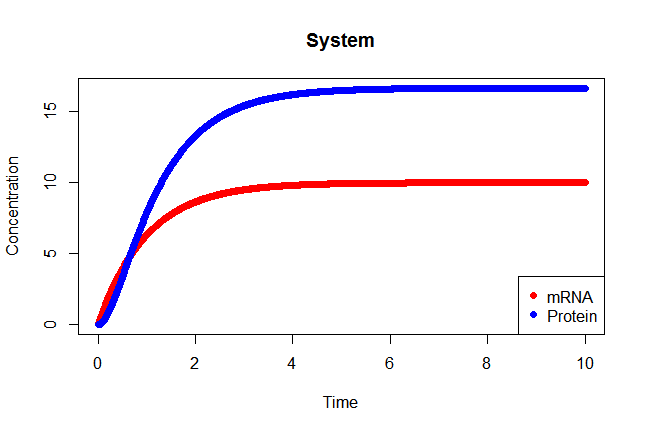
\includegraphics[width=.5\textwidth]{pictures/diffeq/plot5.png}
    \caption{Constitutive gene expression concentrations in the system}
\end{figure}

We see that the concentration of proteins and mRNA in the system reaches a steady state with the initial values supplied.
It is important for the student to understand that varying the parameters can change the solution to the system.
For example, if the rate of degradation of a protein is much larger than the rate at which it is produced, we expect to see no overall protein production.
Therefore, it is just as important to choose appropriate initial values as it is to produce a sound differential model.
Although arbitrary values are chosen for these samples, students are encouraged to read literature in their field of research or study to find common values for such problems.
For instance, the average half life of mRNA in the model system \textit{E.coli} is around 5 minutes.
Such information is inconsequential to producing an appropriate model.

\subsection{Gene Transcription Regulation}

Interestingly, most genes that are known today do not follow the constitutive gene expression model.
The constant production of proteins can be unnecessary, if not harmful, to  the proper function of the organism.
Therefore, multiple layers of regulation occur to ensure that the gene produces proteins at the correct time and the proper rate.
There are two major arguments for the necessity of gene regulation in cellular and molecular biology.
Firstly, all cells carry the same DNA (and therefore, the same heritable information) but have different developmental stages and functions.
Secondly, cells are subject to many environmental perturbations, which can only be dealt with by regulation.

Proteins known as transcription factors are generally responsible for the regulation of genes.
Transcription factors attach to a region upstream of the gene known as the promoter.
The transcription factor can either be an activator (promotes the transcription of the gene) or a repressor (inhibits the transcription of the gene). 

\begin{figure}[H]
    \centering
    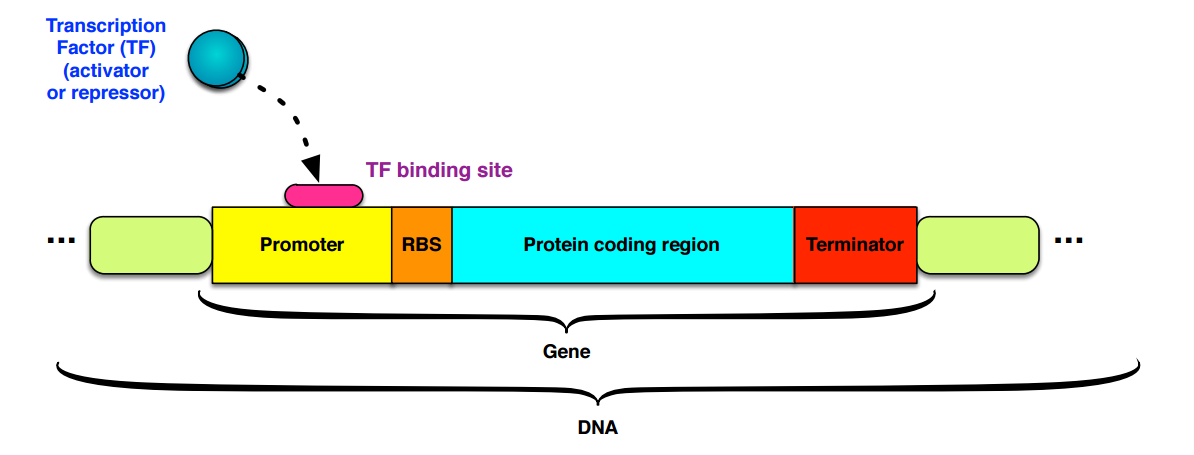
\includegraphics[width=.5\textwidth]{pictures/diffeq/img3.png}
    \caption{Action of regulative transcription factors on protein-encodoing DNA regions}
\end{figure}

\subsubsection{Activators and Repressors}

\textbf{Problem Statement: } Model the case of a gene whose transcription is activated by the binding of an activator/repressor to its transcription factor binding site.\\

A gene begins transcription once an activator binds to its corresponding transcription factor binding site.
Once activated, the gene goes through the same process that it would during constitutive gene expression.
These processes are inhibited once a repressor binds to the transcription factor binding site.
This process as a whole is the basis of gene regulation.
Because of the fact that, save for the introduction of activators and repressors, the process that the gene undergoes is identical to constitutive gene expression, many of the rates from the constitutive gene expression section are the same in this case.
These include $\frac{dm}{dt}$, $\frac{dp}{dt}$, $k_{m}$, $k_{p}$, $d_{m}$, and $d_{p}$.
With the introduction of a new parameter (an activator or a repressor), there are subsequently new variables added to this model.
The repressor and activator cannot occur at the same time, as the gene can only be activated or inhibited at a certain point in time.
These are as follows.

\begin{itemize}
    \item $A$ represents the activator.
    \item $R$ represents the repressor.
    \item $K$ represents the activation or repression coefficient.
    \item $n$ represents the Hill coefficient, or the number of activators/repressors that need to cooperatively bind to the promoter (transcription factor binding site) in order for gene expression to be activated/inhibited.
\end{itemize}

\noindent \textbf{Sample Student Solution} 

The student should be capable of modeling the system using the rates provided in the constitutive gene expression section, as well as using the new variables provided above.
The system we are considering should account for transcription, translation, and the degradation of components in the process.
\begin{figure}[H]
    \centering
    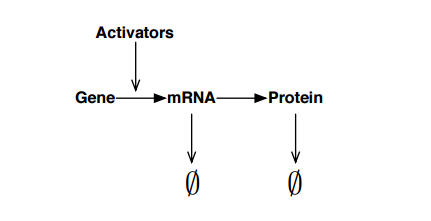
\includegraphics[width=.5\textwidth]{pictures/diffeq/activator.png}
    \caption{The activation and subsequent activities of a gene}
\end{figure}
\begin{figure}[H]
    \centering
    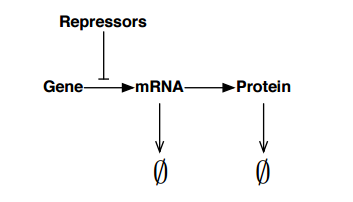
\includegraphics[width=.5\textwidth]{pictures/diffeq/Repressors.PNG}
    \caption{The inhibition and subsequent activities of a gene}
\end{figure}

The differential equations used in this model are almost identical to the differential equations used in previous models (the constitutive gene expression model).
The only difference is the introduction of the activator/repressor and its coefficients, which is then multiplied by $k_{m}$. 

These are the new differential equations with the introduction of the activator:
\begin{gather*}
    \frac{dm}{dt}=k_{m}\frac{A^{n}}{K^{n}+A^{n}}-d_{m}m\\
    \frac{dp}{dt}=k_{p}m-d_{p}p
\end{gather*}

These are the new differential equations with the introduction of the repressor:
\begin{gather*}
    \frac{dm}{dt}=k_{m}\frac{K^{n}}{K^{n}+R^{n}}-d_{m}m\\
    \frac{dp}{dt}=k_{p}m-d_{p}p
\end{gather*}

As with other cases, the student must define a new set of parameters and system functions in the code.
Most of the code remains the same.
The following shows the code when using the activator differential equations.

\begin{lstlisting}
library(deSolve)

parameters <- c(km = 10, kp = 5, dm = 4, dp =  4, A = 0.25, K = 0.01, n = 4)
state <- c(M = 0, P = 0)

system <- function(t, state, parameters) {
    with(as.list(c(state, parameters)), {
        dM <- km*(A^n/(K^n+A^n)) - dm*M
        dP <- dp*M - dp*P
        
        list(c(dM, dP))
    })
}
\end{lstlisting}

\begin{figure}[H]
    \centering
    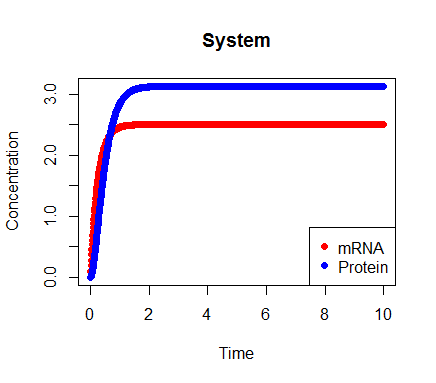
\includegraphics[width=.5\textwidth]{pictures/diffeq/activatorplot.png}
    \caption{Gene expression in a system containing activators}
\end{figure}

\subsection{Regulation}

Unfortunately, by simply solving each system individually, it is hard to tell how activation and inhibition affect gene expression models.
With the ability to model constitutive gene expression along with activation and regulation, we can compare models where activation and regulation does occur.
Using the following values, we can create three concurrent systems and compare them:

\begin{lstlisting}
# New parameters in the code
parameters <- c(km = 0.346, kp = 6.931, dm = 0.138, dp = 0.017, A = 200, R = 200, K = 100, n = 2)
state <- c(M = 0, P = 0)

# Constitutive Gene Expression Model
system.const <- function(t, state, parameters) {
    with(as.list(c(state, parameters)), {
        dM <- km - dm*M
        dP <- kp*M - kp*P
        
        list(c(dM, dP))
    }
}

# Activation in Gene Expression
system.act <- function(t, state, parameters) {
    with(as.list(c(state, parameters)), {
        dM <- dm*(A^n / (K^n + A^n)) - dm*M
        dP <- kp*M - dp*P
        
        list(c(dM, dP))
    })
}

# Inhibition in Gene Expression
system.rep <- function(t, state, parameters) {
    with(as.list(c(state, parameters)), {
        dM <- kM*(K^n / (K^n + R^n)) - dm*M
        dP <- kp*M - dp*P
        
        list(c(dM, dP))
    })
}

# Independent variable
times <- seq(0, 400, by=1)

# Computing the solution to all three models
out.const <- ode(y = state, times = times, func = system.const, parms = parameters)
out.act <- ode(y = state, times = times, func = system.act, parms = parameters)
out.rep <- ode(y = state, times = times, func = system.rep, parms = parameters)

# Plotting functions
plot(out.const[,"time"], out.const[,"P"], col="red", xlab="Time", ylab="Concentration", main="System", pch=19)
points(out.act[,"time"], out.act[,"P"], col="green", pch=19)
points(out.rep[,"time"], out.rep[,"P"], col="yellow", pch=19)
legend("bottomright", c("Protein CONST", "Protein ACT", "Protein REP"), pch=c(19, 19, 19), col=c("red", "green", "yellow"))
\end{lstlisting}

The code will produce the following graphics.
Notice that the constitutive protein expression runs unaffected.
The activation gene expression curve takes longer to achieve expression because it takes time for activators to act as transcription factors before transcription can take place.
Furthermore, the repressed curve is much lower than both, as is expected from such systems.

\begin{figure}[H]
    \centering
    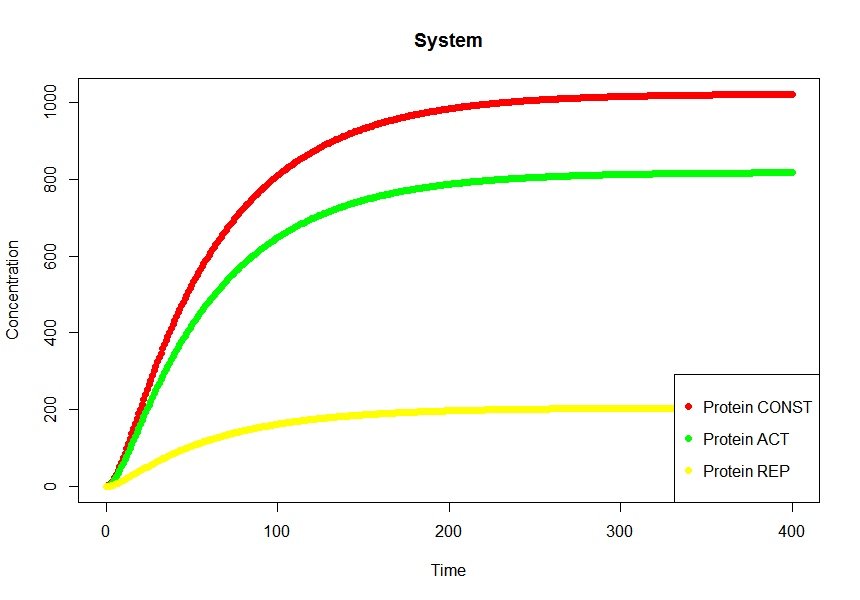
\includegraphics[width=.5\textwidth]{pictures/diffeq/plot6.png}
    \caption{Comparing constitutive, activation, and inhibition in gene expression.}
\end{figure}

\section{Conclusion}

Differential equations are used in a variety of different areas to model a wide range of functions, such as the rate that a protein is transcribed or the rate that a population grows.
The main function of a differential equation is to model a rate of change.
Some of these equations are easily solved by hand, whereas others are more complicated;
the \texttt{deSolve} package in R serves to solve and graph a system of differential equation once certain parameters and initial values are entered.
Through learning and using \texttt{deSolve}, it is possible to easily solve a system of complex differential equations, as well as view the results graphically and be able to change parameters and values as needed.
This streamlines a process of solving equations that occur within all types of science, math, and other processes.

\section{Acknowledgements}

We would like to thank the creators of the \texttt{deSolve} package, Karline Soetaert, Thomas Petzoldt, and R.
Woodrow Setzer of the Royal Netherlands Institute of Sea Research.
We would also like to thank Mr. Robert Gotwals and the North Carolina School of Science and Mathematics (NCSSM).

\begin{thebibliography}{3}
    \bibitem{soetaert}
        Karline Soetaert, Thomas Petzoldt, and R. Woodrow Setzer. ``Package deSolve: Initial Value Differential Equations in R.'' Royal Netherlands Institute of Sea Research (NIOZ), Yerseke, The Netherlands; Technische Universit{\"a}t, Dresden, Germany; National Center for Computational Toxicology, US Environmental Protection Agency, 2016 (\url{https://cran.r-project.org/web/packages/deSolve/vignettes/deSolve.pdf})
    \bibitem{chasnov}
        Jeffrey R. Chasnov. ``Introduction to Differential Equations.'' Hong Kong University of Science and Technology, 2016 (\url{https://www.math.ust.hk/~machas/differential-equations.pdf})
    \bibitem{stan}
        Dr. Guy-Bart Stan. ``Modelling in Biology,'' Department of Bioengineering, Imperial College of London, 2010 (\url{http://www.bg.ic.ac.uk/research/g.stan/2010_Course_MiB_article.pdf})
\end{thebibliography}


\chapterimage{Pictures/ChapterHeadings/header_07.jpg}

\chapter{Clustering}
\nomenclature{Glossary term:}{Definition}

Often, we are not only interested in specific data points, but also in the relationships between those data points.
Cluster analysis refers to the grouping of data points into \emph{clusters} based on similar characteristics.
R has variety of libraries that support cluster analysis.
We will use \texttt{cluster.datasets} for this lesson, in which we will analyze clustering in data about crime rates in US cities. \cite{Novomestky}
\medskip

Here are some typical commands used in cluster analysis:

\begin{enumerate}
\item \texttt{scale}
\item \texttt{k.means.fit}
\item \texttt{attributes}
\item \texttt{wssplot}
\item \texttt{clusplot}
\item \texttt{dist}
\item \texttt{hclust}
\item \texttt{groups}
\item \texttt{rect.hclust}
\item \texttt{table}

\end{enumerate}


For this study, you will learn a basic framework for cluster analysis using two different methods, K-means and hierarchical clustering.
Each method produces a different type of cluster graph of the same data. 

\begin{itemize}

\item Your first task is to graph a set of data using the K-means clustering method.

\item Your second task is to graph a set of data using the hierarchical clustering method. 
 
\end{itemize}

\section{Building the Model}

You should begin by copying and pasting the teaching code into RStudio.
This will serve as a foundation upon which to build your code.
We have included comments to guide you as you complete the code by adding commands.
When you successfully complete the code, it should output two graphics, shown in figures \ref{fig:Kmeans} and \ref{fig:Tree}.

\subsection{Programming Hints}

\begin{enumerate}
 
\item Different datasets will often require different clustering methods.
Therefore, not all clustering methods will work (or at least, work well) for every dataset!
Be prepared to use a variety of clustering methods in the future.
\item When installing packages, install them in the ``console'' window of RStudio.
\item If a piece of code is indented in the teaching or student code, it must also be indented in the code that you write.
This is important!
 
\end{enumerate}

\section{Deliverable}

The final product that you create should consist of one K-means cluster graph composed of groups of data points embedded in ovals and one hierarchical tree plot. 

\section{Teaching Code}

\begin{lstlisting}
    
# Your Name
# Date
# Script name: dataset.R
# Objective of script
#
# set working directory where results will be saved
setwd("file location")
#
# install the necessary package and datasets, then read in library
install.packages("data package") 
# this particular step should be completed in the console window
library(data package)
data(dataset, package = 'data package') 
# "dataset" is the name that you choose to call your specific dataset 
head(dataset)
#
# now we will begin to complete the first objective
#
# begin by standardizing the variables
dataset <- scale(original.dataset.name[-1])
#
# this next piece of code is the K-means function, where the number
# # symbol denotes the number of cluster groups
k.means.fit <- kmeans(dataset, #)
#
# this code segment includes all of the outputs of the k.means.fit function
attributes((k.means.fit))
#
# this next piece of code denotes the centroids
k.means.fit$centers # a nice table should result
#
# this piece of code shows the clusters
k.means.fit$cluster
#
# this code string denotes the size of the clusters
k.means.fit$size
#
# now we will begin to complete the first objective
#
# load the cluster library
library(cluster)
#
# this next section of code creates the a cluster graph using the K-means method
clusplot(dataset, k.means.fit$cluster, main = "Name of Cluster Graph", color = TRUE, 
shade = TRUE, labels = 2, lines = 0) # look at those nice colorful ovals!
#
# this next line creates a confusion matrix which evaluates the performance of the clustering
table(dataset[,1],k.means.fit$cluster)
#
# Okay, now that you've mastered k-means clustering, 
# let's move on to hierarchical clustering
# 
# this code segments defines the distance "d", which in 
# this case is Euclidean, for the clustering algorithm 
d <- dist(us.crime, method = "euclidean")
#
H.fit <- hclust(d, method = "ward.D")
#
# this displays the dendrogram
plot(H.fit)
#
# this separates the diagram into 4 groups...
groups <- cutree(H.fit, k=4)
#
# ... while this piece of code creates a red border around those same groups
rect.hclust(H.fit, k=4, border = "blue")
#
# lastly, another confusion matrix is used to evaluate the clustering
table(us.crime[,1],groups)
#
# end code

\end{lstlisting}

\section{Example Student Code}

\begin{lstlisting}

# Katherine L. Bennett
# September 1, 2016
# Script name: crime.R
# The purpose of this script is to analyse a sample of U.S. city crime 
# using two cluster analysis methods: K-means and Hierarchical
#
setwd("/Users/Katherine/Desktop/RFiles")
#
library(cluster.datasets)
data(us.crime, package = 'cluster.datasets')
head(us.crime)
#
us.crime <- scale(sample.us.city.crime.1970[-1])
#
k.means.fit <- kmeans(us.crime, 4)
#
attributes((k.means.fit))
k.means.fit$centers
k.means.fit$cluster
k.means.fit$size
#
library(cluster)
#
# the following two lines should be one line in your code 
# we have separated them in this guide for the reader's convenience
#
clusplot(us.crime, k.means.fit$cluster, main = "U.S. City Crime Cluster Representation", color = TRUE, 
shade = TRUE, labels = 2, lines = 0)
#
table(us.crime[,1],k.means.fit$cluster)
#
# hierarchical cluster method
#
d <- dist(us.crime, method = "euclidean")
H.fit <- hclust(d, method = "ward.D")
plot(H.fit)
groups <- cutree(H.fit, k=4)
rect.hclust(H.fit, k=4, border = "blue")
table(us.crime[,1],groups)
#
# end code

\end{lstlisting}

\global\csname @topnum\endcsname 0

\begin{figure}[htbp!]
    \centering
    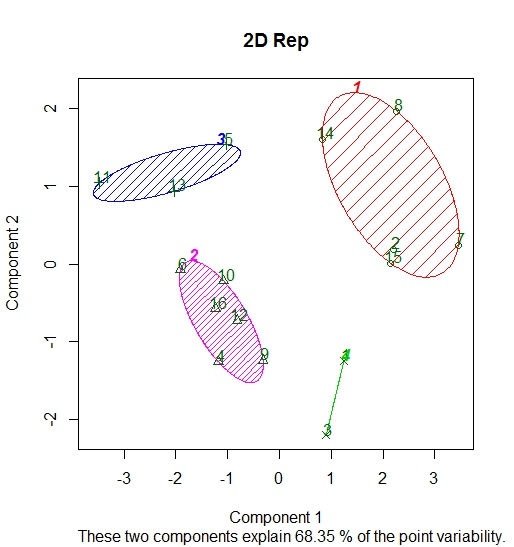
\includegraphics[width = .5\textwidth]{pictures/clustering/Kmeans.jpeg}
    \caption{K-means Clustering Method Result}
    \label{fig:Kmeans}
\end{figure}

\begin{figure}[htbp!]
    \centering
    \caption{Hierarchical Clustering Method Result}
    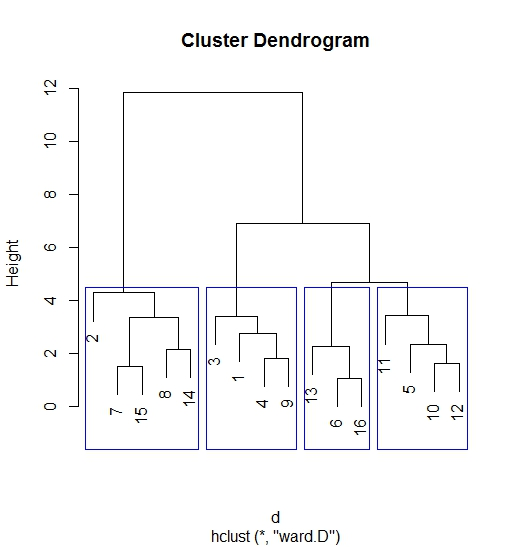
\includegraphics[width=0.5\textwidth]{pictures/clustering/Tree.jpeg}
    \label{fig:Tree}
\end{figure}

\section{Further Readings}

There are a wide variety of sources available that cover cluster analysis.
We recommend chapter 8 of \emph{Introduction to Data Mining} by Tan, Steinbach, and Kumar (2006).
A link to the chapter is provided below:

\url{https://www-users.cs.umn.edu/~kumar/dmbook/ch8.pdf}

\printnomenclature


\chapterimage{Pictures/ChapterHeadings/header_08.jpg}

\chapter{Microseq}
\section{Introductory Reading}

\nomenclature{Glossary term:}{Definition}

The conversion of working DNA to proteins is one of the most important processes in biology. After DNA undergoes transcription and becomes an mRNA sequence, it can be turned into a string of amino acids via sequences known as codons. Each codon consists of a combination of three nucleotides, and there are twenty amino acids that match with these combinations.

DNA and all DNA processes are integral to scientists' understanding of biology. Studying this molecule is a fascinating and essential task, but because of the large quantities of data that genetics studies can obtain, manually analyzing a sequence can prove to be insignificant. Bioinformatics is a relatively recent field that combines computational science, statistics, engineering, and biology in order to interpret this type of data. Being able to use technology to aid in the analysis of different sequences can greatly lessen the tediousness of translating sequences and manually visualizing data. It also eliminates the possibility of human error, and allows genetics research to move much faster.

For example, existing algorithms, such as JASPAR and STARR-seq, are databases or functional tools that allow bioinformaticians to analyze sequence data. These programs can do things such as identify even remotely homologous sequences from a DNA multiple sequence alignment, or identify \textit{cis-}regulatory regions throughout the genome. \cite{jaspar} The focus of this case study are R packages known as Biostrings and microseq, which, in conjuction, allow for sequence data analysis. 

\section{Objectives of the Case Study}

The objective of this study is to use the Biostrings and microseq packages in conjunction to translate a plain sequence format of DNA.

\subsection{Objective 1}

Translation of DNA to RNA is a vital biological process, and using the Biostrings and microseq functions will allow for a significantly streamlined process that will aid projects or studies in need of translated DNA. The objective is to obtqain an amino acid sequence translated automatically from the given DNA sequence.


\section{Building the Model}

Tips for building the model are located in the comment sections of the code.

If the code is written properly, the output should be a list with the frequencies of each amino acid in the DNA sequence. The output should look similar to figure \ref{fig:model}.

\begin{figure}[htbp!] %  the "H" means put it where you put this code....but that doesn't always work!
   \centering
   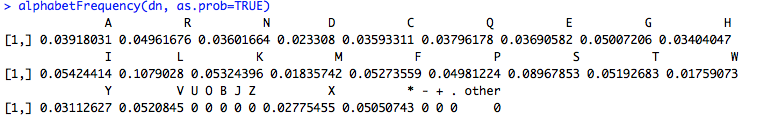
\includegraphics[width = \textwidth]{pictures/microseq/screenshot.png} 
   \caption{Frequency of amino acids}
   \label{fig:model}
\end{figure}

\section{Deliverable}

The student should submit a list containing the frequencies of each amino acid in the sequence analyzed. This list can be compared to the instructor's frequencies list to check for accuracy.

\section{Teaching Code}

You should also put any notes, teaching suggestions, etc. in this space!


\begin{lstlisting}
# Name
# Date
# Name of script
# Objective of script

# clean up and set working directory
rm(list=ls()) 
setwd()

### download data set from
ftp://ftp.ensembl.org/pub/release-85/fasta/mus_musculus/dna/

### install Biostrings from
https://bioconductor.org/packages/release/bioc/html/Biostrings.html
### then install microseq

#load  microseq and Biostrings library
library()
library()

# view accepted IUPAC DNA letters
# these are the values that the functions will accept and put out
DNA_BASES
DNA_ALPHABET

# obtain plain sequence format from .txt file on desktop or source
# turn fasta into string
d <- readDNAStringSet("data set")
# translate object to amino acid sequence
dn <- translate(data set, genetic.code=GENETIC_CODE, if.fuzzy.codon = "solve") 
#"solve" allows unidentifiable codons to be represented as *

#characteristics of DNA strings
d
summary(data set)
dn
summary(translated data set)

#frequency of each letter or present symbol
alphabetFrequency(translated data set)

#frequency values
alphabetFrequency(translated data set, as.prob=TRUE)

### EXTRA CREDIT!
letterFrequency(translated data set, "A", as.prob=TRUE)
letterFrequency(data set[[1]], letters="ACGT", OR=0)

# What do these two functions show? 
#show frequency of base "A" in translated data set, and quantity of "ACGT" in
original data set
\end{lstlisting}

\section{Example Student Code}

\begin{lstlisting}
# Christa Parrish
# September 8, 2016
# translate.R
# this script translates DNA sequence to Amino Acid sequence and observes frequencies 
of letters

# clean up and set working directory
rm(list=ls())
setwd("~/Desktop/R")

### download data set from ftp://ftp.ensembl.org/pub/release-85/fasta/mus_musculus/dna/

#load  microseq and Biostrings library
library(microseq)
library(Biostrings)

#view accepted IUPAC DNA letters
DNA_BASES
DNA_ALPHABET

# obtain plain sequence format from .txt file on desktop or source, whichever works
# turn fasta into object
d <- readDNAStringSet("MusMusculus.fa")
# translate object
dn <- translate(d, genetic.code=GENETIC_CODE, if.fuzzy.codon = "solve") 
#"solve" allows unidentifiable codons to be represented as *

#characteristics of DNA strings
d
summary(d)
dn
summary(dn)

#frequency of each letter or present symbol
alphabetFrequency(dn)

#frequency values
alphabetFrequency(dn, as.prob=TRUE)

### EXTRA CREDIT!
letterFrequency(dn, "A", as.prob=TRUE)
letterFrequency(d[[1]], letters="ACGT", OR=0)

# What do these two functions show?
\end{lstlisting}


\section{Further Readings}

By looking at the package manual online, students can read about the other functions of the microseq and Biostrings packages.

\printnomenclature


\chapterimage{Pictures/ChapterHeadings/header_09.jpg}

\chapter{Biodiversity}
\section{Introduction to Biodiversity}

The 21st century marks the era of big data.
This increase of data has effected all spheres of science, especially the study of biodiversity''
Biodiversity data covers an increasingly wide range of areas including bio-geography, ecology, invasive species biology, and climate change.
The information collected in biodiversity informatics projects has been used for studies relating to food security, control of disease vectors, and marine productivity \cite{Barve}.  
\begin{figure}[htbp!] 
   \centering
   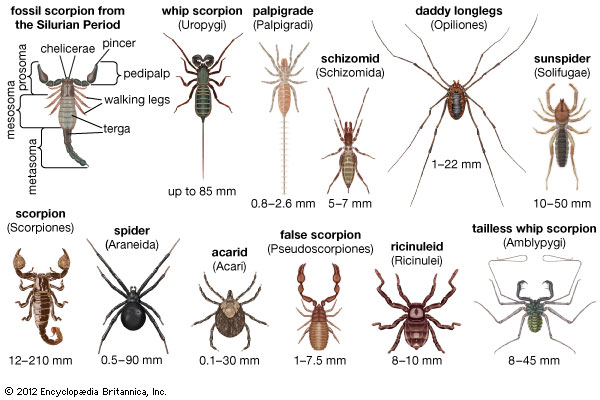
\includegraphics[width=0.5\textwidth]{pictures/biodiversity/spiders.jpg} 
   \caption{Example of biodiversity in arachnids}
   \label{fig:arachnids}
\end{figure}

Primary biodiversity data is one of the most important biodiversity statistics; it documents a species' occurrences in time and space.
Associated metadata, or data that describes statistics given in another set, may include information about who identified and recorded the species, who verified the identification, climatic parameters, micro-habitat information, number of individuals, sex, size, etc \cite{Barve}.
When these two types of data are formatted in universally accepted formats, published openly and integrated with other such data streams, they are known ``Digitally Accessible Knowledge'' or DAK.

There are many sources of biodiversity data including: directed surveys, broad-scale surveys, and biological collections. 

\subsection{Direct Surveys}

Directed surveys are often used where prior knowledge of a given system or biological mechanism exists.
Surveys for this type of experiment are designed to control for known sources of variation\cite {GBIFbirds}.
Direct surveys aim to establish a casual relationship between some experimental treatment and its effect and are widely accepted in the scientific community.
Regardless, the data collected in this type of survey is extremely expensive.
Additionally, the data is aggregated by many researchers working independently in small areas over small time scales, which creates a network of heterogeneous data repositories with little opportunity for integration and eventual data degradation.

\subsection{Broad  Surveys}

Broad-scale surveys involve over ten million observations annually.
This data is used to generate probabilistic estimates of species occurrence, which can then be used to determine general patterns over broad geographic regions and time scales \cite {GBIFbirds}.
Data for broad surveys can be collected by anyone, ranging from trained observers to interested citizens.
As a result, these surveys are relatively inexpensive to operate; however, the regulations behind these surveys are more relaxed, resulting in more potential for bias.
Nonetheless, these studies provide the bulk of non-specimen observational data available via the Internet \cite {SP}.

\subsection{Biological Collections}

Biological collections are data sets of specimens.
This type of data is primarily assembled to document the phenotypes and genotypes of the biotas worldwide \cite{Barve}.
Biological collections are typically considered as ``high-quality, low-volume'' sources of data on biological diversity \cite{Barve}.

Given all the different ways to collect data, each with their own pros and cons, it is important for researchers utilizing biodiversity data to determine the completeness and accuracy of their data sets.
Data visualization is one technique to observe patterns within very large data sets that are extremely difficult to analyze manually.
The goal of this study is to learn how analyze biodiversity data sets and visualize these sets in order to paint a comprehensive representation of the data.

\section{Objectives of the Case Study}

The bdvis packages allows users to create models that visualize the biodiversity of the data collected.
Using data that catalogs the occurrences of the species in question, bdvis creates a  heat-map with geography superimposed for every point on the globe where the species was recognized, create a temporal visualization of the data by day, week, or month, and create a chronohorogram which plots the number of records on each day with colors indicating the value, and concentric circles for each year.
The models that are created not only show the user if there is a lack of biodiversity, or lack of data, but also exactly where this lack occurs.
The user can also see variations in the data on different months, and days.
This variation in data may be due to differences in temperature.

By the end of this lesson, the reader should be able to:
\begin{enumerate}
\item Create a map of completeness of biodiversity
\item Visualize geographical and temporal coverage
\item Visualize gaps in data
\end{enumerate}

\section{Building the Model}

Before loading you data into RStudio, it is necessary to install the packages: \texttt{maps}, \texttt{sqldf}, \texttt{plotrix}, \texttt{treemap}, \texttt{plyr}, \texttt{ggplot2}, \texttt{grid}, \texttt{lattice}, \texttt{chron}, \texttt{devtools}, \texttt{bdvis}, and \texttt{rinat}.
After installing these packages, load them into your library.

\begin{lstlisting}
#make sure to include quotation marks when installing packages
install.packages("maps")
#leave off quotation marks when loading packages into library
library(maps)
\end{lstlisting}

Download the ``Historical bird ringing records'' from: \url{http://www.gbif.org/dataset/b4ae1720-1431-49ee-bfeb-8146fc42b1a3}.
After data is configured to fit the bdvis package, set the working directory to the location of the data on your laptop.
Next, read the data from the file, making sure to set \texttt{stringsAsFactors} as false.

\begin{lstlisting}[morekeywords = {delim,stringsAsFactors}]
#set working directory to where data is located
setwd("/Users/margauxwinter/Desktop/Rfolder/dwca-safring-v1.0")

#read your data into RStudio
birds <- read.delim('occurrence.txt', quote='', stringsAsFactors=FALSE)
\end{lstlisting}

You may begin using functions that create visual models of the data.
The first model used in this example is a graph of completeness vs. number of species.
To create this graph use the function bdcomplete, which divides the extent of the dataset in cells, via the \texttt{getcellid} function.
Next, the function calculates the Chao2 estimator of species richness, which uses occurrence data from many samples to estimate the entirety of the species diversity.
This function requires a minimum number of records that must be present on each cell to properly compute the index.
If there are too few records in the cells, the function is unable to finish, an error will result.
Use the following code to generate the plot shown in figure \ref{fig:completeness}.

\begin{lstlisting}[morekeywords={bdcomplete}]
comp=bdcomplete(birds)
\end{lstlisting}

\begin{figure}[htbp!]
   \centering
   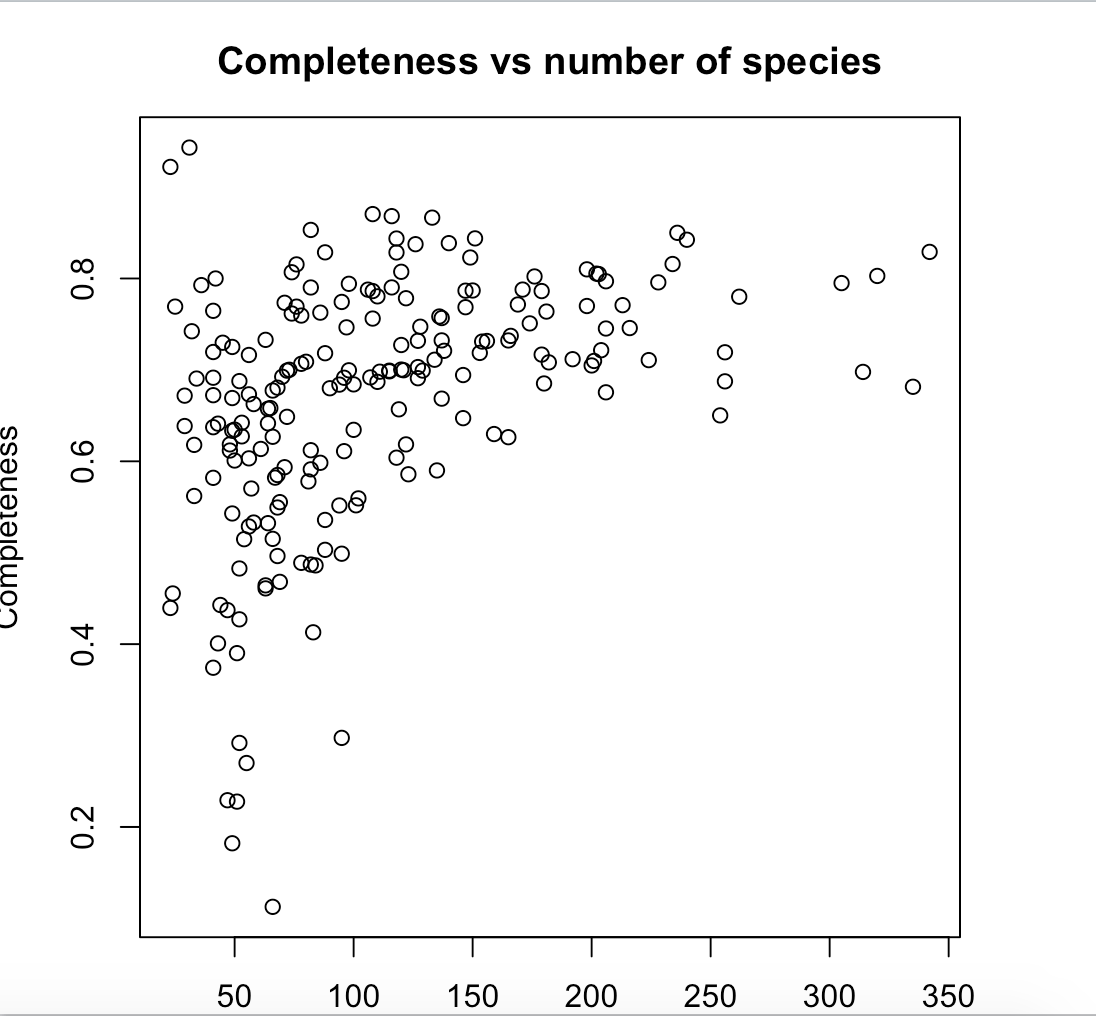
\includegraphics[width=0.5\textwidth]{pictures/biodiversity/complete.jpg} 
      \caption{Completeness}
   \label{fig:completeness}
\end{figure} 

Next use the function mapgrid, which builds a grid map colored according to the density of records in each cell.
Mapgrid allows the user to visually see gap and blank spaces in data.
Grids are 1-degree cells, build with the getcellid function.
Record-density maps apply a color gradient according to the number of records in the cell.
Species-density maps apply a color gradient according to the number of different species in the cell, disregarding the number of records.
Completeness maps apply a color gradient according to the completeness index, from 0 (incomplete) to 1 (complete).
Use the following function to generate a map grid as shown in figure \ref{fig:Mapgrid}

\begin{lstlisting}[morekeywords={mapgrid}]
mapgrid(comp,ptype='complete')
\end{lstlisting}

\begin{figure}[htbp!]
   \centering
   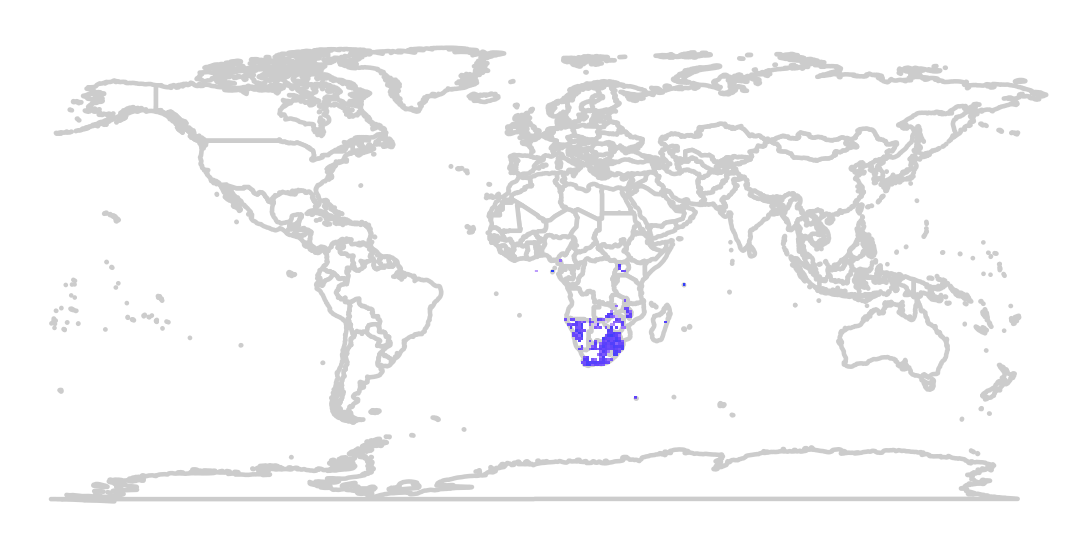
\includegraphics[width=0.5\textwidth]{pictures/biodiversity/map.jpg} 
      \caption{Mapgrid}
   \label{fig:Mapgrid}
\end{figure} 

In order to create a chronohorogram of the dates in the provided data set, use the function chronohorogram.
A chronohorogram plots the number of records on each day with colors indicating the value and concentric circles for each year.
The following code is used to create a chronohorogram like the one shown in figure \ref{fig:chronohorogram}.

\begin{lstlisting}[morekeywords={chronohorogram}]
chronohorogram(birds)
\end{lstlisting}

\begin{figure}[htbp!] 
   \centering
      \caption{Chronohorogram}
   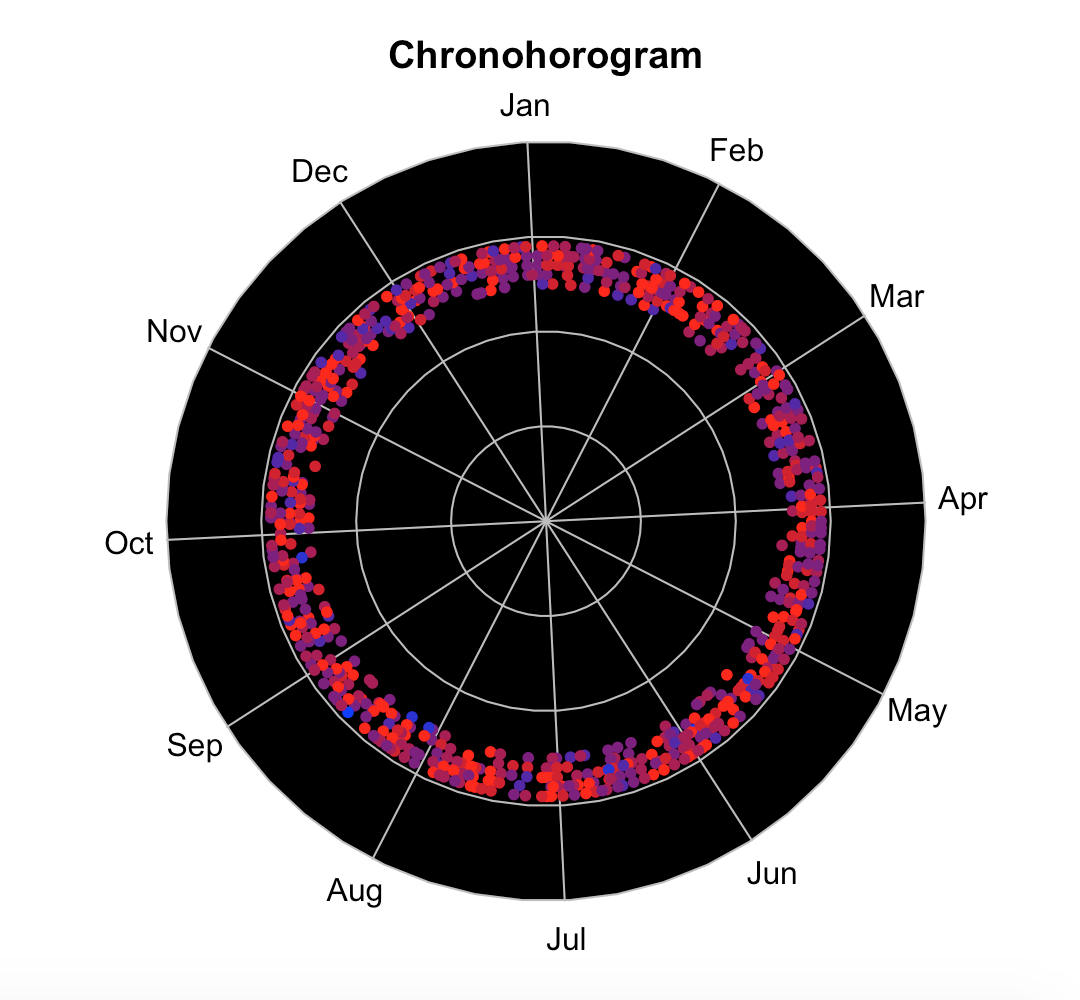
\includegraphics[width=0.5\textwidth]{pictures/biodiversity/chronohorogram.jpg} 
   \label{fig:chronohorogram}
\end{figure} 

Use the function \texttt{distrigraph} to build plots displaying distribution of biodiversity records among user-defined features.
The next four distrigraphs all use different p-types (feature to represent) allowing each graphic to depict different aspects of the data.
The following code is used to create all four distrigraphs respectively as shown in figures \ref{fig:distrigraph1} and \ref{fig:distrigraph2}.

\begin{lstlisting}[morekeywords = {distrigraph,ptype}]
distrigraph(birds,ptype="cell",col="tomato")
distrigraph(birds,ptype="species",ylab="Species")
distrigraph(birds,ptype="efforts",col="red")
distrigraph(birds,ptype="efforts",col="red",type="s")
\end{lstlisting}
\begin{figure}[htbp!]
    \centering
   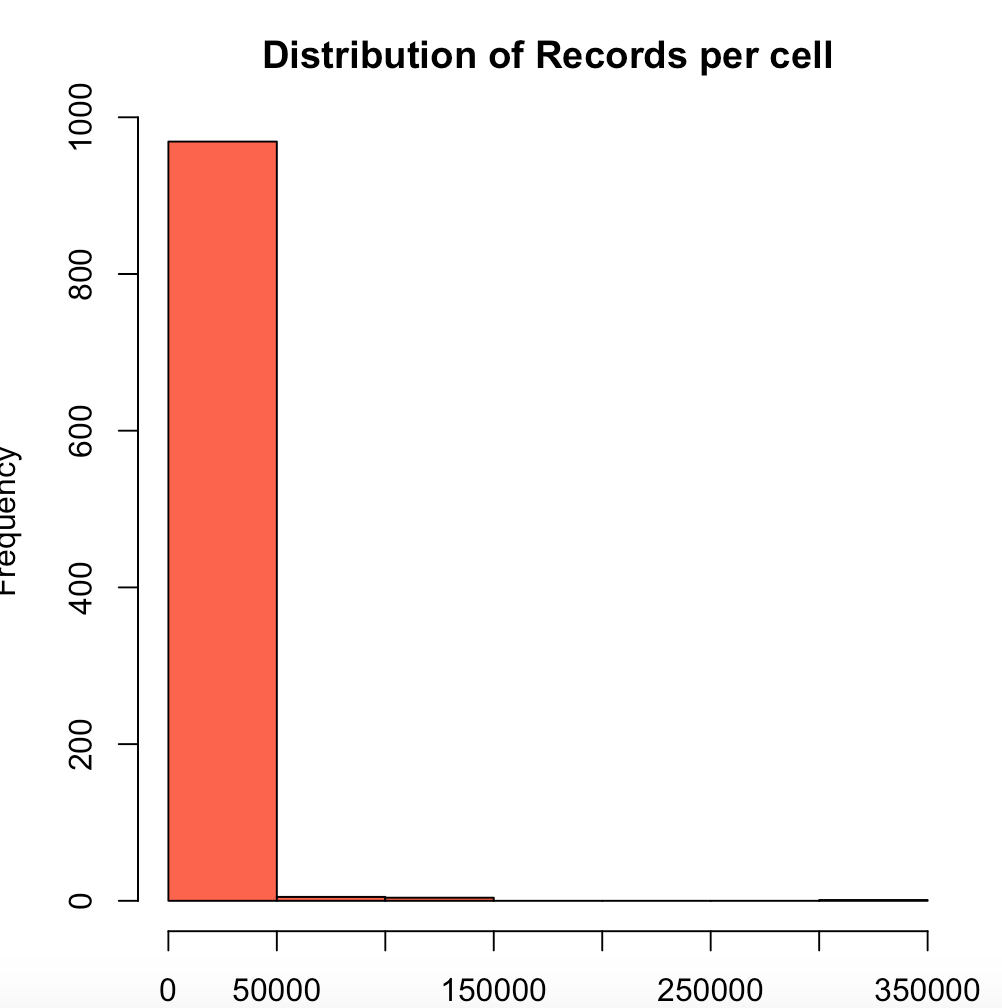
\includegraphics[scale=0.35]{pictures/biodiversity/distrograph1.jpg}
   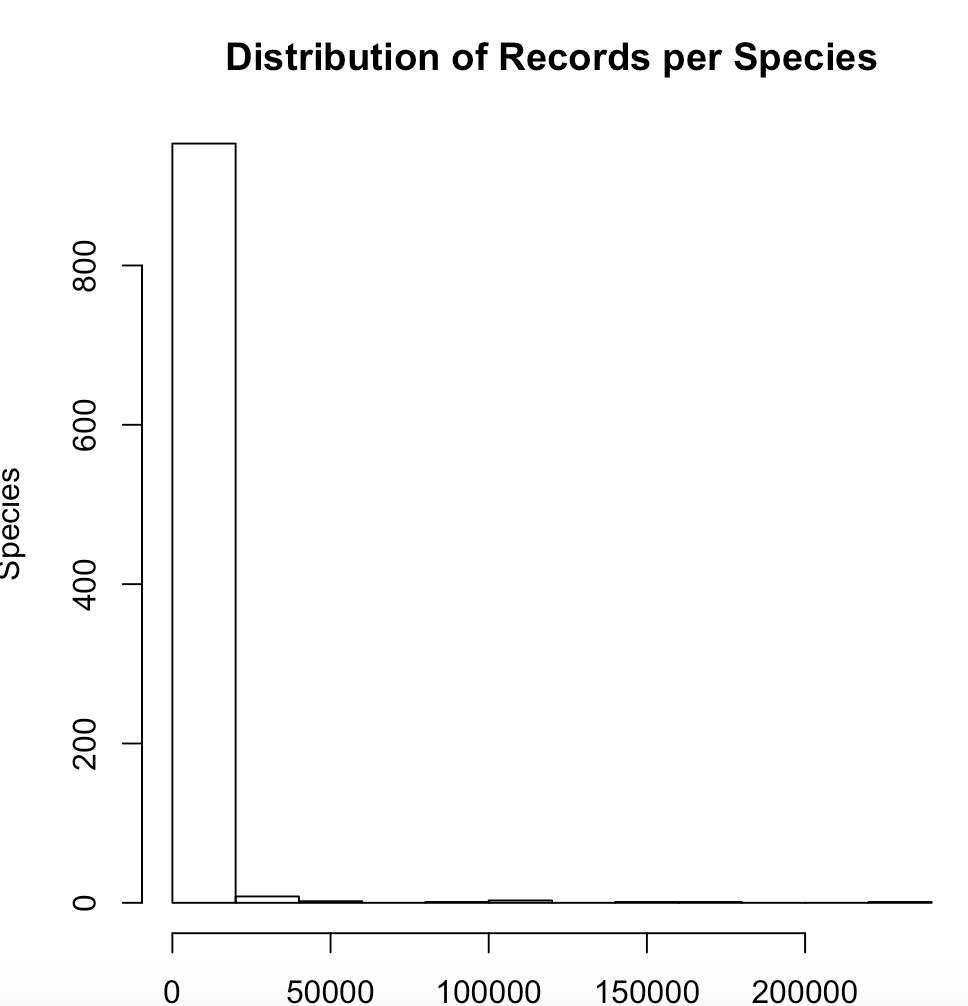
\includegraphics[scale=0.35]{pictures/biodiversity/distrograph2.jpg}
   \caption{Left: Distrigraph 1, Right: Distrigraph 2}
   \label{fig:distrigraph1}
\end{figure}


\begin{figure}[htbp!] 
   \centering
   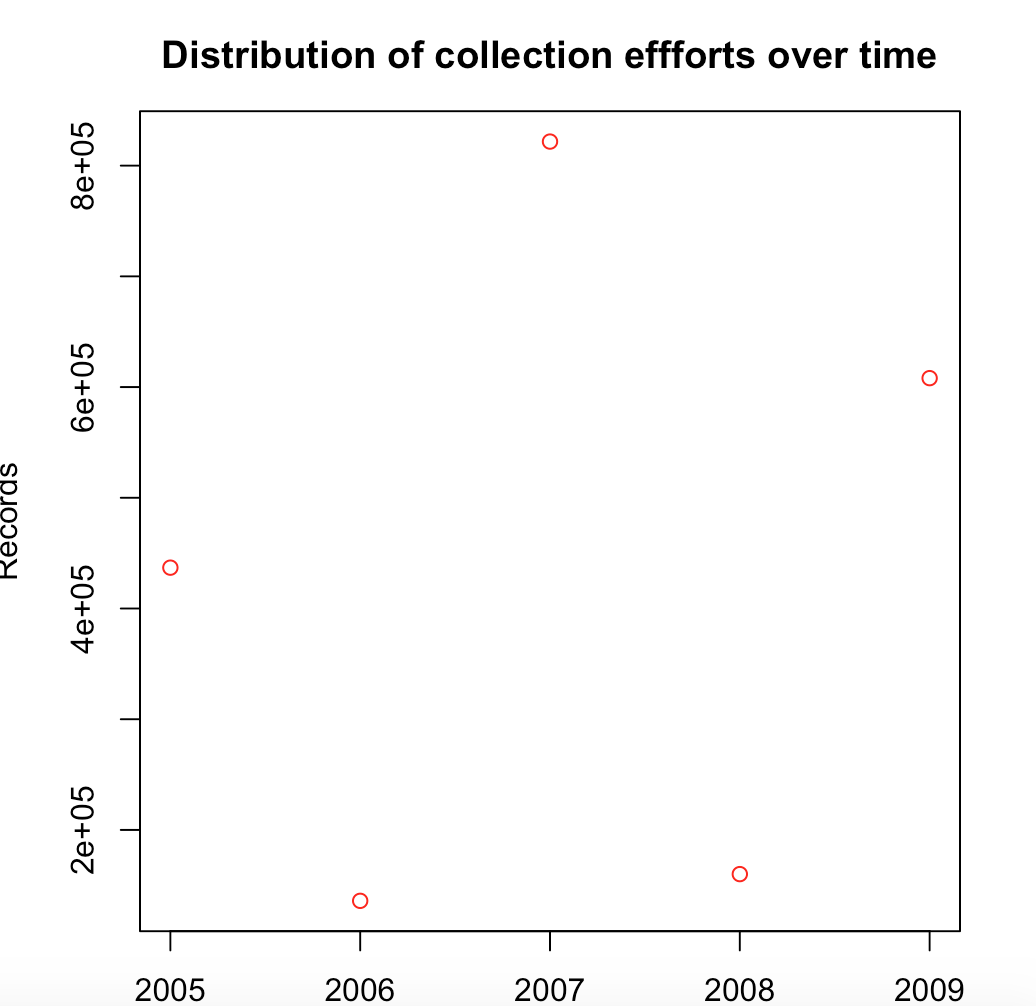
\includegraphics[scale=0.35]{pictures/biodiversity/distrograph3.jpg}
    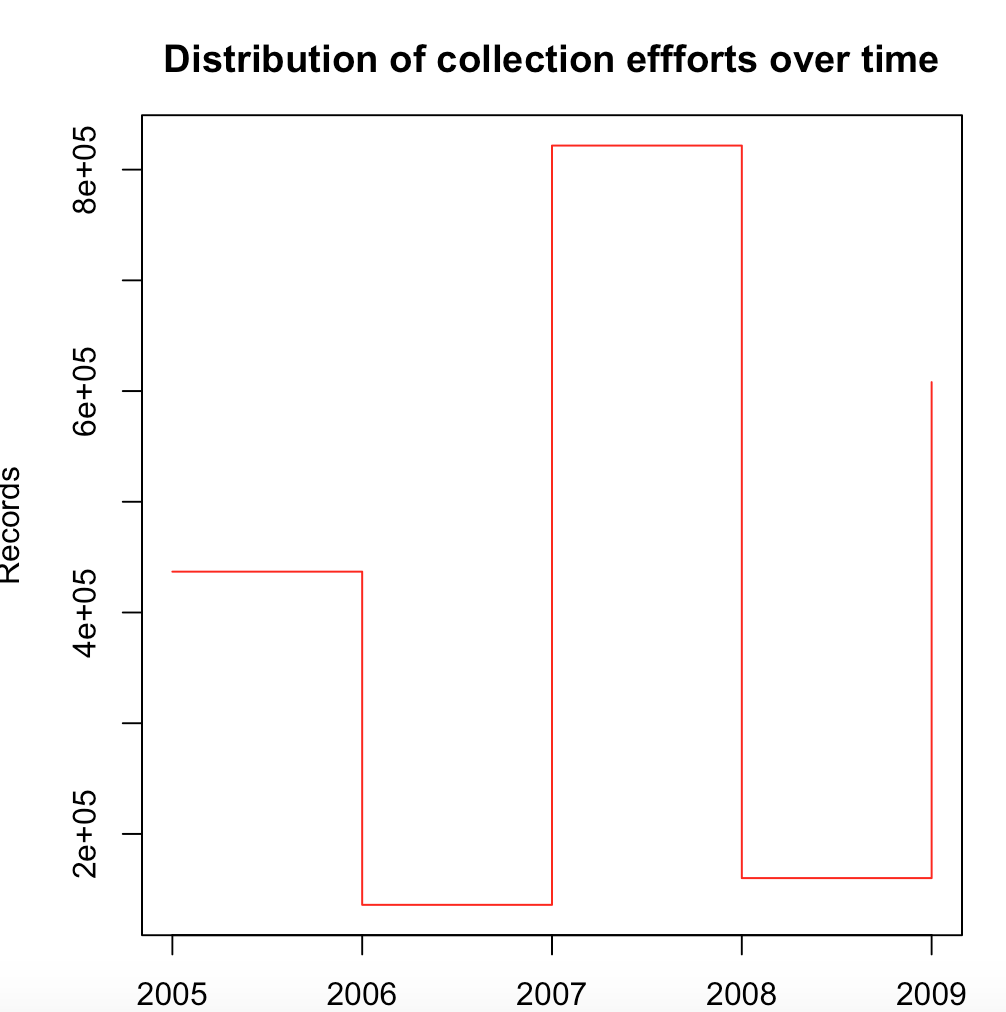
\includegraphics[scale=0.35]{pictures/biodiversity/distrograph4.jpg}
      \caption{Left: Distrigraph 3, Right: Distrigraph 4 }
    \label{fig:distrigraph2}
\end{figure}

\texttt{Bdcalendarheat} creates a calendar heat map in which a calendar is structured as a matrix-like plot where each cell represents a unique date.
The cells are colored as to show the density of records for that date.
Use the following function to create the heat map shown in figure \ref{fig:heatcal}.

\begin{lstlisting}[morekeywords={bdcalendarheat}]
bdcalendarheat(birds)
\end{lstlisting}

\begin{figure}[htbp!] 
   \centering
   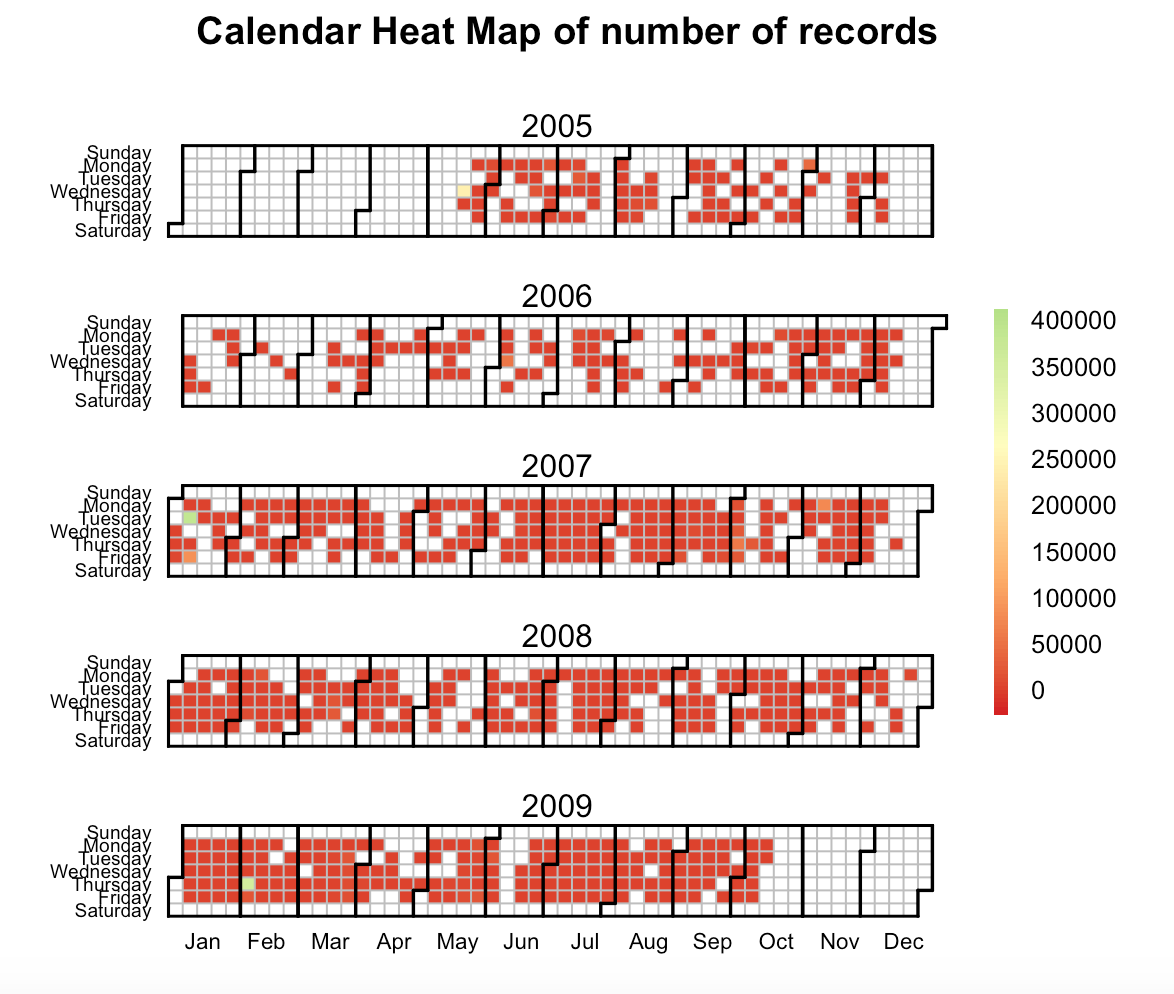
\includegraphics[width=0.5\textwidth]{pictures/biodiversity/heatmap.jpg} 
      \caption{Heat Calendar}
   \label{fig:heatcal}
\end{figure} 

 \subsection{Programming Hints}
 
 Some functions, such as mapgrid, are customizable.
 Arguments within the function, including \texttt{indf}, \texttt{ptype}, \texttt{title}, \texttt{bbox}, \texttt{legscale}, \texttt{collow}, \texttt{colhigh}, \texttt{mapdatabase}, \texttt{region}, and \texttt{customize}, allow the map to be configured to fit the data as desired.
 Using the function \texttt{help()} for mapgrid, and other functions, within the console of RStudio gives a more comprehensive overview of these functions. 
 
 Other functions can be used within the package bdvis.
 These functions include \texttt{tempolar}, \texttt{gettaxo}, and \texttt{taxotree}.
 Each function provides a different view of the data by compiling data that are not used in the other models, and by allowing users to view the same data through different means.
 

\section{Teaching Code}
This is the code shown in the above examples:

\begin{lstlisting}[morekeywords={delim,Latitude,Longitude,config,Date_collected,Scientific_name,bdvis,bdcomplete,chronohorogram,distrigraph,bdcalendarheat,stringsAsFactors,ptype,recs,Scientific,name,Date,collected,mapgrid}]
#set working directory to data location
setwd("/Users/margauxwinter/Desktop/Rfolder/dwca-safring-v1.0")

#read data into RStudio
birds <- read.delim('occurrence.txt', quote='', stringsAsFactors=FALSE)

#configure data
conf <- list(Latitude='decimalLatitude',Longitude='decimalLongitude',
Date_collected='eventDate',Scientific_name='specificEpithet')
birds <- format_bdvis(birds, config=conf)
comp=bdcomplete(birds)

#visualize biodiversity data on the world map
mapgrid(comp,ptype='complete')

#create chronohorogram
chronohorogram(birds) 
comp=bdcomplete(birds,recs=5)

#create various distrigraphs
distrigraph(birds,ptype="cell",col="tomato") 
distrigraph(birds,ptype="species",ylab="Species") 
distrigraph(birds,ptype="efforts",col="red") 
distrigraph(birds,ptype="efforts",col="red",type="s") 

#create heat calendar
bdcalendarheat(birds) 
\end{lstlisting}

\section{Example Student Code}

The final deliverable should be submitted as visual models of the data in the form of distropraphs, maps, chronohorograms, and plots.
Use the arachnid data set downloaded from: \url{http://www.gbif.org/occurrence/download/0012867-160910150852091}

\begin{lstlisting}[morekeywords={delim,Latitude,Longitude,config,Date_collected,Scientific_name,bdvis,bdcomplete,chronohorogram,distrigraph,bdcalendarheat,stringsAsFactors,ptype,timescale,recs,ylab,type,color,Scientific,name,Date,collected,tempolar,mapgrid}]
#set working directory
setwd("/Users/margauxwinter/Desktop/Rfolder/
dwca-arc_national_survey_of_arachnida-v1.1")

#read in data set
spider <- read.delim('occurrence.txt', quote='', stringsAsFactors=FALSE)

#configure data to make it readable for bdvis package
conf <- list(Latitude='decimalLatitude',Longitude='decimalLongitude',
Date_collected='eventDate',Scientific_name='specificEpithet')
spider <- format_bdvis(spider, config=conf)
comp=bdcomplete(spider)

#begin functions for data visualization
mapgrid(comp,ptype='complete')
tempolar(spider, color="green", title="Arachnida daily", plottype="r", timescale="d") 
tempolar(spider, color="blue", title="Arachnida weekly", plottype="p", timescale="w") 
tempolar(spider, color="red", title="Arachnida monthly", plottype="r", timescale="m") 
chronohorogram(spider) 
comp=bdcomplete(spider,recs=5)
distrigraph(spider,ptype="cell",col="tomato") 
distrigraph(spider,ptype="species",ylab="Species") 
distrigraph(spider,ptype="efforts",col="red") 
distrigraph(spider,ptype="efforts",col="red",type="s") 
\end{lstlisting}


\chapterimage{Pictures/ChapterHeadings/header_09.jpg}

	\chapter{HTML Widgets}
        \section{Introduction}
	
	The ability to display statistical data is important in visualizing the information that is generated in scientific studies and research.
        Although \texttt{R} provides a method for visualizing data using graphs and plots, it is often challenging to represent demographic data.
        \texttt{htmlwidgets}, especially the \texttt{leaflet} package, is designed to address this concern.
        Furthermore, \texttt{leaflet} and any other \texttt{htmlwidgets} package can be integrated with \texttt{shiny} to produce a web application that fluidly portrays pertinent information.
	
	\section{Installation}
	
	The following code can be used to install the libraries that will be used in the demonstrations that follow.
	
        \begin{lstlisting}
                > install.packages("shiny")
                > install.packages("leaflet")
        \end{lstlisting}
	
	If the installation results in warnings about the \texttt{R} version you are using, please consider updating for the latest functionality.
	
	The installation, usage, and functionality of \texttt{ShinyApp} is expanded upon separately in another chapter of this R manual. Please consult that section of the book before continuing with the demonstrations outlined in this chapter. Although \texttt{leaflet} can be used in R without \texttt{ShinyApp} integration, the accessibility and functionality of these widgets is best used as a Web application.
	
	\section{Leaflet}
	
	Leaflet is one of the most popular open-source JavaScript libraries for interactive maps.
        It is used by websites ranging from The New York Times and The Washington Post to GitHub and Flickr, as well as GIS specialists like OpenStreetMap, Mapbox, and CartoDB \cite{leaflet}.
        The Leaflet libraries have been integrated fluidly into a R widget package form. We will learn the basics about this widget by creating some simple demonstrations.
	
	\subsection{Leaflet Demonstration 1 - A Simple Map}
	
	We can develop a simple user interface for our \texttt{ShinyApp} integration.
        Include a title panel, and create a sidebar layout.
        For this demonstration, we will simply have two numeric input controls that allow the user to enter the latitude and longitude.
        Our \texttt{ShinyApp} server will automatically render the new position onto the Leaflet map.
	
        \begin{lstlisting}
        library(shiny)
        library(leaflet)
        
        ### USER INTERFACE ###
        
        ui <- fluidPage(
                # Title of the ShinyApp
                titlePanel("Leaflet Demonstration 1"),
                # A layout with a sidebar
                sidebarLayout(
                        # Content of the sidebar panel
                        sidebarPanel(
                                # Two input controls
                                numericInput("lat", "Latitude:", min=-90, max=90, value=44.366002, step=0.001),
                                numericInput("lon", "Longitude:", min=-180, max=180, value=-68.196409, step=0.001)
                        ),
                        # Content of the main panel
                        mainPanel(
                                # The leaflet widget UI
                                leafletOutput("map")
                        )
                )
        )
        \end{lstlisting}

	For the server-side logic, we simply render the leaflet using a reactive system so that every time the latitude or longitude is updated, the map renders itself again. We generate a \texttt{leaflet()} object and assign it certain attributes from functions that are provided by the \texttt{leaflet} package. The \texttt{addTiles()} command ensures that the map will use the default map tiles that are provided in the package. The \texttt{addMarkers()} command adds a marker on the map that points to the location that has been chosen. This command also supports multiple markers in one command.
	
        \begin{lstlisting}
        ### SERVER LOGIC ###
        
        server <- function(input, output) {
                # Set the output map using a rendering function
                output$map <- renderLeaflet({
                        # The leaflet object
                        leaflet() %>%
                                addTiles() %>%
                                addMarkers(lng=input$lon, lat=input$lat, popup="The Location")
                })
        }
        \end{lstlisting}	
	
	Finally, we run the server using the \texttt{shinyApp()} command.
        We pass both the user interface and the server logic as arguments.
        The server will run on a local address, such as \texttt{http://127.0.0.1:7591}. 
	
        \begin{lstlisting}
        shinyApp(ui=ui, server=server)
        \end{lstlisting}

	Running the server produces an interactive map with a marker at the location that has been specified with the latitude and longitude in the sidebar.
        By changing the values, we can change the location reactively.
        Furthermore, we can zoom in and out of the map using the scroll function or the buttons provided on the map.
        Finally, we can also drag around the map by clicking inside the map control.
	
	\begin{figure}[htbp!]
		\centering
		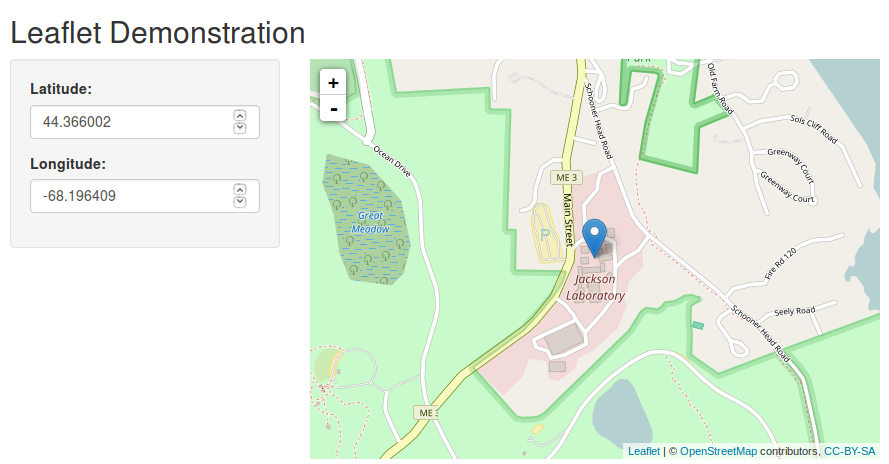
\includegraphics[width=12cm]{pictures/html/htmlwidgets-image-1.png}
		\caption{The Result of our First Demonstration}
	\end{figure}

	\subsection{Leaflet Demonstration 2 - Map Tiles}
	
	In this section, we will explore the different views and tiles that are provided by third-party developers.
        We will only be changing the part of the code that renders the \texttt{leaflet()} in the server logic.
        The \texttt{setView()} command allows us to choose the location of the initial view and the level of zoom.
	
        \begin{lstlisting}
        # Stamen.Toner
        output$map <- renderLeaflet({
                leaflet() %>%
                        addProviderTiles("Stamen.Toner") %>%
                        setView(lng=-71.0589, lat=42.3601, zoom=12)
        })
        # CartoDB.Positron
        output$map <- renderLeaflet({
                leaflet() %>%
                        addProviderTiles("CartoDB.Positron") %>%
                        setView(lng=-71.0589, lat=42.3601, zoom=12)
        })
        \end{lstlisting}

	\begin{figure}[htbp!]
		\centering
		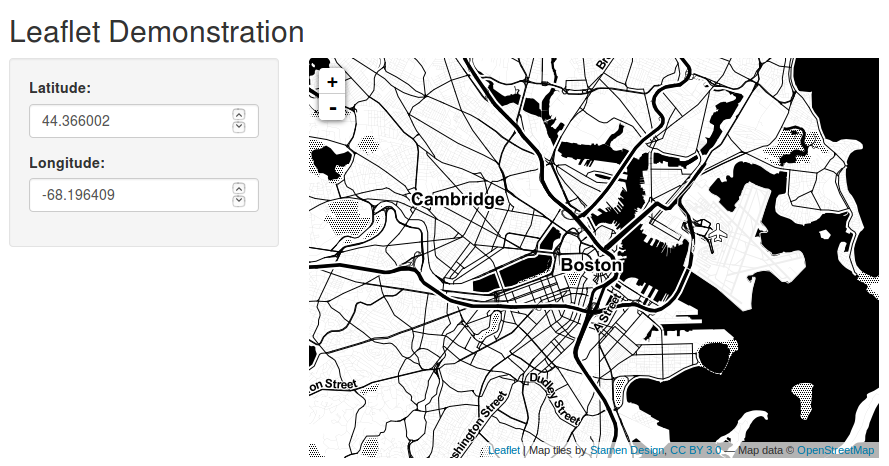
\includegraphics[width=.5\textwidth]{pictures/html/htmlwidgets-image-2.png}
		\caption{The Toner Tiles}
	\end{figure}

	\begin{figure}[htbp!]
		\caption{The Positron Tiles}
		\centering
		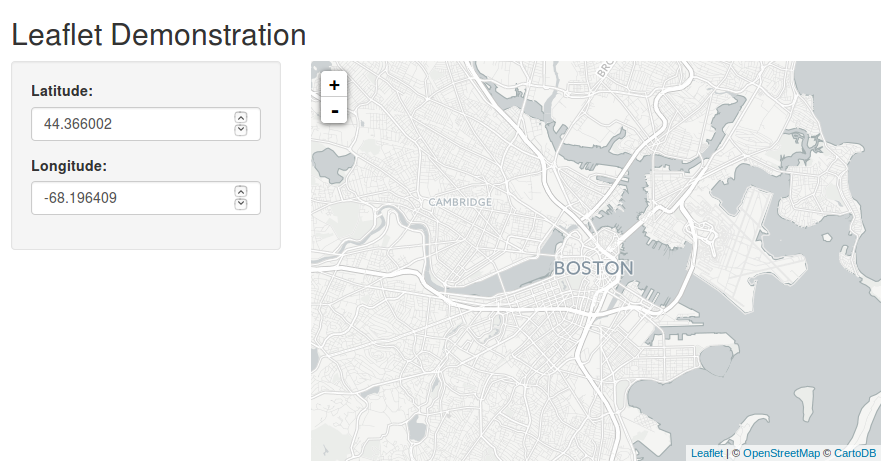
\includegraphics[width=.5\textwidth]{pictures/html/htmlwidgets-image-3.png}
	\end{figure}

	\subsubsection{Web Map Service Tiles}
	
	We can use interesting commands to overlay the graphics from other web map services onto our tiles.
        For example, we will create a map that shows the intensity of precipitation by using the \texttt{addWMSTiles()} command.
	
        \begin{lstlisting}
        output$map <- renderLeaflet({
                leaflet() %>%
                        addTiles() %>%
                        setView(-93.65, 42.0285, zoom=4) %>%
                        addWMSTiles(
                                "http://mesonet.agron.iastate.edu/cgi-bin/wms/nexrad/n0r.cgi",
                                layers = "nexrad-n0r-900913",
                                options = WMSTileOptions(format = "image/png", transparent = TRUE),
                                attribution = "Weather data Copyright 2012 IEM Nexrad"
                        )
        })
        \end{lstlisting}

	\begin{figure}[htbp!]
		\centering
		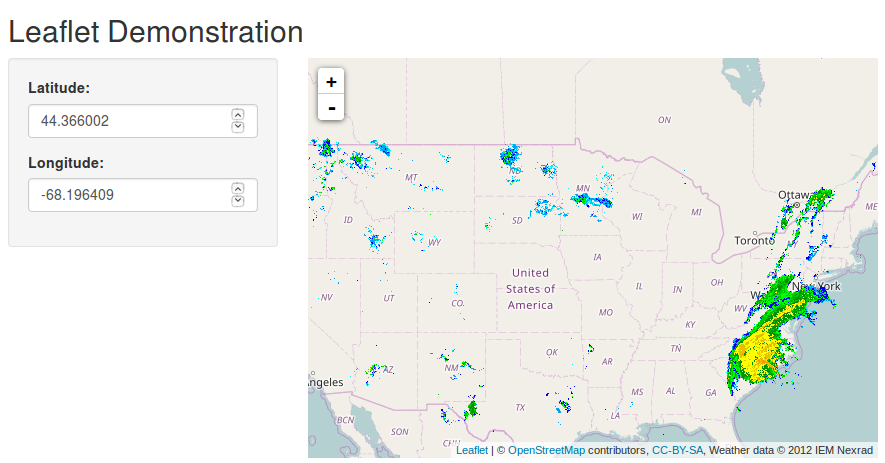
\includegraphics[width=.5\textwidth]{pictures/html/htmlwidgets-image-4.png}
		\caption{The Weather Data for Precipitation}
	\end{figure}

	\subsection{Leaflet Student Demonstration - Markers}
	
	One of the most important functions of this widget, and this chapter in general, is the ability to correctly visualize data.
        To accomplish this, we utilize markers, which are inconsequential to visualizing data on maps.
        We will use population data from some major cities in America and use different markers to visualize the data.
	
	\noindent\textbf{Student Prompt: } Use the following code that provides population data to develop a map that accurately demonstrates the size of each city mentioned in the dataset.
		
        \begin{lstlisting}
                population <- read.csv(textConnection(
                "City,Population,Lat,Lon,
                        Nashville,678889,36.1627,-86.7816
                        Asheville,87236,35.5951,-82.5515
                        Portland,609456,45.5231,-122.6765
                        Denver,649495,39.7392,-104.9903
                        Kansas City,467007,39.0997,-94.5786
                        Seattle,652405,47.6062,-122.3321
                        New York City,8406000,40.7128,-74.0059"
                ), header=TRUE)
        \end{lstlisting}

	\noindent\textbf{Solution}
	
	In general, after using the documentation found on the web, most students will create a solution as follows:

        \begin{lstlisting}
        server <- function(input, output) {
                
                output$map <- renderLeaflet({
                        leaflet(data=population) %>%
                                addTiles() %>%
                                addMarkers(~Lon, ~Lat, popup=~paste(sep="<br/>", paste(sep="", "<b>", as.character(City), "</b>"), as.character(Population)))
                })
        }
        \end{lstlisting}

	The code will generate the following maps.
        Unfortunately, this type of visualization, while informative about the location of every city, does not help visualize any part of the population in every location.
        We will instead try to create a visual representation of the population in every location by generating circles with an area proportional to the population of the city.
	
	\begin{figure}[htbp!]
		\centering
		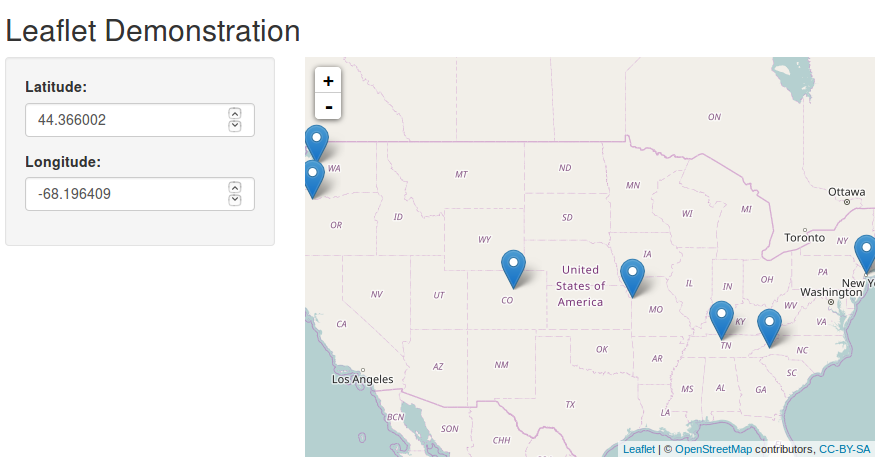
\includegraphics[width=12cm]{pictures/html/htmlwidgets-image-5.png}
		\caption{The Markers Placed at Every Location}
	\end{figure}

	The \texttt{addCircleMarkers()} allows us to add circles that have custom properties depending on the data point.
        We will use the \texttt{radius} attribute to make the circle larger or smaller depending on the population of the city.
	
        \begin{lstlisting}
        output$map <- renderLeaflet({
                leaflet(data=population) %>%
                        addTiles() %>%
                        addCircleMarkers(~Lon, ~Lat, popup=~paste(sep="<br/>", paste(sep="", "<b>", as.character(City), "</b>"), as.character(Population)), radius=~sqrt(Population/1000))
        })
        \end{lstlisting}
	
	\begin{figure}[htbp!]
		\centering
		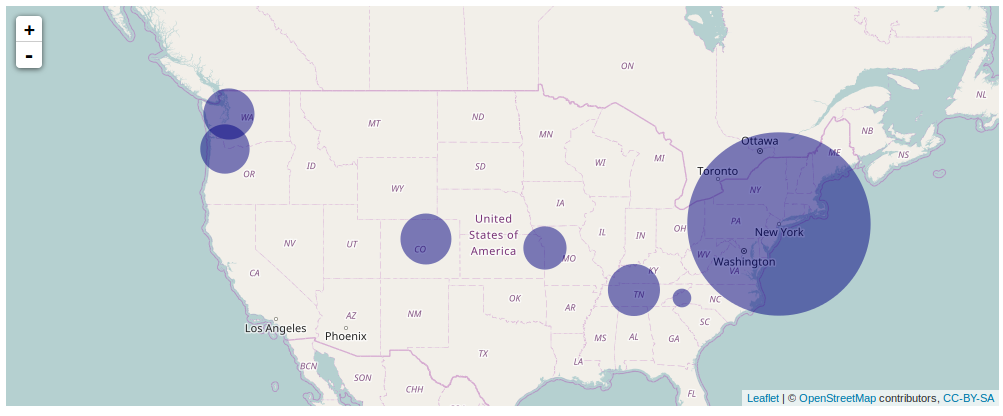
\includegraphics[width=.5\textwidth]{pictures/html/htmlwidgets-image-6.png}
		\caption{The Markers Placed at Every Location}
	\end{figure}


\chapterimage{Pictures/ChapterHeadings/header_10.jpg}

\chapter{Estimating Pi Using Monte~Carlo Simulations}
\section{Introductory Reading}
$\pi$ (pi) denotes the ratio of the circumference of a circle to its diameter and is of great importance in mathematics.
The first to attempt a theoretical calculation of its value was Archimedes \cite{smoller}, who was able to prove the following inequality:
\[
\frac{223}{71} < \pi < \frac{22}{7}
\]
In recent years, supercomputers have been able to calculate pi to 13.3 trillion digits \cite{yee}.
In this lesson, we investigate a computational method that can be used roughly determine the value of $\pi$: the Monte Carlo Method \cite{andersson}.

\noindent 
The Monte Carlo method is based on geometric probability.
A circle inscribed in a square of side length 2 will have an area of $\pi$.
Thus, the probability that any random point in the square is also inside the circle will be $\frac{\pi}{4}$.
We can approximate $\pi$ by asking the computer to pick a large number of random points inside the square, and seeing how many are also inside the circle.

\noindent 
We will use the Shiny package to display a plot with the circle inscribed in a square.
We will also output the numerical approximation of $\pi$.

\section{Objectives of the Case Study}
\begin{itemize}
\item
Students will use the Shiny package to create a Monte Carlo simulation in R.
\item
Students will understand the mathematical basis behind the estimation of $\pi$ program.
\item
Students will use their Monte Carlo program to approximate the value of $\pi$.
\end{itemize}
\section{Building the Model}

The Monte Carlo simulation will be built using the Shiny package in R.
This package is used to interactively display outputs such as plots and histograms.
Today, we will be using it to display a plot of the circle inscribed in the square, as well as outputting the value of the $\pi$ approximation.

\noindent 
To begin the application, open a new R script file in RStudio, clear the environment, set a working directory, and import the libraries necessary for this project.
To clear the environment and set a directory use the following functions.
Make sure you set a directory on your computer that the dataset is located in. 

\begin{lstlisting}
rm(list=ls())
setwd("C:/Users/Ishaan/Documents/NCSSM 2015-2016")
\end{lstlisting}

\noindent The libraries are as follows:

\begin{lstlisting}
library(shiny)
library(plotrix)
\end{lstlisting}


\noindent 
If you don't have one of these libraries installed on your computer, you can simply type \texttt{install.packages("insertlibraryname")} in the console to download them.

\noindent 
To begin, we will initialize the basic Shiny outline with the following code.
Shiny relies on developing outputs based on any user input.

\begin{lstlisting}
    server <- function(input, output) {
    
    }
    
    ui <- shinyUI(fluidPage(
        headerPanel("Estimating Pi"),
        sidebarPanel(),
        mainPanel()
    ))
    
    shinyApp(ui = ui, server = server)
\end{lstlisting}

\noindent 
This is the skeletal structure of the simplest Shiny application possible.
Run the Shiny application by selecting all of your code and clicking the run button in the top right corner of RStudio.
The blank Shiny application should open in a new window and look like figure \ref{fig:blankshiny}.

\begin{figure}[htbp!]
   \centering
   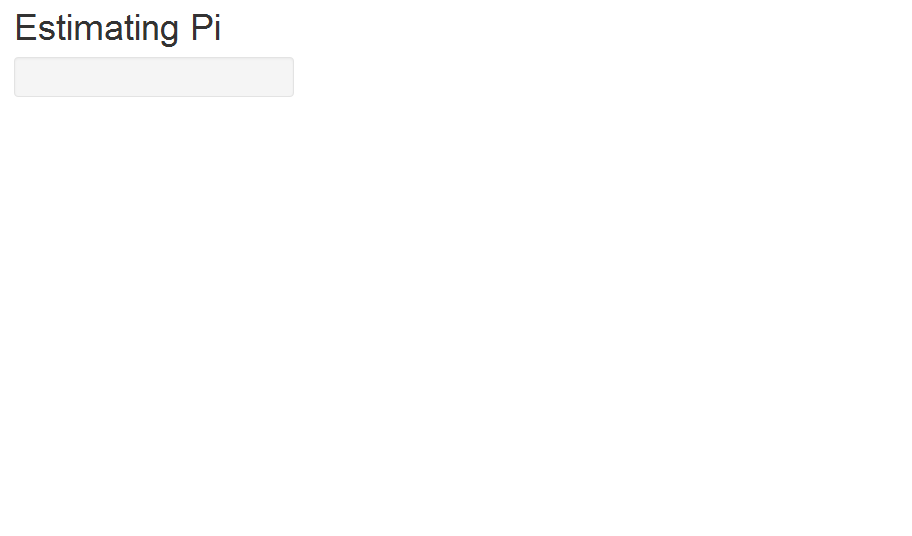
\includegraphics[width = .5\textwidth]{pictures/pi/blank2.PNG} 
   \caption{Blank Shiny App}
   \label{fig:blankshiny}
\end{figure}

\noindent 
To begin the model, we need to display the inputs of our program in the sidebar panel of the application.
Our program is only taking in one input: number of simulated points.
This input will define how many points the Monte Carlo method will simulate on the plot.
We can do this like so:

\begin{lstlisting}
    sidebarPanel(
        numericInput(inputId = "simulate", "Number of Simulated Points:",
        100, min = 100, max = 10000)
    )
\end{lstlisting}
 
 \noindent 
 This block of code will take a numerical value between $100$ and $10000$ as the number of simulated points.
 We want to set a maximum of $10000$, because if we run more than $10000$ simulations, the code because very computationally intensive and could result in RStudio crashing or your computer freezing.
 The \texttt{inputId} is simply a name we give the value of the input for future reference. 
 
 \noindent 
 We also need to tell the application that our plot will be displayed in the main panel of the user interface.
 We also want the value of $\pi$ that we have estimated to appear on the page.
 This involves creating a \texttt{plotOutput} and a \texttt{textOutput}, like so:

\begin{lstlisting}
 mainPanel(
    textOutput(outputId = "estimate"),
    plotOutput(outputId = "monte", width = "400px", height = "400px")
 )
\end{lstlisting}

\noindent 
Just like in \texttt{selectInput}, we need to give the outputs an ID, so we can use that name to access it in the server function.
Once the model is run, the application should look like figure \ref{fig:appwithinputs}. 

\begin{figure}[htbp!]
   \centering
   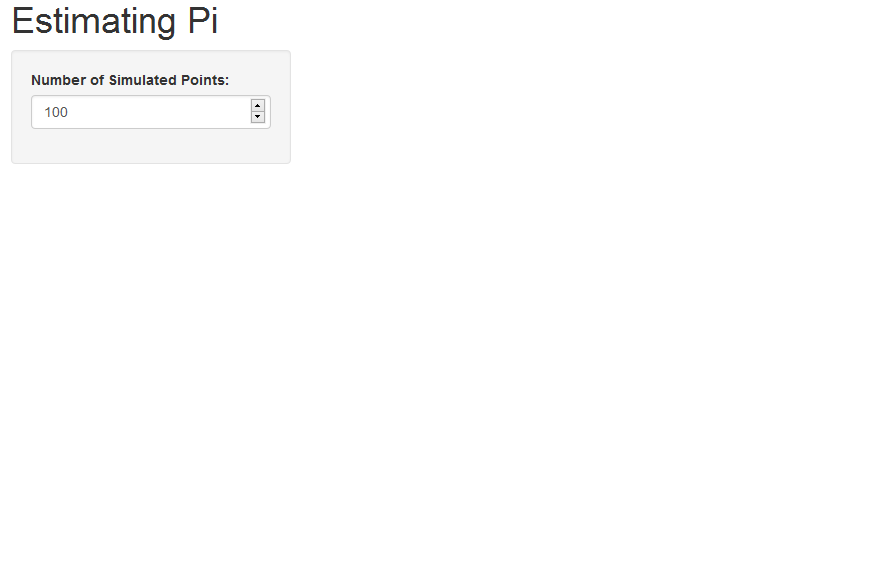
\includegraphics[width=.5\textwidth]{pictures/pi/input.PNG} 
   \caption{Shiny App with Inputs}
   \label{fig:appwithinputs}
\end{figure}
 
\noindent
Next we need to define the server-side of the application which will accept inputs and compute outputs.
Our server function will contain the code necessary to do this.
We first tell the function that we are creating a plot as an output, and we can create these outputs using the \texttt{renderPlot} and \texttt{renderText} command.

\begin{lstlisting}
    output\$monte <- renderPlot({
        
    })
    
    output\$estimate <- renderText({
    
    })
\end{lstlisting}
 
\noindent The goal of this program is to simulate hundreds points on a plot of a unit circle circumscribed in a square.
We need to generate x and y coordinates for these points, and then check if they fall within the circle.
To do this we will use the \textit{runif} command.
This command generates random deviates within a range of values for a certain number of observations.

\noindent We will set two variables, \texttt{x} and \texttt{y}, to store the \texttt{x} and \texttt{y} coordinates of the generated points.
Remember we want these values to lie between $-1$ and $1$ on the coordinate grid.
We want to run this simulation within the \texttt{renderPlot} and \texttt{renderText} functions so both outputs can access the result.
This can be done like so: 

\begin{lstlisting}
    output\$monte <- renderPlot({
        x <- runif(input\$simulate, min = -1, max = 1)
        y <- runif(input\$simulate, min = -1, max = 1
    })
    
    output\$estimate <- renderText({
        x <- runif(input\$simulate, min = -1, max = 1)
        y <- runif(input\$simulate, min = -1, max = 1
    })
   
\end{lstlisting}

\noindent The \texttt{input\$simulate} term is the number of simulations that the user inputs into the model.
This function will generate values between $-1$ and $1$ and store them in the \texttt{x} variable.
Now we have to test if these points lie within the circle. The equation of a circle is $x^{2}$ + $y^{2}$ = $r^{2}$.
This can be done using the \texttt{s.inside} command, which returns a $1$ or $0$ depending on if the point is inside the given boundary.
Then we want to find the ratio of the number of points within the circle to the number of total points and multiply this by $4$ to get an estimation of $\pi$. 

\begin{lstlisting}
     output\$monte <- renderPlot({
        x <- runif(input\$simulate, min = -1, max = 1)
        y <- runif(input\$simulate, min = -1, max = 1
        is.inside <- (x^2 + y^2) <= R^2
        estimation <- 4*sum(is.inside) / N
    })
    
    output\$estimate <- renderText({
        x <- runif(input\$simulate, min = -1, max = 1)
        y <- runif(input\$simulate, min = -1, max = 1
        is.inside <- (x^2 + y^2) <= R^2
        estimation <- 4*sum(is.inside) / N
    })
\end{lstlisting}

\noindent All we need to do now is to output the value of our estimation as well as the plot of the circle and the square.
To output the text, we can simply use a return function within the renderText environment under the rest of our code like so: 

\begin{lstlisting}
    return(c("Estimate of Pi:", estimation))
\end{lstlisting}
 
\noindent To plot the circle and the points, we use the \texttt{plot} command to place the randomly generated points on a grid, and use the \texttt{draw.circle} command to draw a circle.
To highlight which points are inside the circle we can color them blue, and the ones not inside will be colored red. 

\begin{lstlisting}
    plot(x, y, asp=1, xlim = c(-1,1), ylim = c(-1,1))
    draw.circle(0,0,1,nv=1000,lty=1,lwd=1)
    points(x[ is.inside], y[ is.inside], pch = 19, col = "blue")
    points(x[!is.inside], y[!is.inside], pch = 19, col = "red")
\end{lstlisting}

\noindent The above code should go in the \texttt{renderPlot} command under the previous code.
Now when the Shiny app is run your final project should like figure \ref{fig:Complete}. 

\begin{figure}[htbp!]
   \centering
   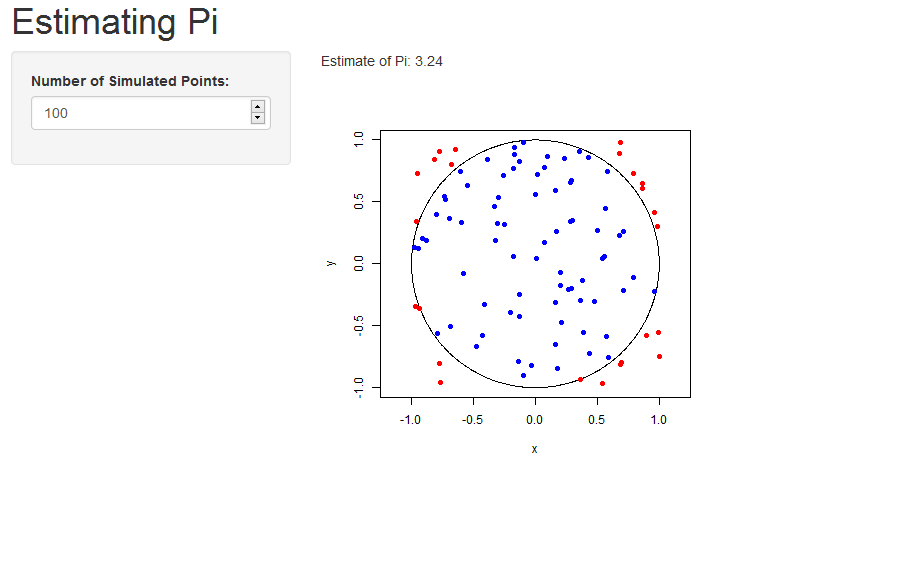
\includegraphics[width=0.5\textwidth]{pictures/pi/estimate.PNG} 
   \caption{Complete Estimating Pi Application}
   \label{fig:Complete}
\end{figure}

\noindent Your application is now complete!
Feel free to explore the approximations of $\pi$ as you increase or decrease the number of simulated points. 

\section{Deliverable}

For the final deliverable, the student should submit their code, along with a screenshot of the Shiny application using an instructor-defined number of simulated points.

\section{Teaching Code}

Students may use the framework below as a guide:

\begin{lstlisting}
#Student name
#Date
#EstimatingPi.R

#clean up and set the directory


#load libraries


#setting the server, code instructing R what to do with inputs


    #initialize objects
   
    
    #create plot
    
  
  #set up estimate routine  
  

#create graphics


#call shiny app


\end{lstlisting}

\section{Example Student Code}

The code that students submit should be similar to the example given below:

\begin{lstlisting}
#Ishaan Rao
#September 1, 2016
#EstimatingPi.R

#clean up and set the directory
rm(list=ls())
setwd("C:/Users/Ishaan/Documents/NCSSM 2015-2016")

#load libraries
library(shiny)
library(plotrix)

#setting the server, code instructing R what to do with inputs
server <- function(input, output) {
  output\$monte <- renderPlot({
    
    N <- input\$simulate
    R <- 1
    x <- runif(N, min = -R, max = R)
    y <- runif(N, min = -R, max = R)
    is.inside <- (x^2 + y^2) <= R^2
    estimation <- 4*sum(is.inside) / N
    
    #plot.new()
    #plot.window(xlim = 1.1 * R * c(-1, 1), ylim = 1.1 * R * c(-1, 1))
    plot(x, y, asp=1, xlim = c(-1,1), ylim = c(-1,1))
    draw.circle(0,0,1,nv=1000,lty=1,lwd=1)
    points(x[ is.inside], y[ is.inside], pch = 19, col = "blue")
    points(x[!is.inside], y[!is.inside], pch = 19, col = "red")
  })
  
  output\$estimate <- renderText({
    N <- input\$simulate
    R <- 1
    x <- runif(N, min = -R, max = R)
    y <- runif(N, min = -R, max = R)
    is.inside <- (x^2 + y^2) <= R^2
    estimation <- 4*sum(is.inside) / N
    
    return(c("Estimate of Pi:", estimation))
    
  })
}

ui <- shinyUI(fluidPage(
  headerPanel("Estimating Pi"),
  sidebarPanel(
    numericInput("simulate", "Number of Simulated Points:", 100, min = 100, max = 10000)
  ),
  mainPanel(
    textOutput("estimate"),
    plotOutput("monte", width = "400px", height = "400px")
  )
))

shinyApp(ui = ui, server = server)

\end{lstlisting}

\section{Further Readings}

To learn more about what Monte Carlo simulations are and their applications to a wide variety of problems visit \url{https://en.wikipedia.org/wiki/Monte\_Carlo\_method} or 
\url{http://www.palisade.com/risk/monte\_carlo\_simulation.asp}.

\noindent To learn more about the mathematical theory behind estimating $\pi$ visit \url{https://en.wikipedia.org/wiki/Approximations_of_\%CF\%80} or \url{http://polymer.bu.edu/java/java/montepi/MontePi.html}


\chapterimage{Pictures/ChapterHeadings/header_11.jpg}

\chapter{Plotluck}
\section{Introduction}
Coined as the ``ggplot2 version of `I'm feeling lucky!''', \texttt{plotluck} is designed to consider the characteristics of a data frame to decide, through a heuristic algorithm, the most appropriate plot to represent the data.
The package has scatter, box, bar, violin, density, heat map, hexagon bin, and spine plots available.
The ultimate goal of the package is to allow users to explore which type of plot would best fit their data, instead of becoming burdened with the creating code in R.

\section{Objectives}
In this assignment, we will use \texttt{plotluck} to explore rapid visualization of several data sets.
The code created is a good place to start, but we encourage you to continue exploring the package.
The website Gapminder has an extreme amount of data sets available for public use, and R has around 30 data sets built in.

\section{Deliverable}
As plot luck is created for finding and forming appropriate graphics for respective data sets, the desired deliverable will be dependent on the data set used.

For example, plots using ggplot2's \texttt{mpg} data set are shown in figures \ref{fig:mpg1}, \ref{fig:mpg2}, and \ref{fig:mpg3}.

\begin{figure}[htbp!]
    \centering
    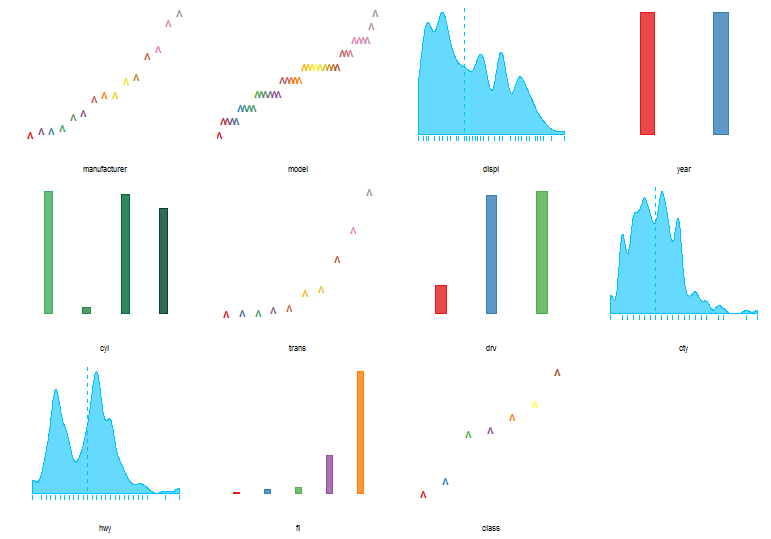
\includegraphics[width=.5\textwidth]{pictures/plotluck/mpgall}
    \caption{Plotting every variable in \texttt{mpg}}
    \label{fig:mpg1}
\end{figure}

\begin{figure}[htbp!]
    \centering
    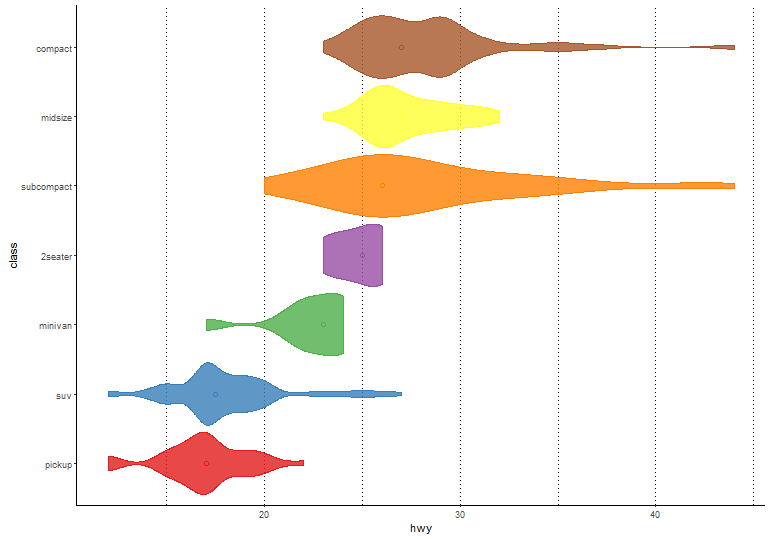
\includegraphics[width=.5\textwidth]{pictures/plotluck/mpg1}
    \caption{Highway mileage to class}
    \label{fig:mpg2}
\end{figure}

\begin{figure}[htbp!]
    \centering
    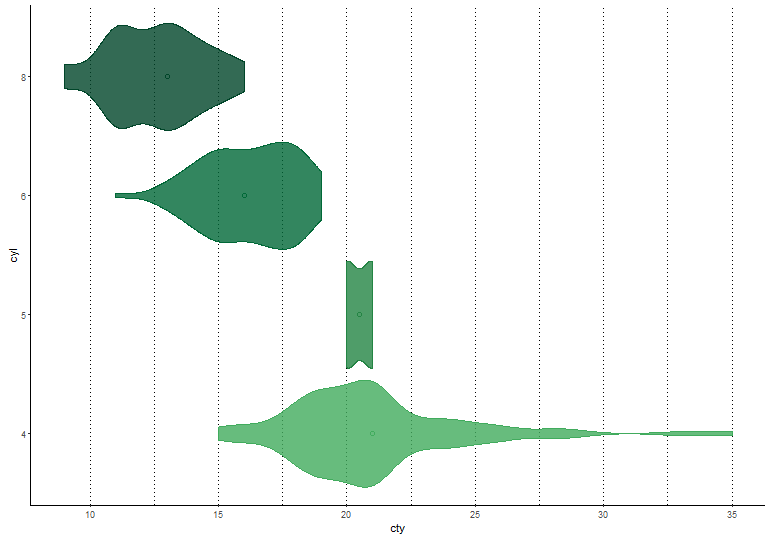
\includegraphics[width=.5\textwidth]{pictures/plotluck/mpg2}
    \caption{Cylinder count vs city mileage}
    \label{fig:mpg3}
\end{figure}

More examples include figures \ref{diamondprice} and \ref{txhousing}.

\begin{figure}[htbp!]
    \centering
    \includegraphics[width=.5\textwidth]{pictures/plotluck/diamonds1}
    \caption{Price to color in the \texttt{diamonds} dataset}
    \label{diamondprice}
\end{figure}

\begin{figure}[htbp!]
    \centering
    \includegraphics[width=.5\textwidth]{pictures/plotluck/txhousingall}
    \caption{Plotting every variable in \texttt{txhousing}}
    \label{txhousing}
\end{figure}

\section{Teaching Code}
\begin{lstlisting}
# Example for Plotluck

# Clean up and import plotluck
rm(list=ls())
library(plotluck)
setwd("C:/Your/R/Directory")

# Let's work with the faithful data
# What's in this data set?
plotluck(.~1, faithful)

# Look at everything vs everything else:
plotluck(.~., faithful)

# Eruptions look interesting, what can that tell us?
plotluck(eruptions~., faithful)
plotluck(eruptions~waiting, faithful)

# Let's look at airquality
plotluck(.~1, data=airquality)

# We can generate some interesting plots because Month is discrete
plotluck(Temp~Month, airquality)
plotluck(Wind~Month, airquality)
plotluck(Ozone~Month, airquality)

# And some more interesting ones
plotluck(Temp~Solar.R+Ozone, airquality)
plotluck(Temp~Wind+Ozone, airquality)
plotluck(Temp~Solar.R|Month, airquality)

# Let's look at mtcars
# This tells us more about the variables
plotluck(.~1, mtcars)
# Here are some interesting examples
plotluck(vs~gear, mtcars)
plotluck(mpg~wt, mtcars)

# Let's explore random plotting!
data(diamonds, package='ggplot2')
set.seed(100)
# Run this several times to get random plots
sample.plotluck(diamonds)
# Note the following hex plots:
plotluck(depth~x, diamonds)
plotluck(price~carat, diamonds)

\end{lstlisting}

\section{Example Student Code}
\begin{lstlisting}
# EXAMPLE KEY
# Date
# Plotluck Exercises - KEY

# Clean up and import plotluck
rm(list=ls())
library(plotluck)
setwd("D:/School/RCompSci/book/plotluck")

# Using the following command:
# data(dataset_name, package='ggplot2')
# Look at three of the following datasets using plotluck:
# mpg, msleep, diamonds, presidential, txhousing, seals

# Code goes here
\end{lstlisting}

\section{Further Readings}
\begin{enumerate}
    \item \url{https://cran.r-project.org/web/packages/plotluck/index.html}
    \item \url{https://cran.r-project.org/web/packages/plotluck/vignettes/plotluck.html}
\end{enumerate}

\begin{thebibliography}{99}

\bibitem{cran}
    https://cran.r-project.org/web/packages/plotluck/index.html
\bibitem{cran-vignette}
    https://cran.r-project.org/web/packages/plotluck/vignettes/plotluck.html
\bibitem{gapminder}
    https://www.gapminder.org/data/


\end{thebibliography}


\chapterimage{Pictures/ChapterHeadings/header_12.jpg}

\chapter{ggplot2}
\section{Introduction}

Have you ever wanted to create interesting, easy-to-read graphics?
Do you enjoy colors and see the value in using them to enhance the appearance of your charts?
Do you enjoy coding?
Then you have come to the right chapter!
This chapter is dedicated to ggplot2, an R package that is used to create visually appealing graphics that take the hassle out of plotting, such as making legends and organization axes. \cite{ggplot2}
ggplot2 can be used to make a wide range of graphics, to the most simple scatter plots to complex maps and charts that contain multiple layers.
Listed below are a few useful commands that we will use throughout this chapter:

\begin{enumerate}
\item \texttt{aes}: define aesthetic mappings
\item \texttt{geom\_area}: ribbons and area plots
\item \texttt{geom\_point}: points, as for scatterplots
\item \texttt{scale\_fill\_discrete}: choses colors evenly spaced around the color wheel; same as hue
\item \texttt{scale\_fill\_gradient} or \texttt{scale\_colour\_gradient}: gradient between two colors
\item \texttt{scale\_fill\_gradient2 or scale\_colour\_gradient2}: gradient with a midpoint color and two colors that diverge from it
\item \texttt{scale\_fill\_gradientn or scale\_colour\_gradientn}: gradient with n colors spaced evenly
\item \texttt{group}: grouping variable for a polygon
\item \texttt{order}: order to connect each point in a group
\item \texttt{region}: generally the names of countries, though sometimes other objects like lakes are also included
\end{enumerate}

\section{Objectives of the Case Study}

In this study, you will learn some useful techniques for displaying different types of variables, including discrete and continuous variables, using various coloring methods.
The first two objectives cover the basics of these methods, while the third objective adds another small level of complexity to the techniques of the first two exercises.

\begin{enumerate}
\item Your first task is to create a graph of a population's age over time where each age group, the discrete variable, is depicted by a different color. You will also design a scatterplot with a gradient that contains a discrete variable.

\item Next, you will learn to color data points on a gradient scale, where the colors represent a continuous variable.

\item Finally, you will finish this chapter by creating a chloropleth map based on variables from a dataset.
\end{enumerate}

\section{Building the Model}

After you have copied and pasted the student code into a new R script, begin by retrieving some data.
You can use the data sets included in the example or find your own via the datasets package or gcookbook package.\medskip

For objective one, the procedure is relatively straightforward.
Depending on the dataset you use, your graph should look something like the graph in Figure \ref{fig:popagebase}.
As you progress through the exercise for the first example, you will be able to change the colors included in the graph and legend.
The basic layout will be the same, but you will be able to change the gradients.

\begin{figure}[htbp!]
   \centering
      \caption{US Population by Age Group - Discrete Variable Mapping}
   \includegraphics[width=.5\textwidth]{pictures/ggplot2/popagebase.png} 
   \label{fig:popagebase}
\end{figure} 

\noindent Figure \ref{fig:mice.base} has the same basic premise, but this time you will be graphing points on a scatterplot.
Again, you can change the colors that correspond to gender to suit your needs.

\begin{figure}[htbp!]
   \centering
      \caption{Discrete Variable Scatterplots with Mice Data}
   \includegraphics[width=.5\textwidth]{pictures/ggplot2/micebase.png} 
   \label{fig:mice.base}
\end{figure} 

\noindent As we move on to Objective 2, notice the change in coding language from discrete to continuous variables.
To create graphs using discrete variables, we used \texttt{scale\_fill} along with a specific color command, such as \texttt{hue} or \texttt{brewer}.
For graphs that include continuous variables, however, we will add some version of "gradient" to the end of our color commands.
\texttt{Gradient} still allows us to specify which colors we want to use, but it is only for continuous data.\medskip

Go ahead, try creating a scatterplot and changing the colors. Your results should look something like figures \ref{fig:contscatterbase} through \ref{fig:contscatter}.\medskip


\begin{figure}[htbp!]
\centering
\begin{minipage}{.5\textwidth}
  \centering
  \includegraphics[width=.5\textwidth]{pictures/ggplot2/contscatterbase.png}
  \caption{Base Plot}
  \label{fig:contscatterbase}
\end{minipage}%
\begin{minipage}{.5\textwidth}
  \centering
  \includegraphics[width=.5\textwidth]{pictures/ggplot2/contscattergrey.png}
  \caption{Plot Using gradient}
  \label{fig:contscattergrey}
\end{minipage}
\end{figure}

\begin{figure}[htbp!]
\centering
\begin{minipage}{.5\textwidth}
  \centering
  \includegraphics[width=.25\textwidth]{pictures/ggplot2/contscattermidpoint.png}
  \caption{Plot Using gradient2}
  \label{fig:contscattermidpoint}
\end{minipage}%
\begin{minipage}{.5\textwidth}
  \centering
  \includegraphics[width=.25\textwidth]{pictures/ggplot2/contscatter.png}
  \caption{Plot Using gradientn}
  \label{fig:contscatter}
\end{minipage}
\end{figure}

\noindent Now that you mastered that concept, let's move on to some plots from Objective 3...

\noindent If you are using the code directly from the student example code, you should first create a  plot that looks a bit like figure \ref{fig:plainUSAmap}.

\begin{figure}[htbp!]
   \centering
      \caption{Plain USA Map}
   \includegraphics[width=.5\textwidth]{pictures/ggplot2/plainUSAmap.png} 
   \label{fig:plainUSAmap}
\end{figure} 

\noindent Now that could be useful for some things.
For example, maybe you want to
\begin{itemize}
    \item decorate your very own US map by hand
    \item memorize the locations of the lower 48 states (sorry Alaska and Hawaii)
\end{itemize}
But that's not what we're here to do.
Therefore, after you load some data, choose a few variables that you are interested in analysing.
If you are using the \texttt{state.x77} dataset from the datasets package, there are several to choose from other than income, including high school graduation rates, frost levels, and murder rates.
Once you have chosen your variables and written it into the code, you should output a chloropleth map that looks something like figure \ref{fig:OGUSAmap}.

\begin{figure}[htbp!]
   \centering
      \caption{Base Chloropleth USA Map}
   \includegraphics[width=0.5\textwidth]{pictures/ggplot2/OGUSAmap.png} 
   \label{fig:OGUSAmap}
\end{figure} 

Now we're getting somewhere! From there, you can customize it further by changing the background, state border outlines, gradient colors, and more.
For the example map, we chose to create a map with a plain background devoid of latitude and longitude lines plus a gradient that ranges from white to maroon.
You can see the result in figure \ref{fig:whitemaroonUSAmap}.

\begin{figure}[htbp!]
   \centering
      \caption{Final USA Chloropleth Map}
   \includegraphics[width=0.5\textwidth]{pictures/ggplot2/whitemaroonUSAmap.png} 
   \label{fig:whitemaroonUSAmap}
\end{figure} 

 
\section{Deliverable}

The final product that you create should consist of two plots mapped with different colors that contain discrete variables, a scatter plot with a continuous variable mapped with a gradient, and a chloropleth map.

\section{Teaching Code}

\begin{lstlisting}

# Katherine L. Bennett
# October 15, 2016
# ggplot.R script
# This code outlines different ways to use ggplot2 to organize and
# color various plots and charts
#
# begin by cleaning your workspace and setting your working directory
rm(list = ls())
setwd("C:/Users/Katherine/Desktop/RFiles")
#
# install necessary packages
install.packages("ggplot2")
install.packages("gcookbook")
#
# load libraries
library(ggplot2)
library(gcookbook)
library(RColorBrewer)
#
# Now let's begin Objective 1
#
# download your dataset - I found mine from an online base (listed
# in bibliography), but gcookbook also has several good options
# load your data using the script window or import it directly 
# under the "Environment" tab
read.csv("uspopagegroup")
#
# this is your base plot
p <- ggplot(uspopagegroup, mapping = aes(x = Year, y = Population,
fill = AgeGroup)) + geom_area()
#
# the following 3 commands do the exact same thing and use the
# basic/default palette
p
p + scale_fill_hue()
p + scale_fill_discrete()
#
# you can change colors using different palettes
p + scale_fill_grey() # this one uses various greys
#
# the brewer palette has a huge range of color combinations
p + scale_fill_brewer() # this is the base Brewer palette, which
# uses a swath of blues
# to access the full range of Brewer palettes, use:
display.brewer.all() # look at all those colors!
# once you find a palette you like, simply include it in your
# command
p + scale_fill_brewer(palette = "OrRd")
#
# to specify your own color choices, you can use the manual option
p + scale_fill_manual(values = c("red", "green", "blue", "yellow"))
# this is a bit of an eye sore, but you get the idea
#
# try out another example of color-coding charts using a discrete
# variable
# download dataset - again, mine is from online, but you can find
# your own or use one from gcookbook
# load dataset
read.csv("Davis")
#
# begin with your base plot again
d <- ggplot(Davis, aes(x = weight, y = height, colour = sex)) +
geom_point()
d
#
# now the plot colored by sex; to change the colors, use different
# color values
# the same technique applied to the first dataset can also be
# applied to this one
d + scale_color_brewer(palette = "Oranges")
d + scale_color_manual(values = c("orange", "blue"))
# etc., etc.
#
#
# now we will begin Objective 2 - continuous variables
#
#
# load your dataset; this time, I found mine in the R "datasets"
# package
library(datasets)
#
# start with your base plot
m <- ggplot(mtcars, aes(x = wt, y = mpg, colour = disp)) +
geom_point(size = 7)
m
#
# here is a gradient that ranges between two colors
m + scale_colour_gradient(low = "black", high = "white")
#
# this is a gradient with a white midpoint
library(scales)
m + scale_colour_gradient2(low = "red", mid = "white", high =
"blue", midpoint = 250)
#
# lastly, here is a gradient with "n" number of gradient colors
m + scale_colour_gradientn(colours = c("darkgreen", "green",
"yellow", "white"))
#
#
# On to Objective 3!
#
#
# begin by loading the map library
library(maps)
# retrieve map data for USA
states_map <- map_data("state")
#
# start with a basic map of the US (I can feel those patriotic
# juices flowing!)
ggplot(states_map, aes(x = long, y = lat, group = group)) +
geom_polygon(fill = "white", colour = "black")
# so this map is a little boring right? Let's spice it up a bit by
# adding some data
#
# for this example, we're going to use some US income stats
#
# change the state.x77 dataset (included in the R datasets package)
# to the proper format
income <- data.frame(state = tolower(rownames(state.x77)),
state.x77)
income
#
# merge the datasets together
income_map <- merge(states_map, income, by.x = "region", by.y =
"state")
#
# sort the data
head(income_map)
library(plyr) # needed in order to use the arrange() function
# sort by group, then order
income_map <- arrange(income_map, group, order)
head(income_map)
#
# now plot your basic map
ggplot(lit_map, aes(x = long, y = lat, group = group, fill =
Income)) + 
  geom_polygon(colour = "black") + # this outlines the states in
  # black
  coord_map("polyconic")
# look how nice that is! Now let's add a personal touch...
#
# in order to create a blank, line free background, you can name 
# and use the following function:
theme_clean <- function(base_size = 12) {
  require(grid)
    theme_grey(base_size) %+replace%
      theme(
        axis.title = element_blank(),
        axis.text = element_blank(),
        panel.background = element_blank(),
        panel.grid = element_blank(),
        axis.ticks.length = unit(0, "cm"),
        panel.margin = unit(0, "lines"),
        plot.margin = unit(c(0, 0, 0, 0), "lines"),
        complete = TRUE
      )
}
#
# now to add some different colors and our new theme_clean() function 
# to the base plot
ggplot(lit_map, aes(x = long, y = lat, group = group, fill = Income)) + 
  geom_polygon(colour = "black") +
  scale_fill_gradient(low = "#FFFFFF", high = "#800000") +
  coord_map("polyconic") +
  theme_clean() # look at that nice map! Aren't you proud?
#
# I hope you enjoyed these exercises and good luck with all of your
# future coloring! At least now it's easier to keep it in the lines,
# right?
#
# End of code
\end{lstlisting}

\section{Example Student Code}

\begin{lstlisting}

# Katherine L. Bennett
# October 15, 2016
# ggplot.R script
# This code outlines different ways to use ggplot2 to organize and
# color various plots and charts
#
# clean workspace and set working directory
rm(list = ls())
setwd("C:/Users/Katherine/Desktop/RFiles")
#
# install packages
install.packages("ggplot2")
install.packages("gcookbook")
#
# load libraries
library(ggplot2)
library(gcookbook)
library(RColorBrewer)
#
# Objective 1
#
# Example 1
# load data
read.csv("uspopagegroup")
#
# this is your base plot
p <- ggplot(uspopagegroup, mapping = aes(x = Year, y = Population,
fill = AgeGroup)) + geom_area()
p
p + scale_fill_hue()
p + scale_fill_discrete()
#
# change colors using different palettes
p + scale_fill_grey()
p + scale_fill_brewer()
# access the full range of Brewer palettes
display.brewer.all() 
p + scale_fill_brewer(palette = "OrRd")
#
# specify own color choices
p + scale_fill_manual(values = c("red", "green", "blue", "yellow"))
#
# Example 2
# load dataset
read.csv("Davis")
#
# base plot
d <- ggplot(Davis, aes(x = weight, y = height, colour = sex)) +
geom_point()
d
#
# plot colored by sex
d + scale_color_brewer(palette = "Oranges")
d + scale_color_manual(values = c("orange", "blue"))
# etc., etc.
#
#
# Objective 2
#
#
# load data
library(datasets)
#
# start with your base plot
m <- ggplot(mtcars, aes(x = wt, y = mpg, colour = disp)) +
geom_point(size = 7)
m
#
# gradient that ranges between two colors
m + scale_colour_gradient(low = "black", high = "white")
#
# gradient with a white midpoint
library(scales)
m + scale_colour_gradient2(low = "red", mid = "white", high =
"blue", midpoint = 250)
#
# gradient with "n" number of colors
m + scale_colour_gradientn(colours = c("darkgreen", "green",
"yellow", "white"))
#
#
# Objective 3
#
#
# begin by loading the map library
library(maps)
# retrieve map data for USA
states_map <- map_data("state")
#
# basic US map
ggplot(states_map, aes(x = long, y = lat, group = group)) +
geom_polygon(fill = "white", colour = "black")
#
# change dataset to the proper format
income <- data.frame(state = tolower(rownames(state.x77)),
state.x77)
income
#
# merge the datasets together
income_map <- merge(states_map, income, by.x = "region", by.y =
"state")
#
# sort the data
head(income_map)
library(plyr)
# sort by group, then order
income_map <- arrange(income_map, group, order)
head(income_map)
#
# plot basic map
ggplot(lit_map, aes(x = long, y = lat, group = group, fill =
Income)) + 
  geom_polygon(colour = "black") + 
  coord_map("polyconic")
#
# clean up the background
theme_clean <- function(base_size = 12) {
  require(grid)
  theme_grey(base_size) %+replace%
    theme(
      axis.title = element_blank(),
      axis.text = element_blank(),
      panel.background = element_blank(),
      panel.grid = element_blank(),
      axis.ticks.length = unit(0, "cm"),
      panel.margin = unit(0, "lines"),
      plot.margin = unit(c(0, 0, 0, 0), "lines"),
      complete = TRUE
    )
}
#
# personalize/add final touches to base plot
ggplot(lit_map, aes(x = long, y = lat, group = group, fill =
Income)) + 
  geom_polygon(colour = "black") +
  scale_fill_gradient(low = "#FFFFFF", high = "#800000") +
  coord_map("polyconic") +
  theme_clean()
#
# End of code
\end{lstlisting}


\section{Further Readings}

\indent There is an endless supply of sources available that offer tips, tutorials, and exercises with ggplot2.
Winston Chang's \emph{GCookBook} is a personal favorite and was used to help create this very chapter.
It lists over 150 exercises designed to help you create charts and graphics even if you have little prior experience.
There is also a basic online version available at www.cookbook-r.com/Graphs/. \newline \newline \emph{ggplot2: Elegant Graphics for Data Analysis} by Hadley Wickham is another great reference if you want to better understand how all of the elements of ggplot2 fit together, which is ideal if you want to create graphics specifically tailored to your data and research.
\medskip

\noindent Lastly, Vanderbilt offered a workshop on ggplot2 that can be viewed here: \newline ggplot2.org/resources/2007-vanderbilt.pdf.


\chapterimage{Pictures/ChapterHeadings/header_13.jpg}

\nocite{*}
\printbibliography
\end{document}
